%counters: https://en.wikipedia.org/wiki/Japanese_counter_word
% 夏休みだからやっぱり海でしょう = it's summer vacation, so we must go to the beach!
% 嫌味を言うな = don't be sarcastic
% たまたま = coincidence/by chance
% あなたと一緒に楽しい方が私はいいな = I'd rather have fun with you
% しり = ass
% 寝られるかしら
% すぐ買いに行きます
% 屈辱的な
% 科学の学科 - (just for learning the kanji difference)
% particle-は like "no wa" or "de wa" - https://bondlingo.tv/blog/how-to-use-japanese-particles-%E3%81%A8-to-%E3%82%84-ya-and-%E3%81%AE-no/#To_make_a_list
%   e.g. 私 に は 君 が 必要 です = I need you (e.g. to be with me)
% 10回の2回 - 2 out of 10 times (verify this is accurate to use "no")
%
% Left off:
% 他には
% 照れる
% 乳首


\documentclass{proc}

\usepackage{multicol}           %multicolumns usage: \begin{multicols}{#} ... \end{multicols}
\usepackage{float}              %prevent tables from being moved outside their section using [H]
\usepackage[hidelinks, pdfpagemode=UseNone]{hyperref}
                                    %Create bookmarks, hide link outlines, start with bookmark
                                    %pane closed
\usepackage{makecell}           %multiline table cells
\usepackage{ifthen}             %boolean expressions
\usepackage{graphicx}           %pictures with scale
\usepackage{CJKutf8}            %Chinese-Japanese-Korean
\usepackage{mathtools}          %For positioning to create makeshift furigana
\usepackage{cmap}               %cmap and the T1 font prevent LaTeX from fusing characters
\usepackage[T1]{fontenc}          %into ligatures, e.g. "fi" becoming one character
\input{glyphtounicode}          %Makes glyphs searchable
\pdfgentounicode=1                %Activates above input
\usepackage{caption}            %Change format of table captions, e.g. remove "Table n"
%cooltooltips   used for tool tips (but makes form, so only imported if needed (below))
%\usepackage{acro}               %acronyms and tooltips (mouse-overs)
%\acsetup{tooltip=true}

\title{Japanese Notes}
\hypersetup{pdfstartview={FitH}} %using hyperref, makes default view fit width

%-------------------Formatting-------------------%
% Pages use \flushbottom by default to force all pages to have the same vertical ending location.
% This results in pages that don't fill the entire vertical space on the page to spread their content
% evenly to fill it instead of spacing content normally
\raggedbottom                   % allow page content to end wherever it wants

\parskip 0pt                    %0 space between paragraphs

%Set itemize to not have extra space
\let\saveditemize\itemize%
\let\savedenditemize\enditemize%
\renewenvironment{itemize}
    {
        \saveditemize
        \setlength{\itemsep}{0pt}
        \setlength{\parskip}{0pt}
        \setlength{\parsep}{0pt}
        \setlength{\topsep}{0pt}
        \setlength{\partopsep}{0pt}
        \setlength{\parindent}{0pt}
    }
    {
        \savedenditemize
    }

% Font sizes:
%   \tiny
%   \scriptsize
%   \footnotesize
%   \small
%   \normalsize
%   \large
%   \Large
%   \LARGE
%   \huge
%   \Huge

%-----------------------COMMANDS-----------------------%
%\newcommand{name}[number of args][default for optional]{definition}

%Tables
\newcommand{\multicolumntab}[4][2]{
    % This was the original table command, which was a makeshift title creator
    % until I found out that \caption* removes the numbering from captions
    %
    % [1] = Number of columns for title to span (used for multicolumn)
    %  2  = Border style
    %  3  = Title
    %  4  = Table content
    {   %extra bracket in order to group the \centering content
        \begin{table}[H]
        \centering
        \begin{tabular}{#2}%
        \multicolumn{#1}{c}{\textbf{#3}}\\
        \hline
        #4
        \end{tabular}
        \end{table}
    }
}

\newcommand{\tab}[3][|r|l|]{
    % [1] = Border style/format of table columns
    %  2  = Title
    %  3  = Table content
    {   %extra bracket in order to group the \centering content
        \begin{table}[H] %[H] means put table here, not where it fits best
        \caption*{\textbf{#2}}
        \vspace{-0.3cm} %remove extra space after caption
        \centering
        \begin{tabular}{#1}%
        \hline
        #3
        \end{tabular}
        \end{table}
    }
}

\newcommand{\tabwide}[3][|r|l|]{
    % [1] = Border style/format of table columns
    %  2  = Title
    %  3  = Table content
    {   %extra bracket in order to group the \centering content
        \begin{table*}[H] %table* means span all columns in multicolumn document
        \caption*{\textbf{#2}}
        \vspace{-0.3cm} %remove extra space after caption
        \centering
        \begin{tabular}{#1}%
        \hline
        #3
        \end{tabular}
        \end{table*}
    }
}

\newcommand{\deftab}[2]{
    \tab{#1}{#2}
}

\newcommand{\deftabwide}[2]{
    \tabwide{#1}{#2}
}


%-------------------------
%Unordered lists
\newcommand{\ul}[1]{%
    \begin{itemize}%
    #1%
    \end{itemize}%
}

%Ordered lists
\newcommand{\ol}[1]{%
    \begin{enumerate}%
    \itemsep0em%
    #1%
    \end{enumerate}%
}

% Add space for Japanese examples
\newcommand{\widenlist}[1][8pt]{
    \setlength{\itemsep}{#1}
}


%-------------------------
%Quotes
\newcommand{\q}[1]{``#1''}

%Tilde
\def\t{$\sim$}

%Name ref
\newcommand{\secref}[1]{\underline{\nameref{#1}}}

%Tooltip
\newcommand{\tooltip}[1]{
    %linux
    %\cooltooltip[0 0 0]{}{#1}{#1}{}{XXXXX}{}
    %windows
    \cooltooltip[0 0 0]{}{#1}{}{}{XXXXX}{}
}

%-----------------------------------
%Repeat a character multiple times
%#1 -> variable to fill with resulting string
%#2 -> number of times to repeat the string
%#3 -> string to be repeated
\newcommand{\repeatit}[3]{%
    \def\handle{}
    \def\myloopcounter{0}  % initialize the loop counter
    \loop\ifnum\the\numexpr\myloopcounter\relax < #2 % Test if the loop counter is < #1
        \edef\handle{\handle#3} %edef evaluates the contents, def takes them as string literal
    \edef\myloopcounter{\the\numexpr\myloopcounter + 1\relax}
    \repeat % start again
    \def#1{\handle}   %Overwrite first variable with result
}

%Japanese romanji to be hidden for studying
\newcommand{\newjapacron}[2]{%
    %1 = acronym handle
    %2 = acronym
    \DeclareAcronym{#1}{
        short        = {XXX},
        long         = {XXX},
        short-plural = {},
        long-plural  = {},
        tooltip      = {#2}
    }%
}
\newboolean{learning}
\setboolean{learning}{true}
%% \newcounter{tfield}
%% \setcounter{tfield}{1}
\ifthenelse{\boolean{learning}}{}{\usepackage{cooltooltips}}
\def\tfield{0}
\newcommand{\jap}[1]{%
    %If learning
    \ifthenelse{\boolean{learning}}{\textit{#1}}{%
        %If testing
        %% \stepcounter{tfield}
        % \edef\tfield{\the\numexpr\tfield + 1\relax}
        %% \repeatit{\acrohandle}{\thetfield}{a}
        % \newjapacron{\the\numexpr\tfield\relax}
        % \acs{\the\numexpr\tfield\relax}

        \tooltip{#1}
    }%
}

%Standard kana
\newcommand{\kana}[1]{%
    \begin{CJK}{UTF8}{goth}%  %goth, min
    #1%
    \end{CJK}%
}

%Furigana
\newcommand{\Furi}[3][]{%
    %   #1 = above       #2 = middle      #3 = below
    %   $\stackrel{above}{middle}$
    %   $\underset{below}{middle}$
    %   $\stackrel{\text{above}}{\underset{\text{below}}{\text{middle}}}$
    \kana{%
    $\stackrel{\text{{\tiny #1}}}{\underset{\text{{\scriptsize #3}}}{\text{#2}}}$%
    }%
}
\newcommand{\furi}[2]{%
    %\Furi except without the text above
    \kana{%
    $\underset{\text{{\scriptsize #2}}}{\text{#1}}$%
    }%
}












%---------------------end macros-------------------------
\begin{document}
\kana{   %speeds up compilation by putting everything inside the \kana environment
\tableofcontents
\newpage
%Page 113
\section{Nouns}
\subsection{People}
\tab{Subjects}{
\furi{僕}{boku}            &   \makecell[l]{I (male, used to be \\
                                    servant/young person)}  \\\hline
\furi{私}{watashi}         &   I (polite)      \\\hline
    -\furi{達}{tachi}      &   we      \\\hline
\furi{俺}{ore}             &   I (rough?)      \\\hline
\furi{あなた}{anata}           &   you     \\\hline
\furi{男}{otoko}      &   male        \\\hline
\furi{女}{onna}     &   female      \\\hline
    \_\_の\furi{子}{ko}         &   child       \\
    \_\_の\furi{人}{hito}       &   adult       \\
    \_\_の\furi{達}{tachi}      &   plural      \\\hline
\furi{彼}{kare}            &   male/person (can also be children)      \\\hline
    -\furi{ら}{ra}         &   men/people      \\\hline
\furi{彼女}{kanojo}          &   female        \\
    -\furi{達}{tachi}      &               \\\hline
\furi{大人}{otona}           &   adult (lit. big people)       \\
    -\textit{tachi}      &               \\\hline
\furi{子供}{kodomo}          &   children        \\
    -\textit{tachi}      &               \\\hline
\furi{主人}{shujin}   &   master  \\
\furi{嬢}{jou}        &   lady (both usually \q{o-\_-sama})   \\\hline
\furi{少年}{shounen} / \furi{少女}{shoujo}   &   boy/girl     \\\hline
\furi{これ}{kore}            &   this        \\
    -\textit{ra}         &   plural      \\\hline
\furi{それ}{sore}            &   it/that      \\\hline
\furi{あれ}{are}             &   that (over there) \\\hline
\furi{来店}{raiten}       &   visitor     \\\hline
\furi{客}{kyaku}         &   customer     \\\hline
\furi{彼氏}{kareshi}      &   boyfriend   \\\hline
\furi{奴}{yatsu}        &   \makecell[l]{\q{guy/thing,} used in times \\
                                with no respect either friendly or \\
                                not, kind of like a naughtier 人. \\
                                Note: this also works with こ/そ/あ \\
                                to form e.g. こいつ and あいつ. \\
                                Think of it as somewhere between \\
                                \q{this} and \q{this shit}}    \\\hline
\furi{大将}{taishou}      &   general/boss (but also used for chef)   \\\hline
\furi{妻}{tsuma}         &   wife        \\\hline
}

\par
You can see a pattern with \textit{kore}, \textit{sore}, and \textit{are}:
\tab{Things that point}{
これ          &   this (one) [out of many]        \\\hline
それ          &   it/that (one)      \\\hline
あれ           &   that (one) (over there) \\\hline
どれ          &   which (one)  \\\hline
\hline
この          &   this \_\_\_ (e.g. \q{this book})   \\\hline
その          &   that \_\_\_    \\\hline
あの           &   that \_\_\_    \\\hline
どの          &   which \_\_\_     \\\hline
\hline
ここ          &   here        \\\hline
そこ          &   there       \\\hline
あこ         &   over there  \\\hline
どこ          &   where      \\\hline
\hline
\furi{誰}{dare}     &   who         \\\hline
\hline
こっち          &   this (one) [out of two] \\\hline
そっち          &   that (one) \\\hline
あっち           &   that (one) \\\hline
どっち          &   which one  \\\hline
\hline
こっちら        &   this (one) [polite, out of any] \\\hline
そっちら        &   that (one) \\\hline
あっちら         &   that (one) \\\hline
どっちら        &   which one  \\
& (could also mean where, e.g. \\
& \textit{kuruma o dochira desuka} \\
& = \q{where/which is your car?}) \\
& (could also be \textit{dono} (add \textit{no})) \\
& (could also be \textit{dare} (add \textit{sama})) \\\hline
}

\tab{People}{
Honorific       &   \\
\furi{様}{sama} &   Most honorific/master/God  \\
\textit{-san}      &   Mr./Ms.     \\\hline
Informal        &   \\
\textit{-chan}     &   \makecell[l]{Usually used for girls, \\
                              children, friends, etc. \\
                              Sometimes used for men. \\
                              Kind of cutesy.}  \\\cline{2-2}
\furi{君}{-kun}      &   \makecell[l]{Usually used for guys.  \\
                              Also, kind of cutesy, so \\
                              often not used for men.}  \\\cline{2-2}
\textit{-bo}       &   \makecell[l]{More cutesy than -chan and -kun \\
                              and more childish. \\
                              Do NOT use for adult male} \\\cline{2-2}
\textit{-tan}      &   \makecell[l]{Used between couples and only \\
                              in private} \\\hline
\furi{友達}{tomodachi} / \furi{友人}{yujin}   &   friend (uses \furi{達}{tachi}) \\
\furi{友}{tomo}            &   friend    \\\hline
Family                  &   Generally, follows \q{o-\_-san} format\\
\furi{お母さん}{okaasan}           &   mother      \\
\furi{お父さん}{otousan}           &   father      \\
\furi{お婆さん}{obaasan}           &   grandmother \\
\furi{お爺さん}{ojiisan}           &   grandfather \\
\furi{叔母さん}{obasan}            &   aunt        \\
\furi{叔父さん}{ojisan}            &   uncle      \\
\furi{お姉さん}{oneesan}           &   older sister        \\
\furi{お兄さん}{oniisan}           &   older brother       \\
\furi{妹}{imouto}            &   younger sister      \\
\furi{弟}{otouto}            &   younger brother     \\\hline
\furi{親}{oya}               &   parent(s)   \\
\furi{家族}{kazoku}           &   family    \\\hline
\furi{息子さん}{musuko-san}  &   son        \\
\furi{娘さん}{musume-san}   &    daughter   \\\hline
\furi{恋人}{koibito}      &   lover       \\
\furi{元カノ}{moto kano}   &   ex-girlfriend (\furi{元彼女}{moto kanojo})  \\ & \\
\makecell[r]{\furi{都合 が いい 女}{tsugou ga ii onna} \\ \furi{セフレ}{sefure} }     &   friend with benefits   \\\hline
\furi{日本}{nihon}             &   Japan        \\\hline
\furi{語}{-go}               &   language   \\
\furi{英語}{eigo}              &   English language   \\
\furi{日本語}{nihongo}           &   Japanese language \\\hline
\furi{人}{-jin}              &   people      \\
\furi{日本人}{nihonjin}          &   Japanese people   \\\hline
}

\tab{Occupations}{
\furi{仕事}{shigoto}         &   job/occupation      \\\hline
\furi{警察官}{keisatsukan} / \furi{警官}{keikan}     &   police officer      \\\hline
\furi{医者}{isha}            &   doctor      \\\hline
\furi{会社員}{kaishain \q{kaishai-in}}        &   office worker  \\\hline
\furi{学生}{gakusei}         &   student     \\
\furi{年生}{-nensei}         &   \_ year student  \\
\furi{二年生}{ninensei}        &   second year student \\
\furi{留学生}{ryuugakusei}     &   international student  \\
\furi{大学生}{daigakusei}      &   college student     \\
\furi{大学院生}{daigakuinsei}    &   graduate student  \\
\furi{高校生}{koukousei}       &   high school student \\
\furi{専攻}{senkou}            &   school major   \\\hline
\furi{コンピュータ}{konpyuutaa}      &   computer   \\\hline
\furi{科学}{kagaku}          &   science     \\\hline
\furi{文学}{bungaku}         &   literature         \\\hline
\furi{人類学}{jinrui-gaku}      &   anthropology            \\\hline
\furi{ビジネス}{bijinesu}        &   business        \\\hline
\furi{アジア研究}{ajia kenkyuu}    &   Asian studies   \\\hline
\furi{経済}{keizai}          &   economics    \\\hline
\furi{国際 関係}{kokusai kankei}  &   international relations  \\\hline
\furi{政治}{seiji}           &   politics            \\\hline
\furi{歴史}{rekishi}         &   history         \\\hline
\furi{弁護士}{bengoshi}        &   lawyer              \\\hline
\furi{先生}{sensei}          &   teacher or honorable master     \\
\furi{教師}{kyoushi}         &   \makecell[l]{teacher (modest, such as \\
                              when describing one's own \\
                              occupation)} \\\hline
\furi{主婦}{shufu}           &   housewife   \\\hline
}

\subsection{Common objects}
\tab{Common items}{
\furi{物}{mono}          &   stuff       \\
\furi{持ち物}{mochimono}   &   one's own belongings  \\\hline
\furi{事}{koto/-ji}       &   thing (e.g. \Furi[important thing]{大事}{daiji})  \\\hline
\furi{円}{en}            &   yen       \\\hline
\furi{選択(肢)}{sentaku(shi)} &  option/choice  \\\hline
\furi{予定}{yotei}        &   plans/schedule \\\hline
\furi{用事}{youji}        &   tasks/things to do \\\hline
\furi{窓}{mado}          &   window      \\\hline
\furi{箸}{hashi}         &   chopsticks   \\\hline
\furi{本}{hon}           &   book        \\\hline
\furi{写真}{shashin}       &   photo      \\\hline
\furi{傘}{kasa}          &   umbrella    \\\hline
\furi{カバン}{kaban}         &   bag         \\\hline
\furi{財布}{saifu}         &   wallet      \\\hline
\furi{名刺}{meishi}       &   business card   \\\hline
\furi{お金}{okane}        &   money       \\\hline
\furi{お土産}{omiyage}     &   souvenir    \\\hline
\furi{贈り物}{okurimono}   &   gift        \\\hline
\furi{座席}{zaseki} / \furi{席}{seki}   &   seat   \\\hline
\furi{貸金庫}{kashikinko}  &   safe-deposit box   \\\hline
\furi{料金}{ryoukin}      &   price       \\\hline
\furi{障子}{shouji}       &   paper sliding door (hash)   \\\hline
\furi{畳}{tatami}        &   Japanese straw floor mat \\\hline
\furi{言葉}{kotoba}       &   word        \\\hline
\furi{携帯}{keitai}       &   cell phone (lit. portable) \\\hline
\furi{スマホ}{sumaho}      &   smart phone  \\\hline
\furi{ガラケ}{garake}      &   \makecell[l]{dumb phone (contraction \\ of \q{Galapagos portable})}  \\\hline
\furi{写メ}{shame}        &   picture message (contraction)  \\\hline
\furi{明かり}{akari}       &   light (general, e.g. \q{the lights})  \\\hline
\furi{番組}{bangumi}      &   program/show    \\\hline
}

\tab{Common Kanji}{
\furi{入}{iri/iru/-nyuu/juu} &  enter/insert (\Furi[to put in]{入れる}{ire\underline{ru}}, \Furi[to enter]{入る}{hair\underline{u}})   \\\hline
\furi{口}{guchi}          &   opening/mouth  \\
\furi{窓口}{madoguchi}    &   ticket window   \\
\furi{南口}{minami guchi} &   south exit      \\
\furi{入口}{iriguchi}     &   entrance        \\
\furi{出口}{deguchi}      &   exit            \\\hline
\furi{笑}{emi}             &  Lol            \\\hline
\furi{立入禁止}{tachiirikinshi}  &  keep out   \\\hline
\furi{注目}{chuumoku}     &   attention/notice    \\\hline
\furi{お知らせ}{oshirase}   &   notice/announcement  \\\hline
\furi{電}{-den}      &   \makecell[l]{electricity (
                            \Furi[phone]{電話}{denwa},
                            \Furi[electricity]{電気}{denki}, \\
                            \Furi[electric train]{電車}{densha},
                            \Furi[light/lamp]{電灯}{dentou},
                            \Furi[light bulb]{電球}{denkyuu}
                        )} \\\hline
\furi{明}{aki,aka/mei-,myou-,men-}  &  bright, light   \\\hline
\furi{末}{sue/-matsu}    &   end/close (\Furi[weekend]{週末}{shuumatsu})  \\\hline
\furi{未}{-mi}           &   not yet  \\
\furi{未来}{mirai}        &   future (lit. not yet come) \\\hline
\furi{以}{-i}            &   by means of/compared with  \\
\furi{以来}{irai}         &   since (\q{since then, ...})  \\
\furi{以内}{inai}         &   \makecell[l]{within/inside (n.) \\ less than (adv.)}  \\ & \\
\furi{以下}{ika}          &   less than/below     \\
\furi{以上}{ijou}         &   more than/above     \\\hline
\furi{外}{soto/-gai}     &   outside     \\
\furi{以外}{igai}         &   other than/except \_ \\\hline
\furi{訳}{wake/-yaku}    &   translation/reason/meaning  \\\hline
}

\tab{Food (high level)}{
\makecell[r]{\furi{食べ物}{tabemono} /\\ \furi{食物}{shokumotsu} / \furi{飯}{meshi}}    &   food   \\\hline
\makecell[r]{\furi{食事}{shokuji} / \furi{ミール}{miiru} /\\ \furi{ご飯/御飯}{gohan}}    &   meal   \\\hline
\furi{和食}{washoku}          &   Japanese food \\\hline
\furi{メニュー}{menyuu}            &   menu        \\\hline
\furi{献立}{kondate}          &   menu/program/schedule   \\\hline
\furi{注文}{chuumon}          &   order          \\\hline
\furi{朝ごはん}{asagohan}          &   breakfast   \\\hline
\furi{昼ごはん}{hirugohan}         &   lunch       \\\hline
\furi{晩ごはん}{bangohan}          &   dinner      \\\hline
\furi{焼き}{yaki}             &   grilled  \\\hline
\furi{焼き鳥}{yaki tori}       &   \makecell[l]{grilled chicken \\ (lit. grilled bird)}  \\\hline
\furi{たこ焼き}{tako yaki}      &   \makecell[l]{octopus dumplings \\ (lit. grilled octopus)}   \\\hline
\furi{肉}{niku}              &   meat        \\\hline
\furi{野菜}{yasai}             &   vegetable   \\\hline
\furi{寿司}{sushi}            &   sushi (both nigiri \& maki)  \\
\furi{握り}{nigiri}           &   fish on a bed of rice (\Furi[to grip]{握る}{nigiru}) \\
\furi{巻}{maki}              &   roll (sushi with nori on outside)  \\
\furi{手巻き}{temaki}          &   \q{hand-rolled} (hand-roll maki)   \\
\furi{刺身}{sashimi}          &   \q{sliced body} (fish with no rice)  \\
つまみ                  &   \makecell[l]{snack/appetizer, also used to
                                         \\ request sushi without rice} \\\hline
\furi{海苔}{nori}             &   dried seaweed     \\\hline
\furi{餡こ}{anko}             &   red bean paste \\\hline
カレー                  &   curry           \\\hline
\furi{禁煙席}{kin en seki}    &   non-smoking section     \\\hline
\furi{喫煙席}{kitsu en seki}  &   smoking section     \\\hline
\furi{お会計}{okaikei}        &    bill       \\\hline
\furi{弁当}{bentou}           &   bento box lunch     \\
\furi{駅弁}{ekiben}           &   \makecell[l]{train station bento \\
                                    often has local specialties}     \\\hline
}

\tab{Food (items)}{
\furi{ご飯/御飯}{gohan} / \furi{お米}{okome}    &   rice        \\\hline
\furi{そば}{soba}             &   wheat noodle   \\\hline
\furi{鳥}{tori}              &   bird/poultry \\\hline
\furi{鶏}{niwa tori}          &   chicken      \\
\furi{雛}{hina} / ひよこ  &  chick       \\\hline
\furi{たこ}{tako}             &   octopus     \\\hline
\furi{いか}{ika}              &   squid       \\\hline
\furi{魚}{sakana}            &   fish        \\
\furi{鮪}{maguro}            &   tuna        \\
\furi{鮭}{sake} / サーモン & salmon      \\\hline
\furi{鰹節}{katsuobushi}      &   bonito flakes      \\\hline
\furi{牛肉}{gyuu niku}        &    beef (lit. cow meat)        \\\hline
\furi{とろ}{toro} / \furi{かた}{kata}    &   soft/hard (boiled egg)   \\
\furi{卵}{tamago} / \Furi[ball, child]{玉子}{tamago}   &   egg       \\\hline
\furi{河豚}{fugu}             &   blowfish    \\\hline
\furi{唐揚げ}{kara age}        &   fried chicken   \\\hline
\furi{パン}{pan}              &   bread       \\\hline
\furi{アイスクリーム}{aisukuriimu}       &   ice cream   \\\hline
\furi{ハンバーガー}{hanbaagaa}         &   hamburger   \\
\furi{チーズバーガー}{chiizubaagaa}      &   cheeseburger  \\\hline
\furi{林檎}{ringo}             &   apple       \\\hline
\furi{美味しい}{oishii}            &   delicious   \\\hline
\furi{盛り合わせ}{moriawase}     &   assorted (if alone = combo platter)  \\\hline
\furi{串}{kushi}             &   skewers         \\\hline
}

\tab{Food (toppings)}{
\furi{砂糖}{satou}            &   sugar       \\\hline
\furi{塩}{shio}                 &   salt    \\\hline
\furi{味付け}{ajitsuke}        &   seasoned    \\
\furi{調味料}{choumiryou}      &   seasoning   \\\hline
\furi{煮}{ni}                &   boiled          \\\hline
\furi{とんかつ}{tonkatsu}          &   pork cutlet \\\hline
\furi{ねぎ}{negi}             &   leek/green onion   \\\hline
\furi{唐辛子}{tougarashi}      &   chili (pepper)  \\\hline
}

\tab{Food adjectives}{
\furi{美味しい}{oishii}     &   delicious   \\\hline
\furi{甘い}{amai}         &   sweet       \\\hline
\furi{辛い}{tsurai/karai} &   spicy       \\\hline
\furi{抜き}{nuki}         &   without     \\\hline
}

\tab{Drinks}{
\furi{飲み物}{nomimono}    &   drink    \\\hline
\furi{飲料}{inryou}       &   beverage    \\\hline
\furi{乾杯}{kanpai}       &   cheers      \\\hline
\furi{水}{mizu}          &   water   \\\hline
\furi{お茶}{ocha}          &   tea     \\\hline
\furi{コーヒー}{koohii}        &   coffee  \\\hline
\furi{ジュース}{juusu}         &   juice   \\\hline
\furi{ミルク}{miruku} / \furi{牛乳}{gyuunyuu}      &   milk    \\\hline
\furi{酒}{sake}          &   alcohol  \\\hline
\furi{日本酒}{nihonshu}    &   sake    \\\hline
\furi{焼酎}{shouchuu}     &   shochu      \\\hline
\furi{梅酒}{umeshu}       &   plum wine   \\\hline
}

\tab{Office/room items}{
\furi{部屋}{heya}         &   room        \\\hline
\furi{台所}{daidokoro}    &   kitchen     \\\hline
\furi{道具}{dougu}        &   utensil/tool    \\\hline
\furi{椅子}{isu}          &   chair       \\\hline
\furi{鉛筆}{enpitsu}       &   pencil      \\\hline
\furi{消しゴム}{keshigomu}     &   eraser      \\
\furi{ゴム}{gomu}          &   rubber      \\\hline
\furi{ペン}{pen}           &   pen         \\\hline
\furi{ノート}{nooto}         &   notebook    \\\hline
\furi{机}{tsukue}        &   desk        \\\hline
\furi{新聞}{shinbun}       &   newspaper   \\\hline
\furi{雑誌}{zasshi}        &   magazine    \\\hline
\furi{時計}{tokei}         &   watch/clock \\\hline
\furi{手紙}{tegami}       &   letter      \\\hline
\furi{メール}{meeru}       &    email       \\\hline
\furi{ボール}{booru}         &   ball        \\\hline
\furi{電話}{denwa}         &   telephone   \\\hline
\furi{テレビ}{terebi}        &   TV          \\\hline
\furi{辞書}{jisho}         &   dictionary  \\\hline
\furi{黒板}{kokuban}       &   blackboard  \\\hline
}

\tab{Clothing}{
\furi{靴}{kutsu}         &   shoes       \\\hline
\furi{ジンズ}{jiinzu}        &   jeans       \\\hline
\furi{シャツ}{shatsu}     &   shirt     \\\hline
\furi{帽子}{boushi}        &   hat/cap     \\\hline
}

\tab{Animals}{
\furi{犬}{inu}           &   dog     \\\hline
\furi{猫}{neko}          &   cat     \\\hline
\furi{馬}{uma}           &   horse       \\\hline
\furi{牛}{ushi}          &   cow     \\\hline
\furi{梟}{fukurou}    &   owl     \\\hline
\furi{体}{karada}        &   body    \\\hline
}

\tab{Plants}{
\furi{草}{kusa}          &   grass       \\\hline
\furi{花}{hana}          &   flower      \\\hline
\furi{花見}{hanami}      &   \makecell[l]{act of enjoying flowers \\ (lit. flower viewing)} \\\hline
\furi{桜}{sakura}        &   cherry blossom  \\\hline
\furi{木}{moku/ki}      &   wood or tree \\\hline
\furi{森}{mori} / \furi{林}{hayashi} / \furi{森林}{shinrin}   &  forest \\\hline
}

\tab{Colors}{
\furi{色}{iro}           &   color     \\\hline
\furi{黒}{kuro}          &   black       \\\hline
\furi{白}{shiro}         &   white       \\\hline
\furi{赤}{aka}           &   red     \\\hline
\furi{青}{ao}            &   blue        \\\hline
\furi{黄色}{kiiro}       &   yellow       \\\hline
\furi{緑}{midori}        &   green       \\\hline
}

\subsection{Locations and things to do}
\tab{Buildings}{
\furi{トイレ}{toire} / \furi{便所}{benjo}         &   toilet/restroom    \\\hline
\furi{喫茶店}{kissaten} / \furi{カフェ}{kafe}      &   cafe               \\\hline
\furi{居酒屋}{izakaya} &   bar/pub/tavern \\\hline
\furi{レストラン}{resutoran} / \furi{料亭}{ryoutei}    &    restaurant   \\\hline
\furi{店}{mise}          &   shop      \\
\furi{売店}{baiten}       &   shop/stand  \\\hline
\furi{店舗}{tenpo}        &   store   \\\hline
\furi{--屋}{--ya}        &   \_\_-store (e.g.
                                \Furi[bookstore]{本屋}{honya} \Furi[restaurant]{料理屋}{ryouriya})   \\\hline
\furi{建物}{tatemono}          &   building    \\\hline
\furi{家}{ie}                &   house       \\\hline
\furi{うち}{uchi}              &   home        \\\hline
\furi{大学}{daigaku}       &   college/university \\\hline
\furi{高校}{koukou}        &   high school     \\\hline
\furi{学校}{gakkou}        &   school (\furi{学}{manabu})      \\\hline
\furi{銀行}{ginkou}        &   bank               \\\hline
\furi{図書館}{toshokan}      &   library            \\\hline
\furi{郵便局}{yuubinkyoku}   &   post office        \\\hline
\furi{会社}{kaisha}           &   company/office    \\\hline
\furi{仕事}{shigoto} / \furi{作業}{sagyou}      &   work        \\\hline
\furi{病院}{byouin}       &   hospital/doctor's office  \\\hline
\furi{教室}{kyoushitsu}   &  classroom  \\\hline
\furi{ホテル}{hoteru}      &   hotel       \\\hline
\furi{スーパー}{suupaa}     &   supermarket    \\\hline
\furi{デパート}{depaato}    &   department store \\\hline
\furi{水族館}{suizokukan}  &   aquarium (apparently, hot spot)     \\\hline
\furi{博物館}{hakubutsukan} &  museum      \\\hline
\furi{出身}{shusshin} &   \makecell[l]{home town, come-from, \\ place of origin/graduation}  \\\hline
\furi{お茶会}{ochakai}     &   tea party/ceremony      \\\hline
\furi{歓迎会}{kangeikai}   &   welcome party       \\\hline
}

\tab{Transportation/Movement}{
\furi{鉄道駅}{tetsudou eki}   &   train station   \\
\furi{鉄道}{tetsudou}         &   railway (lit. iron road)  \\
\furi{駅}{eki}           &   station   \\\hline
\furi{通り}{touri}        &   street      \\\hline
\furi{バス停}{basu tei}    &   bus stop        \\\hline
\furi{道路}{douro}        &   road/highway   \\
\furi{道}{michi}         &   road/street/way/path  \\\hline
\furi{国際 空港}{kokusai kuukou}    &   international airport   \\\hline
\furi{線}{sen}           &   line/wire/beam (e.g. train line)   \\\hline
\furi{地下鉄}{chikatetsu} &   subway      \\\hline
\furi{列車}{ressha}       &   train       \\\hline
\furi{電車}{densha}       &   electric train  \\\hline
\furi{新幹線}{shinkansen} &    bullet train  \\\hline
\furi{車}{kuruma}        &   car         \\\hline
\furi{自転車}{jitensha}  &   bike        \\\hline
\furi{バス}{basu}         &   bus         \\\hline
\furi{公共交通}{koukyoukoutsuu}     &   public transportation   \\\hline
\furi{乗車}{jousha}       &   \makecell[l]{boarding/entering \\
                              Like \Furi[to ride/board]{乗る}{noru} (see \nameref{verbs})}  \\\hline
\furi{配達}{haitatsu}     &   delivery    \\\hline
}

\tab{Nature}{
\furi{自然}{shizen}       &   nature/natural  \\\hline
\furi{温泉}{onsen}    &   hot springs \\\hline
\furi{公園}{kouen}         &   park               \\\hline
\furi{公}{kou}           &   public    \\\hline
\furi{お寺}{otera}        &   temple      \\\hline
\furi{庭園}{teien} / \furi{庭}{niwa} / \furi{園}{en}    &    garden \\\hline
\_\_ \furi{山}{yama/san}  &   mountain (\Furi[Mt. Fuji]{富士山}{fujisan})  \\\hline
}

\tab{Location Kanji}{
\furi{路}{-ro}       &   Kanji for \q{road/way}   \\
\furi{道路}{douro}   &    road/highway   \\
\furi{水路}{suiro}    &   waterway/channel/canal   \\\hline
\furi{所}{tokoro/-jo} &  place (\Furi[bathroom]{便所}{benjo})  \\\hline
\furi{外}{soto/-gai}  &   outside     \\\hline
}

\tab{Things to do}{
\furi{映画}{eiga}      &   movie   \\\hline
\furi{音楽}{ongaku}    &   music   \\\hline
\furi{祭}{matsuri/-sai} &   festival \\
\furi{花火祭}{hanabi sai} &    Fireworks festival \\
\furi{花祭}{hana matsuri} &   Flower (-viewing) festival \\
\furi{高校祭もの夏}{koukou sai mono natsu}    &   High school summer vacation \\\hline
\furi{買い物}{kaimono} &   shopping (\furi{物}{mono} = stuff)   \\\hline
\furi{試合}{shiai}     &   game/match/contest \\\hline
\furi{クラス}{kurasu}  &   class   \\\hline
\furi{アルバイト}{arubaito}      &   part-time job   \\\hline
\furi{スポーツ}{supootsu}  &   sports  \\\hline
\furi{デート}{deito}     &   date (romantic) \\\hline
\furi{テニス}{tenisu}    &   tennis \\\hline
}

\subsubsection{Directions}
\tab{Relative directions}{
\furi{右}{migi}       &   right       \\\hline
\furi{左}{hidari}       &   left       \\\hline
\furi{真っ直ぐ}{massugu}    &   straight    \\\hline
\furi{前}{mae}      &   \makecell[l]{front (see also: \secref{Time}) \\
                            Also means \q{across (the street)} \\
                            or \q{opposite X}}       \\\hline
\furi{向い}{mukai}   &   \makecell[l]{opposite X \\
                            e.g. across the street}  \\\hline
\furi{後ろ}{ushiro}       &   back (\Furi[later/behind]{後}{ato/ushi-,-go})       \\\hline
\furi{裏}{ura}           &   \makecell[l]{back (behind something else, \\ not visible)} \\\hline
\furi{中}{naka}       &   inside       \\\hline
\furi{上}{ue}       &   on       \\\hline
\furi{下}{shita}       &   under       \\\hline
\makecell[l]{
  \furi{近く}{chikaku} (n., adv.) \\
  \furi{近い}{chikai} (adj.)
}       &   near/nearby       \\\hline
\furi{そば}{soba}       &   beside/next to       \\\hline
\furi{横}{yoko} / \furi{隣}{tonari}       &   \makecell[l]{next to \\
                                            \textit{Tonari} is used when the items \\
                                            are of the same category, e.g. \\
                                            \q{two people} or \q{two pens.}\\
                                            \textit{Yoko} is used when they're \\
                                            different.}    \\\hline
\furi{間}{aida}       &   between (A と B の 間)       \\\hline
\furi{反対側}{hantaisoku}    &     opposite side (反対側 に...)   \\\hline
\furi{方}{hou/pou/kata}  &  direction/way.  Used for:     \\
&                           \makecell[l]{
                                \Furi[moving directions]{行き方}{ikikata}  ;
                                \Furi[cardinal directions]{南方}{nanpou}     \\
                                \Furi[conceptual directions]{方法}{houhou}
                            }  \\\hline
\furi{住所}{juusho}       &   street address  \\\hline
}

\par
For the directions above, the direction word goes after の such that the noun before の is the descriptor and the direction after の is the main topic.
Examples: \ul{
\item \furi{カバン は 机 の 下 です}{kaban wa tsukue no shita desu} = \q{The bag is under the desk.}
\item \furi{猫 は 椅子 の 上 います}{neko wa isu no ue imasu} = \q{The cat is on the chair.}
\item \furi{銀行 は 図書館 と 喫茶店 の 間 に あります}{ginkou wa toshokan to kissaten no aida ni arimasu}
            = \q{The bank is between the library and the coffee shop}
}

\tab{Cardinal directions}{
\furi{北}{kita/hop}      &   north   \\\hline
\furi{南}{minami/nan}    &   south   \\\hline
\furi{東}{higashi/tou}     &   east    \\\hline
\furi{西}{nishi/sei}     &   west    \\\hline
\furi{南方}{nanpou}      &   \makecell[l]{southward/south side \\ (note use of on'yomi)} \\\hline
\furi{東北}{touhoku}     &   northeast  \\\hline
}

\tab{High-level locations}{
\_ \furi{の 行き方}{no ikikata} &   directions (to \_\_)      \\\hline
\furi{国}{kuni}       &   country     \\\hline
\furi{都市}{toshi}    &   city        \\\hline
\furi{-区}{-ku}       &   ward/district   \\
\furi{地区}{chiku}    &   district        \\\hline
\furi{街}{machi}      &   town   \\\hline
\furi{東京}{toukyou}  &   Tokyo       \\\hline
\furi{京都}{kyouto}   &   Kyoto       \\\hline
\furi{大阪}{ousaka}   &   Osaka       \\\hline
\furi{アメリカ}{Amerika}       &   USA         \\\hline
\furi{イギリス}{igirisu}       &   Britain     \\\hline
\furi{韓国}{kankoku}       &   Korea       \\\hline
\furi{中国}{chuugoku}      &   China       \\
\furi{四川省}{shisenshou}  &   Sichuan     \\\hline
\furi{日本国}{nipponkoku}  &   Japan       \\\hline
}

\tab{Other location-based words}{
\furi{階段}{kaidan}   &   stairs  \\\hline
\furi{曲がる}{magaru}  &   to turn (e.g. around a corner) \\\hline
\furi{上がる}{agaru}   &   to go up (e.g. stairs)  \\\hline
}

Examples:
\ul{
    \item \Furi[First, turn right (from here),]{まず は そこ まで 右 に 曲がって}{mazu ha soko made migi ni magatte} \Furi[then go up the stairs at the end]{突き当たり の 階段 を 上がれ}{tsukiatari no kaidan o agare}
}

\subsection{Time}  \label{Time}
\tab{Qualifiers}{
\furi{時間}{jikan}    &   time    \\\hline
\furi{午前}{gozen}     &   AM (lit. before noon)         \\\hline
\furi{午後}{gogo}      &   PM          \\\hline
\furi{時}{toki/ji}  &   time/o'clock/hour   \\\hline
\furi{半}{han}          &   half        \\\hline
\furi{頃}{-- goro}   &   around (see \secref{numbers})  \\
\furi{何時頃}{nanji goro}    &   around what time  \\
\furi{三時頃}{sanji goro}    &   around 3 o'clock  \\\hline
ほど               &   \makecell[l]{approximately \\ e.g. about 15 minutes} \\\hline
\furi{---時間}{---jikan}    &   \_\_ hours   \\
\furi{三時間}{sanjikan}      &   3 hours   \\\hline
\furi{前}{mae}      &    before (\textit{mae ni}) \\
\furi{先}{saki/-sen}      &   before (\textit{osaki douzo})      \\\hline
まで          &   until/by/before    \\\hline
まだ           &   \makecell[l]{still/yet \\
                         e.g. I'm still not done}       \\\hline
\furi{以降}{ikou}     &   \makecell[l]{thereafter/on and after \\
                            (like \q{I'll come after 5:00})} \\\hline
\furi{過ぎ}{sugi}     &   \makecell[l]{past/after \\
                            (like \q{I'll come after 5:00})} \\\hline
\furi{始じめ}{hajime}     &    begin (verb \furi{始める}{hajimeru})   \\
\furi{始じめ 何 を しますか}{hajime nani o shimasuka}   &   \makecell[l]{What do you want to \\ do first?}  \\\hline
\furi{よく}{yoku} / \furi{しばしば}{shibashiba}      &   often (adverb)   \\\hline
\furi{時々}{tokidoki}     &   sometimes (adverb) \\\hline
\furi{しばらく}{shibaraku}  &   for a while (adverb) \\\hline
\furi{珍しい}{mezurashii}  &   unusual/rare (adjective)    \\\hline
\furi{最近}{saikin}       &  recently        \\\hline
\furi{現在}{genzai}       &   currently   \\\hline
\furi{後で}{atode}        &   later (\Furi[later/rear/behind]{後}{ato/u-,-go})       \\\hline
\furi{前/今/次-回}{zen/kon/ji-kai}  &   last/this/next time \\
\furi{今度}{kondo}        &   this/next time (context) \\\hline
\furi{期間}{kikan}        &   length of time/period/term  \\\hline
\furi{遅刻}{chikoku}      &   late (noun, e.g. \Furi[It's late]{遅刻だよ}{chikoku da yo})     \\\hline
}

\par
Note that durations of time, e.g. \Furi[one hour]{一時間}{ichijikan}, \textbf{aren't} followed by any particles. Examples:
\ul{
    \widenlist
    \item \Furi[Mary waited for him there for an hour]{メアリーさん は あそこ で 彼 を 一時間 待ちました}{Mary-san wa asoko de kare o ichijikan machimashita}
    \item \Furi[I studied Japanese in the library for 3 hours yesterday]{私 は 昨日 図書館 で 日本語 を 三時間 勉強しました}{Watashi wa kinou toshokan de nihongo o sanjikan benkyoushimashita}
    \item \Furi[How long will it take to get well?]{治る のに どのくらい の 期間 が かかりますか}{naoru noni donokurai no kikan ga kakarimasuka}
}
\par
Finally is said multiple different ways depending on what they mean:
\ul{
    \item \furi{ついに}{tsuini} = finally (after working hard)
    \item[] \Furi[I finally finished school]{ついに 大学院 を 済みました}{tsuini daigakuin o sumimashita}
    \item \furi{やっと}{yatto} = finally (gradually, slowly)
    \item[] \Furi[I finally talked to her]{やっと 彼女 と 話した}{yatto kanojo to hanashita}
}
\par
\textbf{\underline{Later/after}} is said using \Furi[later/rear/behind]{後}{ato/u-,-go}. For example:
\ul{
    \item \furi{うち に 帰った 後、 何 が あった の}{uchi ni kaetta ato, nani ga atta no} = \q{What happened after I returned home?}
}

\tab{Relative time of the day}{
\furi{朝}{asa}       &   morning \\\hline
\furi{昼}{hiru} &   noon/daytime \\\hline
\furi{明日}{ashita}    &   tomorrow    \\\hline
\furi{昨日}{kinou}& yesterday \\\hline
\furi{週}{shuu}      &   week    \\
\furi{週末}{shuumatsu} &   weekend \\\hline
\furi{日}{nichi}     &   day  \\\hline
\furi{晩}{ban}       &   night  \\\hline
\furi{夜}{yoru/-ya}  &   night  \\\hline
\furi{毎}{mai ---}   &   every \_\_\_ \\
\furi{毎日}{mainichi}  &   every day \\
\furi{毎晩}{maiban}    &   every night \\\hline
\furi{今}{ima}       &   now (also \q{this \_\_\_}) \\
\furi{今日}{kyou}     &   today   \\
\furi{今晩}{konban}    &   this evening \\
\furi{今夜}{konya}    &   this evening/night \\
\furi{今週}{konshuu}  &   this week  \\
\furi{今朝}{kesa}      &   this morning \\\hline
\furi{来}{rai} \_\_   &   next \_\_\_ \\
\furi{来土曜日}{rai doyoubi} & next Saturday \\
\furi{来年二月}{rainen nigatsu} & February next year \\\hline
\furi{先}{sen/saki}    &   ahead/before/previous \\
\furi{先週}{senshuu}  &   last week \\\hline
}

\tab{Days and such}{
\textit{nichiyoubi}&   Sunday  \\
日曜日   &    \q{Sun-weekday} \\\hline
\textit{getsuyoubi}&   Monday  \\
月曜日   &    \q{Moon-weekday} \\\hline
\textit{kayoubi}   &   Tuesday  \\
火曜日   &    \q{Fire-weekday} \\\hline
\textit{suiyoubi}  &   Wednesday  \\
水曜日   &    \q{Water-weekday} \\\hline
\textit{mokuyoubi} &   Thursday  \\
木曜日   &    \q{Wood-weekday} \\\hline
\textit{kinyoubi}  &   Friday  \\
金曜日   &    \q{Money-weekday} \\\hline
\textit{doyoubi}   &   Saturday \\
土曜日   &    \q{Earth-weekday} \\\hline
\_\_ \furi{月}{gatsu}  &   month of \_\_  \\
                &   e.g. \Furi[January]{1月}{ichigatsu} = \Furi[February]{2月}{nigatsu} \\\hline
}

\tab{Other time-related words}{
\furi{誕生日}{tanjoubi}    &   birthday    \\
\furi{お誕生日 おめでとう}{otanjoubi omedetou}   &   happy birthday  \\\hline
}

\par
You will note that \furi{間}{aida/-kan/-ma} has many different meanings (e.g. between, hours, etc.). This is because 間 is a general kanji for time/space/while/interval/etc. Don't fret too hard about not understanding it completely.

\subsection{Miscellaneous}
\tab{Weather}{
\furi{空}{sora}              &   sky         \\\hline
\furi{太陽}{taiyou}            &   solar/sun         \\\hline
\furi{月}{tsuki}             &   moon        \\\hline
\furi{世界}{sekai}            &   world       \\\hline
\furi{夕焼け}{yuuyake}         &   sunset (lit. scorched evening)  \\\hline
\furi{雨}{ame}               &   rain        \\\hline
\furi{雪}{yuki}              &   snow        \\\hline
\furi{暑い}{atsui}            &   hot/warm    \\\hline
}

\tab{Body parts}{
\furi{手}{te}            &   hand    \\\hline
\furi{足}{ashi}          &   foot/leg    \\\hline
\furi{声}{koe}           &   voice   \\\hline
}

\tab{Other}{
\furi{おかげ}{okage}           &   \makecell[l]{thanks (as a noun) \\
                                    e.g. \q{Thanks to my friend, ...}} \\\hline
おめでとう                       &   congratulations  \\\hline
\furi{発明}{hatsumei}         &   invention   \\\hline
\furi{理由}{riyuu}            &   reason      \\\hline
\furi{理解}{rikai}            &   understanding/comprehension     \\\hline
\furi{会話}{kaiwa}            &   conversation    \\\hline
\furi{重視}{juushi}           &   focus/emphasis  \\\hline
\furi{方向}{houkou}           &   direction(s)    \\\hline
\furi{休暇}{kyuuka}           &   vacation        \\\hline
\furi{休}{yasa/-kyuu}         &   rest           \\\hline
\furi{暇}{hima/-ka}           &   spare time, leisure \\\hline
\furi{学割}{gakuwari}         &   student discount    \\\hline
\furi{準備}{junbi}            &   preparation/provision/arrangements  \\\hline
\furi{上手}{jouzu}            &   skill(ed/ful)       \\\hline
\furi{喧嘩}{kenka}            &   fight       \\\hline
\furi{黙祷}{mokutou}          &   silent prayer/moment of silence \\\hline
\furi{喰種}{guuru}            &   ghoul       \\\hline
\furi{秘密}{himitsu}          &   secret      \\\hline
\furi{興味}{kyoumi}           &   interest (\furi{興味 が ある}{I am interested}) \\\hline
\furi{賛成}{sansei}           &   agree (\Furi[I agree with him]{彼に賛成だ}{kare ni sansei da})       \\\hline
\furi{署名}{shomei}           &   signature   \\\hline
\furi{自己紹介}{jikoshoukai}    &   self-introduction   \\\hline
\furi{嘘}{uso}               &   lie         \\\hline
\furi{略}{ryaku}             &   \makecell[l]{abbreviation/stands for \\
                                    \Furi[geisen means game center]
                                    {ゲーセンはゲームセンターの略だ}
                                    {geisen wa geimu sentaa no ryaku da} } \\\hline
\furi{エッチ}{ecchi}         &   lewd/immoral/sex    \\\hline
\furi{イチャイチャ}{ichaicha} &   flirting (\furi{お前たち は イチャイチャ している}{you two are flirting})    \\\hline
\furi{冗談}{joudan}           &   joke        \\\hline
\furi{総集編}{soushuuhen}      &   omnibus (series summary episode)    \\\hline
\furi{修行}{shugyou}          &   training/discipline     \\
\furi{研修}{kenshuu}          &   training    \\\hline
}


\subsection{Numbers} \label{numbers}
\tab{Numbers (\textbf{Numerals} = on'yomi)}{
\furi{番号}{bangou}    &   number (series of digits)      \\\hline
\Furi{零}{rei/nuru}    &   zero      \\\hline
\Furi{一}{ichi/hito-}        &   one       \\\hline
\Furi{二}{ni/futa-}          &   two       \\\hline
\Furi{三}{san/mi-}         &   three     \\\hline
\Furi{四}{yon,shi/yo-}     &   four      \\\hline
\Furi{五}{go/itsu-}          &   five      \\\hline
\Furi{六}{roku/mu-}        &   six       \\\hline
\Furi{七}{nana,shichi/nana-} &   seven     \\\hline
\Furi{八}{hachi/ya-}       &   eight     \\\hline
\Furi{九}{kyuu/kokono-}        &   nine      \\\hline
\Furi{十}{juu/tou-}         &   ten       \\\hline
\Furi{百}{hyaku}      &   hundred   \\\hline
\Furi{千}{sen}        &   thousand  \\\hline
\Furi{万}{man}        &   10,000    \\\hline
\Furi{十万}{juuman}    &   100,000   \\\hline
\Furi{百万}{hyakuman}  &   1 million \\\hline
}

\par
Numbers 1-100 are quite simple: you just append what number from 1-10 onto where
it would be to say the number. For example, fifteen would be 10 + 5 =\q{juugo.}
Likewise, putting a number before 10 makes it a multiple of ten:\q{ni juu go} = twenty five.
\par
Example sentences:
\ul{
    \item \textit{nan sai desu ka} = how old are you?
    \item \textit{ni juu yon sai desu} = I am twenty four
    \item \textit{Otokono hito wa nijuuhassai desu} = He is 28 years old
}

\tab{Counters/words dealing with numbers}{
\furi{時間}{jikan}   &   hour    \\\hline
\furi{分}{pun/bun}   &   minute  \\\hline
\furi{日}{ka}       &   day     \\\hline
\furi{週間}{shuukan} &   week     \\\hline
\furi{ヶ月}{kagetsu}  &   month(s) (duration) \\\hline
\furi{年}{nen}       &   year    \\\hline
\furi{歳}{sai}       &   years old \\\hline
\furi{番}{ban}       &   number (e.g. \Furi[number 1]{一番}{ichiban})  \\\hline
\furi{第}{dai}       &   ordinal (e.g. \Furi[second]{第二}{daini})     \\\hline
\furi{人}{nin}       &   people  (e.g.
                            \Furi[3 people will come]
                            {三人 が 来ます}{sannin ga kimasu}) \\
                     &   Exceptions:
                         \Furi[1 person]{一人}{hitori}   \Furi[2 people]{二人}{futari}  \\\hline
\furi{目}{me}        &   \makecell[l]{turns (almost) any \\
                            number into a cardinal \\
                            number, e.g.
                            \Furi[the third person will come later]
                            {三人目 が 後で 来ます}{sanninme ga atode kimasu} \\
                            \Furi[first/best]{一番}{ichiban} vs
                            \Furi[first in a set]{一番目}{ichibanme}}   \\\hline
\furi{回}{kai}       &   \makecell[l]{Occurences, number of times \\ (\textbf{frequent word})}  \\
\furi{前/今/次-回}{zen/kon/ji-kai}  &   last/this/next time \\\hline
\furi{個}{ko}        &   \makecell[l]{Generic counter for \\ item/article/thing/food}   \\\hline
\furi{貫}{kan}       &   Counter for sushi (could also use \furi{個}{ko})  \\\hline
つ            &   \makecell[l]{Counter for anything not in a \\
                            category. Also used for \textbf{numerals} \\
                            (\textit{hito-}, \textit{futa-}, etc.) }  \\\hline
てん           &   \makecell[l]{Points (e.g. score), dots, \\ pieces of a set}   \\\hline
\furi{線}{sen}           &   line/wire/beam (e.g. train line)   \\\hline
}

\par
Often, the pronunciation of the 3, 6, and 8 versions of items will change:
\tab[|l|l|l|l|]{Number changes}{
Number&Hundreds         & Thousands      & Years old   \\\hline
one   &                 &                &             \\\hline
two   &                 &                &             \\\hline
three &\textit{sanbyaku}& \textit{sanzen}&             \\\hline
four  &                 &                &             \\\hline
five  &                 &                &             \\\hline
six   &\textit{roppyaku}&                &             \\\hline
seven &                 &                &             \\\hline
eight &\textit{happyaku}& \textit{hassen}& \textit{hassai} \\\hline
nine  &                 &                &             \\\hline
ten   &                 &                & 20 = \textit{hatachi}\\\hline
}

\tab[|l|l|l|]{Number changes (time)}{
Number& Hours            & Minutes                  \\\hline
one   &                  & \textit{ippun}           \\\hline
two   &                  & \textit{nifun}           \\\hline
three &                  & \textit{sanpun}          \\\hline
four  &\textit{yoji}     & \textit{yonpun}          \\\hline
five  &                  & \textit{gofun}           \\\hline
six   &                  & \textit{roppun}          \\\hline
seven &\textit{shichiji} &\textit{nanafun}         \\\hline
eight &                  & \textit{hachifun/happun} \\\hline
nine  &                  & \textit{kyuufun}         \\\hline
ten   &                  & \textit{juupun/jipun}    \\\hline
}

\tab{Other number words}{
\furi{数}{kazu/-suu}       &   \makecell[l]{number (also means \\ \q{few} \Furi[a few days later]{数日後}{suu jitsu go})}   \\\hline
\furi{数学}{suugaku}  &   mathematics        \\\hline
\furi{人数}{ninzuu}   &   number of people   \\\hline
\furi{頃}{goro}      &   \makecell[l]{about/approximately \\
                            Used for a specific time, but \\
                            not a period of time, e.g. \\
                            \Furi[I'll come home around 3:00]{三時 頃 帰る}{sanji goro kaeru} } \\\hline
\makecell[r]{\furi{約}{yaku} \\ ほど / ぐらい}      &   \makecell[l]{
                                about/approximately \\
                                Used for periods of time or \\
                                quantity. \furi{約}{yaku} is put before the \\
                                quantity, the others after. e.g. \\
                                \Furi[I waited for about an hour]{(約) 一時間 (ぐらい) 待った}{(yaku) ichijikan (gurai) matta}   }   \\\hline
\furi{最初}{saisho}   &   first/beginning (time) \\\hline
\furi{初めて}{hajimete}&   first (for the first time) \\\hline
\furi{先ず}{mazu}     &   first of all/to start with \\\hline
\furi{次}{tsugi}     &   next                \\\hline
\furi{最後}{saigo}    &   last                \\\hline
\furi{共}{tomo}      &   both (e.g. \Furi[both of you/us]{二人共}{futari tomo}) \\\hline
\furi{度に}{tabi ni}  &   every time  \\\hline
\furi{お釣り}{otsuri}  &   change (after payment)  \\\hline
\furi{小銭}{kozeni}   &   small(er) change (than offered)  \\\hline
}

\par
\furi{最初}{saisho} is used to say \q{at first} whereas \furi{初めて}{hajimete} is used to say \q{for the very first time.} \furi{先ず}{mazu} is used to say \q{first} in the case where there are steps. 先ず and 最初 can sometimes be interchangeable.
Examples:
\ul{
    \item \furi{初めて 日本 に 行った とき、 帽子 を 買った}{hajimete nihon ni itta toki, boushi o katta} = \q{When I went to Japan for the first time, I bought a hat}
    \item \furi{最初 家 に 着いた とき、 トイレ に 行った}{saisho ie ni tsuita toki, toire ni itta} = \q{When I first arrived at home, I went to the bathroom}
    \item \furi{先ず 肉 を 料理して、 次 に 野菜 を 料理して}{mazu niku o ryourishite, tsugi ni yasai o ryourishite} = \q{first cook the meat, next cook the veggies}
}







\section{Phrases and sayings}
\subsection{Common sayings}
\ul{
    \widenlist
    \item[] \textbf{\underline{Hellos/goodbyes}}
    \item \Furi[Hello (getting attention, like on the phone)]{もしもし}{moshi moshi}
    \item \Furi[Good morning (polite)]{おはよう (ございます)}{Ohayou (gozaimasu)}
    \item \Furi[Thank you (polite)]{ありがとう (ございます)}{Arigatou (gozaimasu)}
    \item どういたしまして = \q{You're welcome}
    \item \furi{こんにちは}{konnichiwa} = \q{Good afternoon}
    \item \furi{こんばんは}{konbanwa} = \q{Good evening}
    \item \furi{お休み (なさい)}{oyasumi (nasai)} = \q{Good night}
    \item \furi{さようなら}{sayounara} = \q{Good bye (long term, don't use)}
    \item \furi{じゃあ また}{jaa mata} = \q{See you soon (friends)}
    \item \furi{また}{mata} = \q{Again}
    \item \furi{またね}{mata ne} = \q{See you later (lit. again, right?)}
    \item \furi{また明日}{mata ashita} = \q{See you tomorrow (lit. again, tomorrow)}
    \item \furi{失礼します}{shitsurei shimasu} = \q{Good bye (professional) (lit. sorry for being rude)}
    \item \furi{申し訳 ありません}{moushiwake arimasen} = \q{I'm sorry} (formal, often used in stores when the clerk can't do something for you)
    \item \furi{お先 に 失礼します}{osaki ni shitsure shimasu} = \q{Good bye (professional, when you're leaving first)}
    \item \furi{行ってきます}{ittekimasu} = \q{See you (later) (Actually: I'm leaving but will be right back)}
    \item \furi{いってらっしゃい}{itterasshai} = \q{Take care (Actually: please go and come back)}
    \item \furi{ただいま}{tadaima} = \q{I'm home (e.g. family)}
    \item \furi{お帰りなさい}{okaerinasai} = \q{Welcome home}
    \item \furi{久しぶり}{hisashiburi} = \q{Long time, no see}
    \item \furi{お邪魔します}{ojamashimasu} = \q{Sorry for the disturbance (when entering a home)} (\Furi[disturbance/obstacle]{邪魔}{jama})
    \\
    \item[] \textbf{\underline{Meeting people}}
    \item \furi{お名前 は 何 です か}{onamae wa nan desu ka} = \q{What is your name?}
    \item \furi{はじめまして}{hajimemashite} = \q{Nice to meet you} (for the first time)
    \item \furi{元気 です か}{genki desu ka} = \q{How are you (feeling)?}
    \item \furi{よろしく おねがいいします}{yoroshiku onegaishimasu} = \q{Nice to meet you/I look forward to working with you} (more formal, for introductions or asking favors)
    \item \furi{暇 な 時 に 何 を する の}{hima na toki ni nani o suri no} = \q{What do you do in your spare time?}
    \item \furi{趣味 は 何}{shumi wa nani} = \q{What is your hobby?}
    \item どの ぐらい やってるの = \q{How long have you been doing it for?}
    \item \furi{私達 は 5年前 に 会って、 以来 付き合って いる}{watashitachi wa gonenmai ni atte, irai tsukiatte iru} = \q{We met 5 years ago and have been dating ever since}
    \item \furi{君 に 会って 良かった}{kimi ni atte yokatta} = \q{I'm glad I met you}
    \item \furi{何 の 話 を してるん です か}{nan no hanashi o shiterun desu ka} = \q{What are you talking about?} (curiosity, not spite)
    \\
    \item[] \textbf{\underline{Common sentences}}
    \item \furi{何 を お勧めしますか}{nani o osusumeshimasuka} = \q{What would you recommend?}
    \item \furi{5番 を ください}{goban o kudasai} = \q{I'll take number 5, please} (like menu item)
    \item \furi{焼酎 の 第二 の 選択肢 を ください}{shouchuu no daini no sentakushi o kudasai} = \q{Give me the second option of shochu}
    \item \furi{お茶 を 売りますか}{ocha o urimasuka} = \q{Do you sell tea?}
    \item \furi{いただきます}{itadakimasu} = \q{Thank you for the meal} (before eating)
    \item \furi{ご馳走 様 でした}{gochisou sama deshita} = \q{Thank you for the meal} (after eating)
    \item \furi{聞いて いただき/くれて ありがとう}{kiite itadaki/kurete arigatou} = \q{Thank you for listening} (lit. thank you for giving me your listening)
    \item \furi{タクシー 乗り場 は どこ ですか}{takushii noriba wa doko desu ka} = \q{Where is the taxi (place for boarding vehicles)?}
    \item \furi{私 を 手伝って くれますか}{watashi o tetsudatte kuremasuka} = \q{Can you please help me?}
    \item \furi{この お金 を 円 に 変更して くれますか}{kono okane o en ni henkoushite kuremasuka} = \q{Could you change this money to yen, please?}
    \item \furi{滞在 期間 は}{taizai kikan wa} = \q{How long will you be staying (in Japan)?} (\Furi[stay (noun)]{滞在}{taizai} and \Furi[period/length of time]{期間}{kikan})
    \item \furi{僕 の 日本語 の 先生 に なれませんか}{boku no nihongo no sensei ni naremasenka} = \q{Won't you become my Japanese teacher?}\
    \item \furi{どっちかを 選ぶ って いう の は 難しい は ね}{docchika erabu tte iu no wa muzukashii ha ne} = \q{It's difficult to choose one or the other, huh?}
    \item \furi{準備 できたか}{junbi dekitaka} = \q{Are you ready?} (note use of できる)
    \item \furi{あなた の 電話 を 使って くれますか}{anata no denwa o tsukatte kuremasuka} = \q{Can I use your phone?}
    \item \furi{気 を 付けて}{ki o tsukete} = \q{Be careful}
    \item \furi{仕方ない}{shikatanai} = \q{It cannot be helped}
    \item おめでとう = \q{Congratulations}
    \item \furi{色々 教えて いただいて ありがとう}{iroiro oshiete itadaite arigatou} = \q{Thank you for teaching me all these (various) things.} Note the use of いただく to say \q{I'm receiving the teaching}
    \item \furi{これ まで の 事、 全部 ありがとう}{kore made no koto, zenbu arigatou} = \q{Thank you for everything (up until now/so far)}
    \item \furi{あの 女 は 何 を 言って いた か}{ano onna wa nani o itte ita ka} = \q{What was that woman saying?}
    \item \furi{話す て どう いう 意味 です か}{hanasu te dou iu imi desu ka} = What does \q{話す} mean?
    \item \furi{寿司 に 病み付き}{sushi ni yamitsuki} = \q{I am hooked on sushi}
    \item \furi{確り 食べて}{shikkari tabete} = \q{Eat well/eat your fill}
    \item \furi{ウニ ちょっと 口 に 合わない}{uni chotto kuchi ni awanai} = \q{I don't like sea urchin} (lit. it doesn't quite fit in my mouth)
    \item \furi{和食所 に 行く 度に、 割り箸 を 家 へ 持って 帰ります}{washokusho ni iku tabi ni, waribashi o ie e motte kaerimasu} = \q{Whenever I go to a Japanese restaurant, I bring the (disposable) chopsticks home}
    \item \furi{頭 は 確か か}{atama wa tashika ka} = \q{Are you insane?} (lit. are you sure of your head?)
    \item \furi{頭 が 真白い}{atama ga masshiroi} = \q{Head went completely blank}
    \item \furi{ある 意味 で}{aru imi de} = In a sense (\Furi[In a sense, I have a question]{ある 意味 で、 質問 が ある}{aru imi de, shitsumon ga aru})
    \item \furi{お腹 が 減って て}{onaka ga hette (i)te} = \q{I am hungry} (lit. my stomach is decreasing/empty, could also use \furi{腹}{hara})
    \item[] \furi{お腹 空いた}{onaka suita} = \q{I am hungry} (lit. my stomach is void)
    \item \furi{水族館 に 連れて行って}{suizokukan ni tsurete itte} = \q{Take me to the aquarium}
    \item \furi{お話 が あります}{ohanashi ga arimasu} = \q{We need to talk} (lit. there is/I have a story/something to say)
    \item \furi{余計な お世話}{yokeina osewa} = \q{None of your concern} (lit. too much help)
    \item \furi{あなた の 自身 を ファック}{anata no jishin o fakku} = \q{Fuck yourself}
    \item \furi{いらっしゃいます}{irasshaimasu} = \q{Welcome (to our store)}
    \item \furi{すみません}{sumimasen} = \q{Excuse me, I'm sorry}
    \item \furi{ごめん (なさい)}{gomen (nasai)} = \q{I'm sorry}
    \item \furi{助けてください}{tasukete kudasai} = \q{Please help me}
    \item \furi{平気}{heiki} = \q{no problem} (lit. unconcern)
    \item \furi{どう でも いい}{dou demo ii} = \q{I don't care/whatever}
    \item \furi{私 は 現在 日本語 を 話す 方法 を 学んで います}{watashi wa genzai hanasu houhou o manande imasu}
                    = \q{I'm currently learning how to speak Japanese}
    \item \furi{日本 と 和食 が 好き だから 日本 に 住みたい}{nihon to washoku ga suki dakara nihon ni sumitai} \furi{のですが、 日本 に 住んだら 日本語 を 話さなきゃ}{no desu ga, nihon ni sundara nihongo o hanasanakya} = \q{I like Japan and Japanese food so I want to live in Japan, but if I live in Japan, I need to speek Japanese}
    \item \furi{でも、熟練しません}{demo, jukurenshimasen} = \q{However, I am not skilled (at it)}
    \item \furi{わかりました}{wakarimashita} = \q{I understand}
    \item \furi{わかりましたか}{wakarimashita ka} = \q{Do you understand?}
    \item \furi{わかりません}{wakarimasen} = \q{I do not understand}
    \item \furi{ゆっくり 言って ください}{yukkuri itte kudasai} = \q{Please go/speak more slowly}
    \item \furi{もう 一度 言って ください}{mou ichido itte kudasai} = \q{Please repeat once more}
                    (\Furi[once]{一度}{ichido} / \Furi[also/another/already/more]{もう}{mou})
    \item \furi{ちょっと 待って ください}{chotto matte kudasai} = \q{Please wait a bit}
    \item \furi{最近 大学院 を 済みました}{saikin daigakuin o sumimashita} = \q{I recently finished graduate school}
    \item \furi{休暇 に 日本 に 来ました}{kyuuka ni nihon ni kimashita} = \q{I came to Japan on vacation}
    \item \furi{東京 の 行き方 を 教えて ください}{toukyou no ikikata o oshiete kudasai} = \q{Could you tell me the directions to Tokyo, please?}
    \item \furi{料金 は いくら ですか}{ryoukin wa ikura desuka} = \q{How much will it cost?} (as in fees)
    \item \furi{バス乗車まで約15分待ち}{basu jousha made yaku juugofun machi} = \q{Wait approximately 15 minutes to get on the bus} (lit. minutes until boarding the bus)
    \item \furi{店 は 開いて ありますか}{mise wa aite arimasuka} = \q{Is the shop open?}
    \item \furi{どこ まで 行く の}{doko made iku no} = \q{How far must we go?}
    \item \furi{これ で 時間 の 問題 だ}{sore de jikan no mondai da} = \q{It's just a matter of time now}
    \item \furi{なりゆきで}{nariyukide} = \q{It just happens} (not actually 100\% certain of this)
    \item \furi{既 に 箸 を 持って います}{sudeni hashi o motte imasu} = \q{I already have chopsticks}
    \item \furi{聞いて ください}{kiite kudasai} = \q{Please listen}
    \item \furi{十 ページ を 見てく ださい}{juu peiji o mite kudasai} = \q{Please look at page 10}
    \item \furi{あの テレビ 番組 超 ウケる}{ano terebi bangumi chou ukeru} = \q{That TV show is super funny}
    \item \furi{いつも 5時 に 仕事 が 終わります}{itsumo goji ni shigoto ga owarimasu} = \q{I always finish working at 5}
    \item \furi{何 て 言ったら いい が 分からない}{nan te ittara ii ga wakaranai} = \q{I don't know what to say} (lit. I don't know that which would be good if I said it)
    \item やれやれ = \q{phew}
    \item \furi{仕事 の こと で 頭 が いっぱい}{shigoto no koto de atama ga ippai} = \q{Work is consuming my thoughts/that's all I can think about}
    \item \furi{アメリカ に 来て ください。案内しますよ}{amerika ni kite kudasai. annai shimasu yo} = \q{You should visit America. I'll show you around!}
    \item \furi{暗い 所 ちょっと 怖いいん です が、 まだ 行きます}{kurai tokoro chotto kowaii-n desu ga} = \q{I'm a little scared of the dark, but I'm still going}
    \item \furi{キャップ の 切り口 で ケガ を する こと が あります}{kyappu no kirikuchi de kega o suru koto ga arimasu} \furi{ので ご注意 ください}{node gochuui kudasai} = \q{Please note that you can hurt by the cut end of the cap}
    \item \furi{部屋 が 汚い から 掃除しなきゃ}{heya ga kitanai kara souji shinakya} = \q{My room is dirty so I have to clean it}
    \item \furi{あの、 私、 残念ながら 小用 が ございます ので、}{ano, watashi, zannen-nagara shouyou ga gozaimasu node,} \furi{この バー で 失礼しますね}{kono baa de shitsureishimasu ne} = \q{Ah, unfortunately there's a small matter I need to attend to, so I'll take my leave from the bar}
    \item \furi{その 悪い 知らせ は 残念ながら 本当 だ}{sono warui shirase wa zannen-nagara hontou da} = \q{Unfortunately, the bad news is true}
    \item \furi{彼奴 の 事 は 気 に しないよ}{aitsu no koto wa ki ni shinai yo} = \q{Don't worry about him}
    \item \furi{ふざけて いる 暇 は ない}{fuzakete iru hima wa nai} = \q{We don't have time to fool around}
    \item \furi{泣く 時 は 胸 を 貸して よ ね}{naku toki wa mune o kashite yo ne} = \q{(When I cry/When the time comes that I cry), please lend me your shoulder} (lit. chest, not shoulder)
    \item \furi{なんか 高 そうな 車}{nanka taka-souna kuruma} = \q{This looks like an expensive car}
    \item \furi{私 の せい で 遅く に なっちゃって ごめんなさい}{watashi no sei de osoku ni nacchatte gomennasai} = \q{Sorry I caused you to be late}
    \item \furi{なんで 私 の こと 気 に かけて くれて}{nande watashi no koto ki ni kakete kurete} = \q{Why do you care about me?}
}

\subsubsection{Conversation examples}
\ul{
    \widenlist
    \item[] \textbf{\underline{Seeing a movie}}
    \item \Furi[Did you see Star Wars?]{スターウォーズ を 見た の}{sutaa uoozu o mita no}
    \item \Furi[How was it? Was it interesting?]{どう だった? 面白かった?}{dou datta? omoshirokatta?}
    \item \Furi[It was boring. It would be good if you didn't see it]{つまらない。 やめた 方 が いい よ}{tsumaranai. yameta hou ga ii yo}
    \item \Furi[Maybe I'll go see it, too?]{私 も その 映画 を 見よう かな?}{watashi mo sono eiga o miyou kana?}
    \item \furi{見 に 行って 見れば いい よ}{mi ni itte mireba ii yo} = eh, you could go see it if you want, but I don't necessarily recommend it/you'll have to take responsibility for seeing it (lit. It would be good if you tried to go and see it)
    \\
    \item[] \textbf{\underline{Going to a restaurant}}
    \item \Furi[What do you think about that restaurant?]{あの レストラン って どう 思う の}{ano resutoran tte dou omou no} (って is used to mean \q{about})
    \item \Furi[I think it's meh]{イマイチ だ と 思う}{imaichi da to omou}
    \item \Furi[Why do you think that?]{何で そう 思う?}{nande sou omou?}
    \item \Furi[Because the food is good but the service is bad]{食べ物 は 美味しい けど サービス は 悪い から ね}{tabemono wa oishii kedo saabisu wa warui kara ne}
    \item \Furi[Well, I'm treating you today]{じゃ、 今日 は 俺 おごる}{jya, kyou ha ore ogoru}
    \item \Furi[No, you really don't need to do that]{無理 しなくて いい よ}{muri shinakute ii yo}
    \item \Furi[When do you think would be good to go?]{いつ が いい と 思う の}{itsu ga ii to omou no}
    \item \Furi[I'm free now]{今 暇 している}{ima hima shiteiru}
    \item \Furi[Thank you for taking care (of me)]{気 に かけて くれて ありがとう}{ki ni kakete kurete arigatou}
    \item \Furi[It's the thought that counts]{その 気持ち だけ で 十分}{sono kimochi dake de juupun}
    \\
    \item[] \textbf{\underline{Making a bet over a game}}
    \item \Furi[Would you like to make a bet (over this game)?]{何か 賭ける か}{nanika kakeru ka}
    \item \Furi[I still don't know what I will bet]{まだ 何 を 賭ける が 分かりません}{mada nani o kakeru ga wakarimasen}
    \item[] \Furi[I will explain everything from the beginning]{最初 から 全て 説明します}{saisho kara subete setsumei-shimasu}
    \item[] \furi{「将棋 王 一度 負ければ、 普通 の 人 に なる」}{\q{shougi ou ichido makereba, futsuu no hito ni naru}} \\ と いう が あります \\ - There is a saying, \q{If the Shogi champion loses even once, they become a normal person}
    \item[] \Furi[In other words, losing is unacceptable (lit. unforgivable)]{つまり 一度 も 負ける こと は 許せない}{tsumari, ichido mo makeru koto wa yurusenai}
    \item \Furi[Well, can you just tell me already?]{じゃ もう 教えて くれ も いいん じゃ ねぇ か}{ja mou oshiete kure mo ii n ja nee ka}
    \item \Furi[Can I just bet what I always bet?]{いつも 賭けて いる 物 では だめ ですか}{itsumo kakete iru mono dewa dame desuka}
    \item \Furi[More than that, (I'm more interested in learning) what you'd want if you win]{それ より そち が 勝った 時 に 欲しい 物 が ある か}{sore yori sochi ga katta toki ni hoshii mono ga aru ka}
    \item \Furi[I haven't really given much thought to anything other than Shogi]{将棋 の こと 以外 あまり 考えた こと が ありません}{Shogi no koto igai amari kangaeta koto ga arimasen}
    \item[] \Furi[I will (try to) think of something after I win]{勝った 後 に 考えて みます}{katta ato ni kangaete mimasu}
}

\subsection{Expressions}
\tab{Expressions}{
\textit{nanji}             &   what time    \\\cline{2-2}
\textit{nanijin}           &   person of what nationality \\\hline
\textit{ano, etto}         &   \makecell[l]{\q{um} (to show uncertainty \\
                              or hesitation, e.g. wanting \\
                              to avoid being rude or \\
                              interrupting someone)}  \\\hline
\textit{hai, ee, un}       &   yes (in decreasing formality)         \\\hline
\textit{iie, iya, uun}     &   \makecell[l]{no (in decreasing formality) \\ \textit{iie} could also be \q{don't \\ mention it} } \\\hline
\textit{sou}               &   so          \\
\textit{sou desu}          &   that is correct     \\
\textit{sou desu ka}       &   is that so?     \\
\textit{sou desu ne}       &   that's right/let me see \\\hline
\textit{dou}               &   how     \\\hline
\textit{--- dou desu ka}   &   how about ...?/how is ...? \\\hline
いかが               &   how about ...?     \\\hline
\textit{demo}              &   but   \\\hline
\furi{本当}{hontou}     &   true/truely   \\\hline
\furi{ため}{tame}        &   for (as in for someone) \\\hline
\furi{用}{you}          &   for (as in for a purpose)  \\\hline
\textit{-sai}              &   years old   \\\hline
\textit{chigau}            &   that's wrong (not polite)  \\\hline
\textit{chigaimasu}        &   that's wrong (polite)   \\\hline
\textit{jaa}               &   well.../then, in that case, ... \\\hline
\textit{doumo}             &   \makecell[l]{indeed/very much (adverb) \\
                              put in front of \textit{arigato} or \\
                              \textit{sumimasen}, it emphasizes \\
                              the second word. \\
                              Alone, it means \q{thank you}} \\\hline
\_ \furi{を ください}{o kudasai}   &   please give me \_\_\_    \\\hline
\_ \furi{を お願いします}{o onegaishimasu}  &  \makecell[l]{\_\_\_ please (for more \\
                                    abstract concepts, \\
                                    e.g. repairs)} \\\hline
\textit{douzo}           &   \makecell[l]{here it is (polite, e.g. menu); \\
                                Also, when waiting for \\
                                someone else to give over \\
                                something (e.g. a phone \\
                                operator would ask for your \\
                                name) \\
                                Also, \q{After you}}  \\\hline
\furi{お願いします}{onegaishimasu}       &   please      \\\hline
\textit{tokorode}      &   by the way \\\hline
}

\tab{Expressions continued}{
\furi{だから}{dakara}      &   so/therefore    \\\hline
つまり          &   in other words      \\\hline
\furi{方法}{houhou}   &   \makecell[l]{method \\
                            \_\_ 方法 = \q{how to \_\_}} \\\hline
\furi{まさか}{masaka}  &   no way  \\\hline
\furi{又は}{matawa}   &   or  \\\hline
\furi{ついて}{tsuite}    &   \makecell[l]{about/regarding \\
                \Furi[discussion about politics]{政治 に ついて の 議論}{seiji ni tsuite no giron} \\
                \Furi[What are you talking about?]{何 に ついて 話して いますか}{nani ni tsuite hanashite imasuka}} \\\hline
\furi{半端ない}{hanpanai}   &   very good (lit. not half-assed) \\\hline
\furi{相変わらず}{aikawarazu}    &   as usual (e.g. as usual, I'm busy) \\\hline
\furi{面倒くさい}{mendoukusai}   &   omg/what a pain     \\\hline
\furi{気 を 付けて}{ki o tsukete}    &   be careful/take care  \\\hline
\furi{良かった}{yokatta}        &   good/oh good  \\\hline
\furi{是非}{zehi}         &   by all means/I'd love to/certainly   \\\hline
のみ                      &   only    \\
だけ                      &   only/just (e.g. \furi{お茶だけをください}{just tea, please})       \\\hline
\furi{すら}{sura}         &   \makecell[l]{
                                even \\
                                e.g. \Furi[Won't you tell me even your name?]{名 すら 教えて いただけませんか}{na sura oshiete itadakemasenka}
                            }   \\\hline
\furi{しか}{shika}        &   \makecell[l]{nothing but \\ (more intense version of \q{only}) \\
                                Used with negative tense, e.g. \\
                                {\small
                                \Furi[You can only think about yourself]
                                {自分 の こと しか 考える こと が できない}
                                {jibun no koto shika kangaeru koto ga dekinai}
                                } \\
                                {\small
                                \Furi[I only trust/believe in my friends]
                                {仲間 しか を 信じています}
                                {nakama shika o shinjite imasu}
                                }
                                }     \\\hline
こうして             &   thus (lit. in this way)     \\\hline
\furi{自業自得}{jigoujitoku}  &   \makecell[l]{ What goes around comes around
                                        \\ You reap what you sow }   \\\hline
とにかく         &   anyway (\Furi[I bought it anyway]{とにかく 買っちゃった}{tonikaku kacchatta})      \\\hline
\furi{関係ない}{kankeinai}  &   none of your business (\Furi[relation]{関係}{kankei}) \\\hline
}

\subsection{Saying \q{please}}
\par
Ways to say \q{please} from least to most formal:
\ul{
    \item[] \textbf{\underline{Casual}}
    \item \furi{ください}{kudasai} = Can be used when asking for an item (e.g. at a restaurant). Translates to \q{[command], please.} Note how you're not actually asking, your commanding politely.
    \item \furi{くれます}{kuremasu} = Same as ください, except a bit more respectful. Still quite casual. It would be better to use ください because it is more common and I don't completely understand くれます
    \\
    \item[] \textbf{\underline{More Respectful}}
    \item \furi{くれますか}{kuremasuka} = Translates to \q{Can you do \_\_, please?}
    \item \furi{もらえますか}{moraemasuka} = More respectful. Also translates to \q{Can you do \_\_, please?}
    \\
    \item[] \textbf{\underline{Most Respectful}}
    \item \furi{くださいますか}{kudasaimasuka} = Translates to \q{Can you do \_\_, please?}
    \item \furi{いただけますか}{itadakemasuka} = The most respectful. Also translates to \q{Can you do \_\_, please?}
}
\par
See how this mimics that of the \secref{want} section, where ください $<$ もらう $<$ いただく. You can also see how, for example, いただ\underline{け}ますか uses \textit{e} instead of \textit{i}, which is done when you are saying you can/can't do something (see \secref{potential-form}).











\section{Adjectives/Adverbs}

\subsection{Grammar}

\ul{
    \item[] \textbf{Adjectives}
    \item Two types: \textit{i} and \textit{na} adjectives.
    \\\\
    \item[] \textbf{Adverbs}
    \item Can be formed from adjectives by replacing \kana{い} with \kana{く}.
    \ul{
        \item \Furi[slow]{遅い}{osoi} -$>$ \Furi[slowly]{遅く}{osoku}
        \item \Furi[good]{いい}{ii} -$>$ \Furi[well]{よく}{yoku} \ both derived from \furi{良}{yo/i}
    }
}

\subsection{Dictionary}

\tab{Adjectives}{
\furi{元気}{genki}        &    \makecell[l]{fine/healthy/good \\
                                    (state of being)}  \\\hline
\furi{大丈夫}{daijoubu}    &   alright     \\\hline
\furi{いい}{ii}            &   good        \\\hline
\furi{良い}{yo/i i}       &   \makecell[l]{good (slightly \\ more formal)}     \\\hline
\furi{悪い}{warui}          &   bad         \\\hline
\furi{大きい}{ookii}         &   big         \\\hline
\furi{小さい}{chiisai}       &   small       \\\hline
\furi{長い}{nagai}            &   long (\Furi[long time]{長い 時間}{nagai jikan}, \Furi[for a long time]{長い間}{nagai aida})    \\\hline
\furi{高い}{takai}         &   \makecell[l]{high/tall/expensive \\ (\textit{taka} = \q{high})}  \\\hline
\furi{安い}{yasui}   &   cheap (\textit{yasu} = \q{low})   \\\hline
\furi{低廉}{teiren}  &   inexpensive  \\\hline
\furi{早い}{hayai}         &   \makecell[l]{early (or fast, \\ depending on context)} \\\hline
\furi{遅い}{osoi}         &   late (as in arrival)   \\\hline
\furi{沢山}{takusan} / \furi{たくさん}{takusan}       &   \makecell[l]{a lot (for nouns) \\ e.g. a lot of money} \\\hline
\furi{何分}{nanibun} / \furi{いくつか}{ikutsuka}  &   some    \\\hline
\furi{凄い}{sugoi}   &   amazing/great/terrible   \\\hline
\furi{難しい}{muzukashii}  &   difficult   \\\hline
\furi{簡単}{kantan}       &   easy/simple  \\\hline
\furi{美味しい}{oishii}    &   delicious   \\\hline
\furi{うまい}{umai}        &   good/top-notch/splendid  \\\hline
\furi{最近}{saikin}       &  recently        \\\hline
\makecell[r]{\furi{約}{yaku} / \furi{頃}{koro} \\ ほど / くらい}   &   \makecell[l]{
                                about/approximately \\ (see \secref{numbers})
                                }      \\\hline
\furi{着々}{chakuchaku}   &   steadily (\furi{着}{arrive})        \\\hline
\furi{素晴らしい}{subarashii}    &   wonderful  \\\hline
\furi{重要}{juuyou}       &   important   \\\hline
\furi{特別}{tokubetsu}    &   special     \\\hline
\furi{柔らかい}{yawarakai}  &   soft    \\\hline
\furi{個人的}{kojinteki}   &   personal    \\\hline
}

\tab{Comparisons/relativities}{
\furi{すぎ[る]}{sugi[ru]}  &   \makecell[l]{too (much of something) \\ \furi{あまり飲みすぎないでください}{don't drink too much}}    \\\hline
\furi{最高}{saikou}       &   highest/maximum     \\\hline
\furi{最悪}{saiaku}       &   worst (\furi{最}{most} \Furi[bad]{悪}{waru}) \\\hline
\furi{抜き}{nuki}         &   without (\Furi[without noodles]{麺 抜き で}{men nuki de})     \\\hline
}

\tab{More adjectives}{
\furi{色々}{iroiro}       &   various (also: various things)  \\\hline
\furi{忙しい}{isogashii}   &   busy    \\\hline
\furi{公共}{koukyou}      &   public  \\\hline
\furi{他}{hoka/-ta}            &   other (e.g. \Furi[other people]{他の人}{ta no hito})   \\\hline
\furi{別}{betsu}         &   different/separate/distinction   \\\hline
\furi{十分}{juubun}           &   sufficient/satisfactory/enough   \\\hline
\furi{確か}{tashika}      &   sure/certain (\Furi[certainly]{確かに}{tashikani})   \\\hline
\furi{大変}{taihen}       &   hard, grueling, tiring   \\\hline
\furi{イマイチ}{imaichi}    &   meh         \\\hline
\furi{中級}{chuukyuu}     &   intermediate (level)   \\\hline
\furi{超}{chou}          &   super \_   \\\hline
\furi{ウケる}{ukeru}       &   funny   \\\hline
\furi{無駄}{muda}         &   useless/waste   \\
無駄に              &   wastefully     \\
無駄にする            &   to waste    \\\hline
\furi{必要}{hitsuyou}     &   necessary   \\\hline
\furi{無理}{muri}         &   impossible  \\\hline
\furi{大体}{daitai}       &   generally       \\\hline
\furi{実力者}{jitsuryokusha}   &   talented person     \\\hline
つまらない            &   boring      \\\hline
わざと              &   intentional  \\\hline
\Furi[adj]{残念}{zannen} / \Furi[adv]{残念ながら}{zannen na gara}       &   unfortunate(ly) \\\hline
\furi{微妙}{bimyou} (に)       &   \makecell[l]{subtle(ly)/slight(ly) \\
                                slight negative connotation \\
                                can be used as a response to \\
                                e.g. \Furi[What do you think of these clothes?]{この 服 は どう 思う}{kono fuku ha dou omou} } \\\hline
}

\tab{People/qualities}{
\furi{美}{bi}           &   beauty (noun)       \\
\furi{美しい}{utsukushii} \_    &    beautiful \_   \\
\furi{美しい髪}{utsukushii kami}  &   beautiful hair \\
\furi{美しい目}{utsukushii me}  &   beautiful eyes \\
\furi{美人}{bijin}        &   beautiful person  \\\hline
\furi{可愛い}{kawaii}      &   cute        \\\hline
\furi{楽しい}{tanoshii}    &   fun         \\\hline
\furi{優しい}{yasashii}    &   kind/friendly    \\\hline
\furi{格好いい}{kakkouii}  &   cool (stylish, etc.)  \\\hline
\furi{社交的}{shakou teki}  &   sociable    \\\hline
\furi{大人しい}{otonashii}  &   shy/quite   \\\hline
\furi{健康的}{kenkou teki} &   healthy (\Furi[healthy food]{健康的な 食べ物}{kenkoutekina tabemono})     \\\hline
\furi{見た目重視}{mitame juushi} &   focus on appearances    \\
\furi{顔食い}{menkui}      &   \makecell[l]{only dates hot people (lit. face eater) \\ mostly refers to men}  \\\hline
\furi{美け}{bike}         &   \makecell[l]{pretty/pretty face \\ (mostly refers to girls)}    \\\hline
\furi{不細工}{busaiku}     &   unsightly, homely, plain, ugly     \\\hline
\furi{人気}{ninki}        &   popular (\Furi[popular person]{人気者}{ninkimono})     \\\hline
\furi{性的}{seiteki}      &   sexy (adj. Sometimes sexual)  \\\hline
}

\tab{Emotions/states of being}{
\furi{気持ち}{kimochi}     &   feeling/mood (emotional)    \\\hline
\furi{気分}{kibun}        &   feeling/mood (physical)   \\
\furi{気持ち 悪い}{komochi warui}  &  Feeling bad (physically)   \\\hline
\furi{感じ}{kanji}         &  \makecell[l]{(how one is) feeling \\ (\Furi[I feel happy]{嬉しい で 感じ}{ureshii de kanji}) \\ from -ru verb 感じる}  \\\hline
\furi{幸せ}{shiawase}     &   happiness/good fortune   \\\hline
\furi{嬉しい}{ureshii}     &   happy   \\\hline
\furi{悲しい}{kanashii}    &   sad     \\\hline
\furi{怖い}{kowai}        &   scared  \\\hline
\furi{寂しく}{sabishiku}   &   lonely  \\\hline
\furi{忙しい}{isogashii}   &   busy    \\\hline
\furi{酷い}{hidoi}        &   terrible    \\\hline
\furi{キモい}{kimoi}       &   \makecell[l]{bad/creepy (not physically) \\
                                Made from an abbreviation of \\
                                気持ち悪い and is described as \\
                                the opposite of \furi{格好いい}{kakkouii}}      \\\hline
\makecell[l]{\furi{空気 読めない}{kuuki yomenai} \\ ケイワイ}
                         &      \makecell[l]{airheaded/cannot read \\ the situation }   \\\hline
\furi{狂しい}{kuruoshii}   &   crazy/insane/lunatic   \\\hline
\furi{金持ち}{kanemochi}   &   rich        \\\hline
\furi{恥ずかしい}{hazukashii}    &   embarrassed     \\\hline
\furi{懐かしい}{natsukashii}    &   nostalgic   \\\hline
\furi{うぶ}{ubu}          &   naive, innocent    \\\hline
}

\tab{Temperature/environment}{
\furi{暑い}{atsui}        &   hot     \\\hline
\Furi[adj]{冷たい}{tsumetai} / \Furi[noun]{寒い}{samui}        &   cold     \\\hline
\furi{暖かい}{atatakai}    &   warm    \\\hline
\furi{暗い}{kurai}        &   dark    \\\hline
\furi{自然}{shizen}       &   nature/natural  \\\hline
\furi{汚い}{kitanai}      &   dirty   \\\hline
\furi{危ない}{abunai}      &   dangerous   \\\hline
}

\par
Note that らしい can sometimes be added to the end of words to say \q{like \_}, e.g. \Furi[That is (so) like you]{それ は 君らしい}{sore wa kimirashii}
\par
The kanji \furi{良}{-yo/-i} can be read as both \textit{yo} and \textit{i} and can be written both as kanji or as hiragana. However, both the kanji form and the \textit{yo} form are more formal than the \textit{i} form. There are also a few times when they can't be exchanged, such as in よかった (it was good/good (as a standalone statement)).


\tab{Adverbs}{
\furi{大抵}{taitei}    &   usually/almost/mostly    \\\hline
\furi{通常}{tsuujou}   &   normally \\\hline
\furi{よく}{yoku}      &   often      \\\hline
\furi{時々}{tokidoki}  &   sometimes  \\\hline
\furi{度に}{tabi ni}  &   every time  \\\hline
\furi{現在}{genzai}   &   currently   \\\hline
\furi{しばらく}{shibaraku} &   for a while \\\hline
\furi{かなり}{kanari} &  \makecell[l]{(is) quite/rather/pretty \_ \\
                            e.g. \Furi[the pollen is pretty awful]{花粉 が かなり 酷い}{kafun ga kanari hidoi} } \\\hline
\furi{とても}{totemo}    &   \makecell[l]{very [adverb] \\ e.g. very quickly}    \\\hline
\furi{すごく}{sugoku}      &   \makecell[l]{very (interchangeable with \\ とても)
                                    Used when things \\ exceed expectations}  \\\hline
\furi{ちょっと}{chotto}    &   a little   \\\hline
\furi{少し}{sukoshi}     &   \makecell[l]{a little/somewhat \\ (more formal)}       \\\hline
\furi{あまり}{amari} + neg. verb   &   not very much   \\\hline
\furi{全然}{zenzen} + neg. verb  &   never/not at all  \\\hline
\furi{全}{zen}   &   all (part of word)   \\\cline{2-2}
\furi{全部}{zenbu}       &    \makecell[l]{all (of something) \\
                                e.g. \furi{全部の猫}{zenbu no neko} \\
                                Not used with \q{people}}  \\\cline{2-2}
\furi{全て}{subete}       &   \makecell[l]{all (of something) \\
                                used with \q{people} \\
                                e.g. 全て の 人} \\\hline
\furi{ゆっくり}{yukkuri}     &   slowly    \\\hline
\furi{一人で}{hitori de}   &   alone       \\\hline
\furi{一緒}{issho}        &   together   \\\hline
\furi{マジ}{maji}         &   seriously (\Furi[seriously awesome]{マジ 半端ない}{maji hanpanai})  \\\hline
\furi{特に}{toku ni}      &   especially (\Furi[special]{特別}{tokubetsu})  \\\hline
\furi{突然}{totsuzen}     &   suddenly/abruptly/all at once   \\\hline
\furi{確り}{shikkari}     &   firm, steady, reliable  \\\hline
\furi{本来}{honrai}       &   originally/essentially/primarily   \\\hline
\furi{既に}{sudeni}       &   already         \\\hline
\furi{以来}{irai}         &   since/henceforth    \\\hline
\furi{当たり前}{atari mae}    &   \makecell[l]{obvious/natural \\ \furi{当たり 前 じゃない 気 が した}{I felt like it wasn't natural}}  \\\hline
}

\par
Note that \furi{大抵}{taitei} (\q{in general/usually}) is used when talking about \textit{concepts} in general whereas \furi{よく}{yoku} (\q{often/usually}) is used when talking about \textit{frequency}. They can be interchanged somewhat, and the usage isn't all that strict, but you'll notice \furi{大抵}{taitei} being used in cases such as \q{For the most part, blah blah blah.}
\\
Examples:
\ul{
    \item \furi{通常, 子供 は 英語 と 日本語 を 学びます}{tsuujou, kodomo wa eigo to nihongo o manabimasu} \\
            = \q{\underline{Normally}, children learn English and Japanese}
    \item \furi{週末 は たいてい 何 を しますか}{Shuumatsu wa taitei nani o shimasuka} \\
            = \q{What do you usually do on weekends?}
    \item \furi{私 は よく 週末 に 居酒屋 に 行きます}{watashi wa yoku shuumatsu ni izakaya ni ikimasu} \\
            = \q{I often go to bars on weekends}
}
\par
\furi{通常}{tsuujou} is used in the same context as \furi{大抵}{taitei}, but 通常 means \q{normally} as opposed to \q{usually/in general/for the most part.}







\section{Grammar}
\subsection{Particles}
\par
A particle is a part of speech that connects parts of sentences.
It doesn't usually do anything other than link words.
For example, \q{up} in \q{tidy up the room} is a particle because \q{up} doesn't
mean anything but helps convey the meaning of the sentence.
\par
Note that sometimes particles are dropped in spoken language.
\par
Sentence structure is quite flexible and can be formatted in multiple different ways. Usually, noun-particle combinations are followed by adjectives/verbs, which are followed by a sentence-final particle, such as \textit{ka}, \textit{yo}, or \textit{ne}. A typical sentence is structured like:
\\
\centerline{
\textbf{topic} は \textbf{time} \textbf{place} で \textbf{object} を \textbf{verb}
}\\
e.g. \Furi[I will study Japanese in the library today]{私 は 今日 図書館 で 日本語 を 勉強します}{Watashi wa kyou toshokan de nihongo o benkyoushimasu}
\\
Similarly, \\
\centerline{
\textbf{topic} は \textbf{frequency} \textbf{time} に \textbf{goal} へ \textbf{verb}
}\\
e.g. \Furi[I often return home at around seven o'clock]{私 は よく 七時頃 うち え 帰ります}{Watashi wa yoku shichijigoro uchi e kaerimasu}
\\\\
\hrule \vspace{0.5cm}

\subsubsection{は (wa)}
Serves as the \underline{topic} of discussion. Can often be interchanged with が (see \secref{wavsga}). Cannot follow question words, like \textit{dore} or \textit{nani}.
\\\\
Examples:
\ul{
    \item \furi{車 は 私 が 運転しました}{kuruma wa watashi ga untenshimashita} = \q{As for the car, I was the one who drove it/I drove the car}
    \item \furi{たなかさん は お金 を 持って います}{Tanaka-san wa okane o motte imasu} = \q{Tanaka has money (he is rich)}
}

\subsubsection{が (ga)}
Used to show the \underline{subject} of the sentence. A more in-depth discussion is shown in \secref{wavsga}. Can also mean \q{but.}
\\\\
Examples:
\ul{
    \item \furi{あそこ に 図書館 が あります}{asoko ni toshokan ga arimasu} = \q{There is a library over there}
    \item \furi{たなかさん が お金 を 持って います}{Tanaka-san ga okane o motte imasu} = \q{Tanaka has money (on his person right now)}
    \item \furi{行きたくない です が、 まだ 行って います}{ikitakunai desu ga, mada itte imasu} = \q{I don't want to go, but I'm still going}
}

\subsubsection{の (no)}
Used to connect two nouns. Very versatile because it can be used to describe attributes of objects, show ownership, and so on. \textit{no} also separates parts of phone numbers. When using の, the main idea comes after the qualifier. Also used for informal questions, in which case it's placed at the end of the sentence like か.
\\\\
Examples:
\ul{
    \item \textit{New York daigaku no gakusei} = \q{A student at New York University}
    \item \textit{Takeshi-san no denwa bangou} = \q{Takeshi's phone number}
    \item \textit{Daigaku no sensei} = \q{College professor}
    \item \textit{Nihongo no gakusei} = \q{A student who studies the Japanese language}
    \item \textit{Kaneki-kun no okaasan wa koukou no sensei desu} =
               \q{Kaneki-kun's mother is a high school teacher}
    \item \textit{Kyoushitsu no naka} = \q{Inside the classroom} (\textit{no naka} = \q{in/inside of})
    \item \textit{Kono tatemono no naka ni wa ningen ga arimasen} = \q{There are no humans in this building}
}

\subsubsection{を (o)}
Links verbs with direct objects. Placed after a direct object before the verb being done on it.
\\\\
Examples:
\ul{
    \item \textit{watashi wa koohii o nomimasu} = \q{I drink coffee}
    \item \textit{ongaku o kikimasu} = \q{I listen to music}
    \item \textit{terebi o mimasu}   = \q{I watch TV}
}

\subsubsection{も (mo)}
Means \q{too}, such as \q{Bob, too, is hungry} or \q{She bought shoes, too.}
も replaces は, が, and を but not other particles like に.
\\\\
Examples:
\ul{
    \item \furi{ボブ は 日本人 です。 スーザン も 日本人 です}{Bob wa nihonjin desu. Suusan mo nihonjin desu.} = \q{Bob is Japanese. Susan is, too.}
    \item \furi{メアリさん は 昨日 シャツ を 買いました。}{Mary-san wa kinou shatsu o kaimashita.} \furi{靴 も 買いました}{Kutsu mo kaimashita} = \q{Mary bought a shirt yesterday. She also bought shoes}
    \item \furi{トミーくん と 私 は 先週 京都 に 行きました。}{Tommy-san to watashi wa senshuu ni ikimashita.} \furi{大阪 に も 行きました。}{Osaka ni mo ikimashita.} = \q{Tommy and I went to Kyoto last week. We went to Osaka, too.}
}

\subsubsection{と (to)}
Commonly used for \q{and} or \q{together with} e.g. \q{I took a book (together) with me} or \q{I bought a book and a pen}). It is also used to \textbf{quote} relative clauses, i.e. talk about what someone was saying or thinking. \\
Note that って is used to mean \q{about.}
\\\\
Examples:
\ul{
    \item[] \textbf{With}
    \item \furi{私 は 本 と 鉛筆 を 買った}{watashi wa hon to enpitsu o katta} = \q{I bought a book and a pen}
    \item \furi{私 は あなた と 一緒 に 行きます}{watashi wa anata to issho ni ikimasu} = \q{I will go (together) with you}
    \item[] \textbf{Quote}
    \item \furi{今日、 僕 は 大学 に 行かない と 思う}{kyou, boku wa daigaku ni ikanai to omou} = \q{I think I will not go to college today}
    \item \furi{彼 は あなた に 何 と 言ったか}{kare wa anata ni nani to ittaka} = \q{What did he say to you?}
    \item \Furi[What do you think about that restaurant?]{あの レストラン って どう 思う の}{ano resutoran tte dou omou no}
}

\subsubsection{で (de)}
Indicates: \ul{
    \item Where the event described by the verb takes place.
    \item Says what instruments are used for the verb (e.g. with chopsticks).
    \item Says how much something cost (e.g. I bought this \underline{for} 500 yen).
    \item \q{In} or \q{within} when talking about \underline{time} (e.g. we'll arrive in 1 hour)
            or \underline{scope} (e.g. more than anything in the world).
    \item Used to mean \q{because of} or \q{due to} (e.g. I was absent because I had a cold).
    \item Used to say \q{and} for [noun \textit{and} verb] sentences (e.g. I am a student and I study Japanese).
}
Examples:
\ul{
    \item \textit{watashi wa toshokan de hon o yomimasu} = \q{I read books at the library} (location)
    \item \textit{watashi wa uchi de terebi o mimasu} = \q{I will watch TV at home} (location)
    \item \furi{箸 で ご飯 を 食べます}{hashi de gohan o tabemasu} =
                \q{I eat my meals with chopsticks} (instrument)
    \item \furi{日本語 で 話します}{nihongo de hanashimasu} = \q{I talk in Japanese} (instrument)
    \item \furi{私 は バス で 駅 に 行きました}{watashi wa basu de eki ni ikimashita} =
                \q{I went to the station by bus} (instrument)
    \item \furi{テレビ で 映画 を 見ました}{terebi de eiga o mimashita} = \q{I saw a movie on TV} (instrument)
    \item \furi{私 は 学生 で 日本語 を 勉強します}{watashi wa gakusei de nihongo o benkyoushimasu} = \q{I am a student and I study Japanese} (and)
    \item \furi{私 は 二十分 で 着きます}{watashi wa nijuupun de tsukimasu} = \q{I will arrive in 20 minutes}
}

\subsubsection{に (ni)}
Multiple uses including: \ul{
    \item The goal towards which things move
    \item The time an event takes place
    \item The recipient of an action
}
Not used for: \ul{
    \item[] In these cases, simply drop に and continue with sentence
    \item Regular intervals (e.g. sometimes, often, rarely)
    \item When using \q{when} (e.g. \q{When I go, ...})
    \item Time relative to the present (e.g. today, tomorrow)
    \item When using \Furi[approximately]{頃}{goro} (頃 replaces に)
}
Optional for: \ul{
    \item Talking about parts of the day (e.g. this morning, at night, this weekend)
}

Note the difference between に and で: で shows where something \textit{takes place} (e.g. \q{we will run \underline{at} the park}) whereas に shows where something is \textit{headed to} (e.g. \q{we will run \underline{to} the park}).
\\\\
Examples with に:
\ul{
    \item \furi{私 は 今日 学校 に 行きません}{watashi wa kyou gakkou ni ikimasen} = \q{I will not go to school today} (movement)
    \item \textit{watashi wa uchi ni kaerimasu} = \q{I will return home} (movement)
    \item \textit{gogo juuichiji ni nemasu} = \q{I will go to bed at 11 o'clock PM} (time)
    \item \furi{私}{わたし}は\furi{毎日}{まいにち}\furi{午前}{ごぜん}\furi{九}{きゅう}\furi{時}{じ}\furi{半}{はん}に\furi{起}{お}きます \\ = \q{I get up at 9:30 AM every day}
    \item \textit{nichiyoubi ni Kyoto ni ikimasu} = \q{I will go to Kyoto on Sunday} (movement + time)
    \item \furi{私 は 友人 に 贈り物 を 与えた}{watashi wa yuujin ni okurimono o ataeta} = \q{I gave my friend a gift} (recipient)
    \item \furi{来月 の 末 に 京都 へ 行きます}{raigetsu no sue ni kyouto e ikimasu} = \q{I will go to Kyoto at the end of next month}
}
Examples without に:
\ul{
    \item \furi{明日 来ます}{ashita kimasu} = \q{I will come tomorrow}
    \item \furi{毎晩 テレビ を 見ます}{maiban terebi o mimasu} = \q{I watch TV every night/evening}
    \item \furi{いつ 行きますか}{itsu ikimasu ka} = \q{When will you go?}
    \item \furi{午後 十一時 頃 寝ます}{gogo juuichiji goro nemasu} = \q{I will go to bed around 11 o'clock PM.}
}
Examples with optional に:
\ul{
    \item \furi{私 は 朝 (に) 新聞 を 読みます}{watashi wa asa (ni) shinbun o yomimasu} = \q{I read the newspaper in the morning}
    \item \furi{あなた は 週末 (に) 何 を しますか}{anata wa shuumatsu (ni) nani o shimasu ka} = \q{What do (or will) you do on weekends?}
}

\subsubsection{へ (e)}
Also indicates the goal of movement (like the first objective of \textit{ni}). Note the pronunciation is \q{e,} not \q{he.}
\\\\
Examples:
\ul{
    \item \textit{watashi wa kyou gakkou e ikimasen} = \q{I will not go to school today} (movement)
    \item \textit{watashi wa uchi e kaerimasu} = \q{I will return home} (movement)
}

\subsubsection{か (ka)}
Added at the end of a sentence, this makes the sentence a question. か can be thought of as the equivalent of a question mark.
Example: どう です か = \q{How is it?}

\subsubsection{ね (ne)}
Added at the end of a sentence, this means \q{right?} like \q{This is cooked, right?} Also used in expressions when you imply you want some recognition (e.g. そうですね = \q{Is that so?}).
\\\\
Examples:
\ul{
    \item \textit{Kore wa niku ja nai desu ne} = \q{This is not meat, is it?}
    \item \textit{Lee san no senkou wa bungakou desu ne} = \q{Ms. Lee, your major is
                literature, right?}
}

\subsubsection{よ (yo)}
Added at the end of a sentence, this means \q{I tell you/let me assure you,} like \q{Mr. Smith is leaving, in case you were wondering.} Also, for exclamation (like \q{!}).
\\\\
Examples:
\ul{
    \item \textit{Tonkatsu wa sakana ja nai desu yo} = \q{Let me assure you, `tonkatsu'
                is not fish.}
}

\subsubsection{でも (demo)}
The word でも usually means \q{but,} however it can also be used as a particle. It's meaning changes depending on what it's placed after.
\\
\ul{
    \item[] \textbf{\underline{Noun/adjective/condition}}

    \item At (condition/adjective) (e.g. at least, at best)
    \ul{ \widenlist
        \item \Furi[I can read a book for at least an hour]{私 は 最低 でも 一時間 本 を 読める}{watashi wa saitei demo ichijikan hon o yomu} (\Furi[least/lowest]{最低}{saitei})
        \item \Furi[The meaning doesn't matter/it doesn't mean anything]{どう いう こと でも ない}{dou iu koto demo nai} (lit. not whatever the meaning)
    }

    \item Even (if)/no matter how
    \ul{ \widenlist
        \item \Furi[He works even on Sundays]{彼 は 日曜日 でも 働きます}{kare wa nichiyoubi demo hatarakimasu}
        \item \Furi[I'm going to leave even if it's raining]{雨 でも 出発します}{ame demo shuppatsushimasu}
        \item \Furi[Mt. Fuji can be seen even from Tokyo]{東京 から でも 富士山 見えます}{toukyou kara demo fujisan miemasu}
    }

    \item Or something
    \ul{
        \item \Furi[I'd like to drink coffee or something]{コーヒー でも 飲みたい}{koohii demo nomitai}
    }

    \item How about (when making an offer)
    \ul{
        \item \Furi[How about going to a movie?]{映画 でも 見ますか}{eiga demo mimasu ka}
    }

    \item[] \textbf{\underline{Question/indefinite word}}

    \item \t ever (e.g. whatever, whenever)
    \ul{ \widenlist
        \item \Furi[Any time (whenever) is good]{いつ でも いい}{itsu demo ii}
        \item \Furi[I don't care/however is good]{どう でも いい}{dou demo ii}
        \item \Furi[I will eat anything]{何 でも 食べます}{nandemo tabemasu}
    }
}


\subsection{\q{wa} vs \q{ga}} \label{wavsga}
\par
The particle \furi{は}{wa} actually marks the \underline{topic} of discussion, not the subject. The topic is a \textit{non-grammatical} concept, so it doesn't technically have an equivalent in English. The particle \furi{が}{ga}, on the other hand, is the \underline{subject} of the sentence. You should think of it such that words marked with が stake their claim on a sentence and shows its ownership. While は and が can often be used interchangeably while still being grammatically correct, they have different meanings/implications.

\par
The \underline{topic} is essentially what is being discussed. For example, one could say \textit{Kaneki kun, shuumatsu wa taitei nani o shimasuka} (\q{Kaneki, what do you usually do on weekends?}) or \textit{Kyou wa Kyoto ni ikimasu} (\q{I'm going to Kyoto today}). In this way, we can see that は can \textit{promote other expressions} (in these examples, both were time expressions) as the topic of each sentence. It's sort of like saying, for example, \q{Let's talk about weekends; what do you do on weekends?} or \q{Let me say what I will do today; I will go to Kyoto} respectively. This is an important distinction for は. Likewise, は can be used in order to \underline{direct the listener's attention}, thereby inviting a comment/completion of the sentence by the listener. For example, \textit{Bangohan wa} (\q{How about dinner?}) does not stand as a subject or time (in fact, it's a direct object), but its use before は means that it is inviting the listener to respond. \\
The \underline{subject}, on the other hand, is what is doing the action. While は says what we're talking about, が will pull out a particular object as being the highlight of the sentence or to show emphasis. For example, consider the sentences below: \\
\q{Who are you?} \\
\furi{私\underline{は}デボンです}{watashi wa Devon desu} \\
\q{Who is Devon?} \\
\furi{私\underline{が}デボンです}{watashi ga Devon desu} \\
Note how the first sentence is a general question and requires no emphasis. The answer to the second question, however, points out that \q{\textit{I} am Devon (not the other person)}. Likewise, we could ask: \\
\q{What do you think of Japan?} \\
\furi{日本\underline{は}面白いです}{nihon wa omoshiroi desu} (Japan is interesting) \\
\q{Which country is interesting?} \\
\furi{日本\underline{が}面白いです}{nihon ga omoshiroi desu} \\
See how the second answer is implying that \q{it is Japan that's interesting (as opposed to elsewhere).}
\\
This is why が is used for \underline{question words,} like だれが.

\par
Further, は is often use when \underline{contrasting} different things. For example, the sentence \textit{watashi wa chikoku shita} would translate to \q{I was late} but it could have two different implications: (1) used in a discussion centered around the speaker, or (2) used when pointing out that some other person wasn't late (or it wasn't known if they were late). This seems confusing (and it is), but this is why topics are often left out of sentences if they can be. When they are included, sometimes the meaning of the speaker can be somewhat unclear.
\\
A good example of this is to consider trying to give someone a compliment. If you were to say \furi{目 は きれい です ね}{me wa kirei desu ne} (your eyes are beautiful), that \textit{could} imply that their other features were mediocre. However, if you said \furi{目 が きれい です ね}{me ga kirei desu ne} instead, it would just be a matter-of-fact statement and there would not be any room for confusion.
\\
が is used when \underline{comparing} different things. As opposed to は, which says \q{A has something, but B does not,} が instead says \q{A has something, and B may to a more/less degree.} This is why が is used in the common comparison phrase \Furi[B is more ... than A]{A より B の ほう が ...}{A yori B no hou ga ...}. This difference of contrasting (は) and comparing (が) is specifically why は has that added implication of that the opposite is true of something not mentioned in the sentence (like \q{I was late [but he wasn't]} or \q{Your eyes are beautiful [but the rest of you isn't].})

\par
When in doubt, you can use an (imperfect) test, the removal/comma test. For example, if you can remove the noun-particle part of a sentence without losing meaning or if you can add a comma without it sounding weird, then は is probably the right particle. If removing the noun-particle part loses critical meaning or adding a comma makes it sound weird, you should probably use が. Again, this test isn't perfect, but it helps you get an intuition for which to use. \\
For example, \textit{(watashi wa/ga) kuruma o untenshimasu} could have the \textit{watashi wa/ga} removed and would still convey the correct meaning; likewise, \textit{watashi, kuruma o untenshimasu} still makes sense, so は would likely be acceptable. However, \textit{asoko ni (toshokan wa/ga) arimasu} would lose all its meaning if the pair were removed; likewise, \q{there a library, is} doesn't really make sense, so we use が.
\\\\
\textbf{\underline{Summary}}
\\
は
\ul{
    \item Marks the \underline{topic} of a sentence
    \item \underline{Contrasts} one noun against others (that don't have the first's quality)
    \item Used when the noun-particle combo \underline{can} be left out without losing meaning (e.g. when elaborating on things already known to the listener)
    \item Examples:
    \ul{
        \item \furi{車 は 私 が 運転しました}{kuruma wa watashi ga untenshimashita} = \q{As for the car, I was the one who drove it/I drove the car}
        \item \furi{たなかさん は お金 を 持って います}{Tanaka-san wa okane o motte imasu} = \q{Tanaka has money (he is rich)}
        \item \furi{予定 は ありますか}{yotei wa arimasu ka} = \q{Do you have any plans?}
    }
}
が
\ul{
    \item Marks the \underline{subject} of a sentence
    \item \underline{Compares} multiple nouns that may or may not all have the same qualities
    \item Used to bring one noun in particular out from a group or add emphasis on the subject; \underline{separates/calls out} one noun from others
    \item Used when the noun-particle combo \underline{cannot} be left out without losing meaning (e.g. when answering \q{who drove the car?})
    \item Used when \underline{adding new things/information} to a conversation about a topic or when making a \underline{series of unrelated} statements
    \item Used when describing things with \underline{adjectives} or when using \underline{question} words
    \item Marks objects of \textit{potential-form} verbs (such as \q{can [verb]} or \q{able to [verb]})
    \item Connects clauses with a meaning of \q{but} or \q{despite}
    \item Examples:
    \ul{
        \widenlist
        \item \Furi[There is a library over there]{あそこ に 図書館 が あります}{asoko ni toshokan ga arimasu}
        \item \Furi[Tanaka has money (on his person right now)]{たなかさん が お金 を 持って います}{Tanaka-san ga okane o motte imasu}
        \item \Furi[Do you have a plan?]{予定 が ありますか}{yotei ga arimasu ka}
        \item {\small
            \Furi[When I was a child, I liked tempura more than sushi]{子供 の 時、 寿司 より 天ぷら の ほう が 好き だった}{kodomo no toki, sushi yori tempura no hou ga suki datta}
            }
    }
}


\subsection{And} \label{and}
\par
\q{And} is somewhat tricky in Japanese because there is no single word to use. Rather, it depends on sentence structure:
\tab{Particles for \textit{and}}{
Noun + noun               &   と   \\\hline
Verb + verb               &   \makecell[l]{\t -te form of first verb \\
                                    Second verb's tense defines \\
                                    first verb's tense} \\\hline
Adjective + adjective     &   \t -te form of first adjective   \\\hline
Noun + verb               &   で   \\\hline
\makecell[r]{[Sentence]. \\ And then, [sentence]}   &    それから   \\\hline
}
Examples:
\ul{
    \item \furi{私 は 本 と 鉛筆 を 買った}{watashi wa hon to enpitsu o katta} = \q{I bought a book and a pen}
    \item \furi{私 は あなた と 一緒 に 行きます}{watashi wa anata to issho ni ikimasu} = \q{I will go (together) with you}
    \item \furi{私 は 晩御飯 を 食べて テレビ を 見ました}{watashi wa bangohan o tabete terebi o mimashita} = \q{I ate dinner and watched TV}
    \item \furi{私 の 犬 は 可愛いくて 小さい です}{watashi no inu wa kawaikute chiisai desu} = \q{My dog is cute and small}
    \item \furi{私 は 学生 で 日本語 を 勉強します}{watashi wa gakusei de nihongo o benkyoushimasu} = \q{I am a student and I am studying Japanese}
    \item \Furi[We went to Tokyo.]{我々 は 東京 に 行きました。}{wareware wa Toukyou ni ikimashita.} \Furi[Then, we went to Kyoto]{それから、 京都 に 行きました。}{Sorekara, Kyouto ni ikimashita}
}


\subsection{Invitations}
\par
Invitations are formed using the negative present conjugation of a verb along with a question ending, i.e. \textit{-masenka}. For example, to invite someone to lunch, you would say \textit{Hirugohan o tabemasenka} = \q{Would you like to get lunch?} You would not use \textit{-masuka} because that just becomes a question: \textit{Hirugohan o tabemasuka} = \q{Do you eat lunch?}


\subsection{Negations}
\par
There are many ways to do sentence negations, i.e. saying something is not the case.
\textit{ja nai desu} is the most colloquial. \textit{Ja} is actually a contraction of
\textit{de wa}, and the phrase \textit{nai desu} can be formally replaced with \textit{imasen}
or \textit{arimasen}.
\par
When negating a sentence of the form \textit{X wa Y desu}, where \textit{X} and \textit{Y} are
\underline{nouns}, we can replace \textit{desu} with \textit{ja nai desu}. For example, \\
\textit{Yamada san wa gakusei ja nai desu} = \q{Mr. Yamada is not a student.} \\
The varying levels of formality mean that this sentence can also be written/spoken as: \\
\textit{Yamada san wa gakusei ja arimasen} (more conservative speech style) \\
\textit{Yamada san wa gakusei de wa arimasen} (formal, appropriate for writing) \\
Note that this does not work for adjectives, thus we cannot say \textit{Oishii ja nai desu} when
trying to say \q{That was not delicious.} Instead, we say \textit{Oishii nai desu} (will be
described in more detail later).
\\
Examples:
\ul{
    \item \textit{Takeshi-san wa amari benkyoushimasen} = \q{Takeshi doesn't study much}
    \item \textit{Watashi wa zenzen terebi o mimasen} = \q{I never watch TV/I do not watch TV at all}
}


\subsection{Questions}
\tab{Question Words}{
\furi{何}{nan/nani}   &   \makecell[l]{what (e.g. \textit{kore wa nan desuka}) \\
                              nan is used before desu or a \\
                              \q{counter}, such as \textit{ji}. \\
                              nani is used before a particle} \\\hline
どれ            &   which (one)  \\\hline
どの            &   which \_\_\_     \\\hline
どこ            &   where      \\\hline
だれ            &   who         \\
だれ の \_\_\_  &   whose \_\_\_   \\\hline
\furi{何故}{naze} / なんで     &   why (first is \q{what reason}) \\\hline
どう           &   how/why/what (depends on context)         \\
どうですか       &   how is it   \\
どうして        &   what happened  \\\hline
何と          &   how         \\\hline
いつ          &   when   \\\hline
いくら         &   how much    \\\hline
いくつ         &   how many        \\\hline
どの ぐらい     &   how long    \\\hline
どんな        &   what kind of \\\hline
}

Adding a particle to the end of a question word converts it to a new word that answers the question with a particular amount. For the most part, the following particles have respective effects:
\ul{
    \item も - all
    \item か - some
    \item でも - any
}

\tab[|r|c|l|]{Some question words with particles}{
    いつ      &   も   &   \makecell[l] {always (cannot mean \q{never})  \\
                            To say never, use the past tense \\ with こと (see examples) } \\
    いつ      &   か   &   someday/sometime            \\
    いつ      &   でも  &   whenever                    \\\hline
    何       &   も   &   nothing (isn't used for \q{everything})     \\
    何       &   か   &   something    \\
    何       &   でも  &   anything     \\\hline
    誰       &   も   &   everybody   \\
    誰       &   か   &   somebody    \\
    誰       &   でも  &   anybody     \\\hline
    いくつ     &   も   &   several     \\
    いくつ     &   か   &   some number of things \\
    いくつ     &   でも  &   any number of things  \\\hline
    なんとか    &     &   somehow  \\\hline
}

Examples: \\
\ul{
    \widenlist
    \item \Furi[How much is this?]{これ は いくら ですか}{Kore wa ikura desu ka}
    \item \Furi[How much is this watch?]{この 時計 は いくら ですか}{Kono tokei wa ikura desu ka}
    \item[] \Furi[That watch is 3,500 yen]{その 時計 は 三千五百 円 です}{Sono tokei wa sanzengohyaku en desu}
    \item \Furi[Which one is your bag?]{どれ が あなた の カバン ですか}{Dore ga anata no kaban desu ka}
    \item \Furi[Which bag is yours?]{}{Dono kaban ga anata no desu ka}
    \item \Furi[Which bag is this?]{これ は どの カバン ですか}{Kore wa dono kaban desu ka}
    \item \Furi[Whose bag is this?]{これ は だれ の カバン ですか}{Kore wa dare no kaban desu ka}
    \item[] \Furi[That is Susan's bag.]{それ は スーサン の カバン です}{Sore wa Suusan no kaban desu}
    \item \Furi[What is your phone number?]{電話 番号 は 何 ですか}{(Anata no) denwa bangou wa nan desu ka}
    \item \Furi[Excuse me. What time is it right now?]{すみません、 今 何時 ですか}{Sumimasen. Ima nanji desuka}
    \item[] \Furi[It is 8:30 AM.]{午前 八時半 です}{gozen hachiji han desu}

    \item \Furi[Have you ever been to Japan?]{日本 に 行った こと が ありますか}{nihon ni itta koto ga arimasuka}
    \item \Furi[I have never been to Japan]{日本 に 行った こと が ない}{nihon ni itta koto ga nai}

    \item \Furi[How long will it take?]{どの くらい 時間 が かかりますか}{dono kurai jikan ga kakarimasu ka}
    \item \Furi[How long have you been doing it for?]{どの ぐらい やって いるの}{dono gurai yatte iru no}

    \item どう です か = \q{How is it?}
    \item どう でした か = \q{How was it?}
    \item どう やって = \q{How do you do it?}
    \item どう した = \q{What happened?}
    \item これ で どう かな = \q{How about this/how is this?}
    \item \furi{話す て どう いう 意味 です か}{hanasu te dou iu imi desu ka} = What does \q{話す} mean?
    \item[] \furi{\q{To speak} と いう 意味 です}{\q{To speak} to iu imi desu} = \q{It means \textit{to speak}}
    \item \furi{どう いう こと}{dou iu koto} = \q{What do you mean/what is this/what is going on?}
    \item \furi{彼ら の 事 を どう と 思いましたか}{karera no koto o dou to omoimashitaka} = \q{What did you think of them?}

    \item \Furi[Is there any way/anything I can do to help?]{何か 手伝い 事 が あります か}{nan(i)ka tetsudai koto ga arimasu ka}
}

\subsubsection{When}
\par
There are multiple words for \q{when} depending on the situation, described below.

\tab{When}{
\textit{itsu}      &   Only for questions  \\\hline
\textit{toki}      &   Specifying when something took place \\\hline
}

\par
For \textit{toki}, the format is \q{$<$clause 1$>$ \textit{toki}, $<$clause 2$>$.} The first clause should always be the \textit{when} clause; this means that the following two sentences are equivalent: \q{I ate a lot when I was in Japan} == \q{When I was in Japan, I ate a lot}. \\
Also, you \textbf{cannot} use either \textit{desu} or the \textit{masu} conjugation of a verb in the \underline{first} clause. \\
Finally, since \textit{toki} is a noun, use \textit{no} to connect it to other nouns.
\\
You don't have to change clause 1 to be in the past tense if you don't want to, but if you want to, you can using \textit{datta}. Doing so, you will need to drop the \textit{no}.

Examples:
\ul{
    \item[] \textbf{\underline{itsu}}
    \item \furi{いつ 日本 に 来ますか}{Itsu nihon ni kimasuka} = \q{When will you come to Japan?}
    \item \furi{いつ 日本語 を 勉強し 始めた の}{Itsu nihongo o benkyoushi hajimeta no} = \q{When did you start learning Japanese?}
    \item \furi{じゃあ, いつ が いい}{Jaa, itsu ga ii} = \q{Then, when is good for you?}
    \item \furi{いつ から 働きますか}{itsu kara hatarakimasu ka} = \q{When do/will you start work?}
    \item \furi{いつ まで 日本 に いる の}{itsu made nihon ni iru no} = \q{How long/until when will you be in Japan?}
    \\
    \item[] \textbf{\underline{toki}}
    \item \furi{雨 の とき, よく うち で 本 を 読みます}{Ame no toki, yoku uchi de hon o yomimasu} =
                    \q{When it rains, I often read books at home}
    \item \furi{私 は あまり 映画 を 見ません}{Watashi wa amari eiga o mimasen} =
                \q{I don't see many movies.}
    \item \furi{映画 を 見る の とき}{Eiga o miru no toki}, \furi{よく 午後 頃 見ます}{yoku gogo goro mimasu} =
                \q{When I watch movies, I usually go around the afternoon.}
    \item \furi{高い じゃあ ない です. 安い です よ}{Takai jaa nai desu. Yasui desu yo.} =
                \q{It's not expensive. It's cheap!}
}



\subsection{Comparisons}
\par
より means \q{more than} and is often used in comparisons. The position of the things being compared is opposite of that in English; e.g. \q{A is more \_ than B} $\to$ \q{B より A \_}.

Examples:
\ul{
    \widenlist
    \item \Furi[It is better to leave than to stay]{滞在する より も 出発する 方 が マシ だ}{taizai-suru yori mo shuppatsu-suru kata ga mashi da}
    \item \Furi[It was faster than I thought]{それ は 思った より 早い}{sore wa omotta yori hayai}
    \item \Furi[You are more of a problem than that]{それ より 問題 は お前 だよ}{sore yori mondai ha omae da yo}
}




\subsection{If} \label{if}
\par
There are a few ways to say \q{if.} Essentially, they all follow the format:
\\ \centerline{\q{CONDITIONAL + \textit{particle} + RESULT}} \\
but the \textit{particle} changes based on the context of the sentence and the \textit{conditional}:

\ul{
    \item たら - \textbf{Constant and hypothetical situations but not contextual}, and particularly good for making statements (e.g. if it's not being talked about, you could say \q{if you drop the ball, it will fall} or \q{if you go to Japan, I will join you}). Is used for \textbf{requests, recommendations, prohibition, order, or when the result depends on the completion of the conditional}, and is kind of like saying \textbf{when} as well (\q{When it stops raining, let's go jogging}). Has a sense of looking to the past (use of \t た), which is why it could possibly be translated to \q{when.}
    \ul{\item たら uses the past tense of the verb, \\ e.g. 食べたら}

    \item なら - \textbf{Contextual hypothetical} situations (e.g. if someone is talking about going to Japan, you can say \q{If you go to Japan, I will join you}). Also, as たら is more past-looking, you could use なら to show \textbf{decisions, judgements, and opinions}. It \textit{cannot} be used for requests, recommendations, etc. (the things that たら is used for).
    \ul{\item なら uses the plain tense of the verb, \\ e.g. 食べるなら}

    \item と - Can replace either たら or なら; used for \textbf{natural occurrences/constant results} (e.g. if you drop the ball, it will fall).
    \ul{\item なら uses the plain tense of the verb, \\ e.g. 食べると}

    \item ば - Can replace either たら or なら, but can only be used in \textbf{hypothetical} situations, not constant situations since you'd use と instead. Tends to be used to \textbf{emphasize the conditional part} of the sentence instead of the resulting part (e.g. \q{IF my friend goes, then I will go, too}) or to \textbf{make a suggestion} (e.g. \q{what if we tried it this way}). Technically, there are some other rules with ば but they get somewhat complicated (e.g. if the conditional and result both have the same subject, you can't use this).
    \ul{\item[] \tab{ば verb conjugations}{
        Verbs   &   Change the \textit{u} to \textit{e}  \\
        \furi{来る}{kuru}   &   \furi{来れば}{kureba}  \\
        \furi{見る}{miru}   &   \furi{見れば}{mireba}  \\
        & Some Ru-verb exceptions apply               \\
        \furi{くれる}{kureru}   &   \furi{くれた}{kureta}  \\\hline

        \makecell[r]{い-adjectives \\ ない negatives}     &   Replace final い with ければ  \\
        楽しい         &   楽しければ   \\
        死にたくない     &   死にたくなければ  \\\hline

        \makecell[r]{Nouns \\ な-adjectives}   &   Add であれば    \\
        元気   &   元気であれば   \\\hline
    }}
}

\centerline{\textbf{Summary}}
\par
\ul{
\item たら and なら tend to be the anchors of \textit{if} and can be replaced with ば or と depending on the specific situation
\item たら has the fewest restrictions, followed by ば and なら
\item ば is used for recommendations, so it may come across as you telling someone to do something
\item As a simple base to use while learning initially, \textbf{try to use たら in all situations except contextual, in which case use なら}. However, it's clear that they overlap in a lot of areas, so you'll just have to listen a lot to find out the common usages.
}

\tab[|c|c|c|c|c|]{Summary}{
           &  Constant &  Hypoth.  &  One-time &  Contextual  \\\hline
と   &     X     &           &           &              \\\hline
ば   &           &   X       &      X    &      X       \\\hline
たら  &    X      &   X       &      X    &              \\\hline
なら  &    X      &    X      &           &      X       \\\hline
}

\par
One last note: もし means \q{if by any chance} and is a supplementary addition to a sentence. It can't be used for constant expressions and is added to the very beginning of the sentence.
\\
Examples:
\ul{
\widenlist
\item[] \textbf{たら}
\item \Furi[If it's ok/you don't mind, would you like to meet again?]{もし よかったら また 会いません か}{moshi yokattara mata aimasen ka} (could also be 会わない の)
\item \Furi[When you go to Japan, would you please buy a souvenir]{日本 に 行ったら、 お土産 を 買って ください}{nihon  ni ittara, odosan o katte kudasai} - Note: request, so use たら
\item \Furi[I will be happy if I can go]{行けたら、 嬉しい に なります}{iketara, ureshii ni narimasu} - Note: use of \textit{can/able to}
\\
\item[] \textbf{なら}
\item \Furi[If you drink alcohol, then please don't drive]{酒 を 飲むなら、 運転しないで ください}{sake o nomunara, untenshinaide kudasai}
\item \Furi[If I were rich, I'd buy a car]{私 が 金持ち なら、 車 を 買います}{watashi ga kanemochi nara, kuruma o kaimasu} - Could be either なら or たら using 金持ち だったら
\item \Furi[If you drink this before drinking alcohol,]{酒 を 飲む 前 に これ を 飲む なら、}{sake o nomu mae ni kore o nomu nara,} \Furi[you'll feel better tomorrow]{明日 気分 が 良く なる です}{ashita kibun ga yoku naru desu}
\item \Furi[What are you if you aren't a tool?]{道具 じゃ ない なら 何だ と いう だ の}{douga ja nai nara nanda to iu da no}
\\
\item[] \textbf{ば}
\item \Furi[If you go by taxi, you could make the 6 o'clock train]{タクシー で 行けば、6時 の 電車 に 乗れる でしょう}{takushii de ikeba, rokouji no densha ni noreru deshou}
\item \Furi[I will go shopping *if* I can meet with my friend]{友達 に 会えれば、 買い物 に 行きます}{tomodachi ni aereba, kaimono ni ikimasu} - Note: could also use たら
\item \Furi[How can I become stronger?]{どう すれば より 強く なれる か}{dou sureba yori tsuyoku nareru ka} - Note how this uses the comparison work より described in the previous section
\item \Furi[If you win,]{そち が 勝てば、}{sochi ga kate ba,} \\ \Furi[I will give you whatever you ask]{そち の 望む もの 何でも 与えよう}{sochi no nozomu mono nandemo ataeyou}
\item \Furi[If that is true, then the reason he went down below is]{本当 であれば、 奴 が 下 へ 降りた 理由 は}{hontou deareba, yatsu ga shita he orita riyuu wa} \\ \Furi[so he could kill me down there]{下 で 俺 に 殺す ため です}{shita de ore ni korosu tame desu}
\item \Furi[Should I leave?]{今 から 行けば いい の か}{ima kara ikeba ii no ka}
\item \Furi[If you don't want to die, then run]{死にたくなければ、 逃げて}{shinitakuna-kereba, nigete}
}





\subsection{Word specifics}
\subsubsection{Movement: \textit{iku} vs \textit{kuru}}
\par
The Japanese words for \q{come} (\textit{kuru}) and \q{go} (\textit{iku}) function slightly differently than in english. In english, \q{come} and \q{go} are in reference to the topic at hand (e.g. person A might say \q{come here} and person B would say \q{I'm coming}). In Japanese, these words are always in reference to the speaker; this means that most of the time, these words function the same as in english (\q{Come to my party} uses \textit{kuru} and \q{Go to John's party} uses \textit{iku}). However, they function differently when there is a conversation about coming to the person speaking: if A says \q{come here}, then B says \q{I'm going}. Thus, the words always function in reference to the \underline{speaker}, not the listener. When A speaks, B is \textit{going} to A; when B speaks, B is \textit{going} to A. Thus, \\
\textbf{A}: \furi{来}{き}てください (\textit{kite kudasai}) = \q{Please come}   \\
\textbf{B}: \furi{行}{い}きます (\textit{ikimasu}) = \q{I'm coming}

\subsubsection{A little: \textit{chotto}}
\par
The Japanese word \textit{chotto} literally means \q{little/a bit/a small amount,} e.g. \textit{chotto kudasai} (\q{please give me a little}) and \textit{chotto matte kudasai} (\q{please wait for a moment}). \textit{Chotto} is commonly used for a polite refusal, where it would translate to \q{inconvenient/impossible/whatever.} In Japanese, people don't usually refuse with \textit{iie} because it sounds too direct. \\
Examples:
\ul{
    \item \textit{doyoubi ni eiga o mimasenka} = \q{Do you want to see a movie on Saturday?}
    \item \textit{doyoubi, chotto} = \q{Saturday is not convenient for me}
}

\subsubsection{Formality: \textit{go-/o-} prefixes}
\par
It is common to add an extra \furi{お}{o} or \furi{ご}{go} before a word, e.g. \textit{kaasan} would be mother, but \textit{okaasan} is common to hear. The extra \q{go/o} is to make the word more formal.
For example, お\furi{待}{ま}って (\textit{omatte}) would be said to make the request to \q{wait} more formal, as opposed to just saying まって (\textit{matte}).
\\
\par
Depending on the word, \q{go} or \q{o} will be used.
\\
Examples:
\ul{
    \item \furi{お名前 は 何ですか}{onamae wa nan desu ka} = \q{What is your name? (polite)}
    \item \furi{ご出身 は どちら ですか}{gosusshin wa dochira desu ka} = \q{Where are you from?}
}

\subsubsection{Until: \textit{made}}
\par
\furi{まで}{made} is the word used when trying to say \textit{until}, \textit{by}, or \textit{before}. It is used commonly to say \q{We are open \underline{until} 5} or \q{Please come in \underline{before} 3.}
\\
Examples:
\ul{
    \item \furi{今日 は 何時 まで ですか}{kyou wa nanji made desu ka} = \\
            \q{When do you close? (lit. Until when do you exist?)}
    \item \furi{六時 まで です}{rokuji made desu} = \\
            \q{We are open until 6 (lit. until 6)}
    \item \furi{でも, 五時半 まで に 来て ください}{demo, goji han made ni kite kudasai} = \\
            \q{However, please come before 5:30 (lit. However, please come in until 5:30)}
}

\subsubsection{For (the purpose of): \textit{you}}
\par
\furi{ため}{tame} is used to say something is for \textit{someone}; use the particle の to say who/what the purpose is. There are other times ため is used outside of for people, but it is unclear what exactly at this time.
\par
\furi{用}{you} / よう is used to say phrases that point to the purpose/reason for doing something. This includes things like \q{be careful (for the purpose of) that you don't get sick} and \q{that (for this purpose) is how you use it} (see examples below)
\\
Examples:
\ul{
    \item[] \textbf{ため}
    \item \Furi[I bought this for you]{あなた の ため に これ を 買った}{anata no tame ni kore o katta}
    \item \Furi[I want time to prepare for that]{その ため に は 僕 準備 の 時間 が ほしい}{sono tame ni wa, boku junbi no jikan ga hoshii}
    \\
    \item[] \textbf{よう}
    \item \Furi[Seat for two people, please]{二人 用 の 席 を ください}{futa-ri you no seki o kudasai}
    \item \Furi[I try not to think about it]{僕 は 考えない よう に して いる}{boku wa kangaenai you ni shite iru} - lit. I am doing for the purpose of not thinking
    \item \Furi[You use it that way/that's how you use it]{その よう に 使うん です ね}{sono you ni tsukau-n desu ne} - lit. you use it for that purpose
    \item \Furi[Be careful not to get heat stroke]{熱中症 に ならない よう に 気 を 付けて}{netsuchuushou ni naranai you ni ki o tsukete}
    \item \Furi[The next day, she made breakfast as usual/every day]{次 の 日、 彼女 は いつも と 同じ よう に}{tsugi no hi, kanojo wa itsumo to onaji you ni} \furi{朝ご飯 を 作りました}{asagohan o tsukurimashita}
}

\subsubsection{Thing/Concept: \textit{koto}} \label{koto}
\par
\furi{事}{koto} is a generic noun that is an \q{abstract thing} and is often used to turn words before it into a substantive clause, i.e. nouns. For example, instead of saying you read books, you could instead talk about the action of reading books: \\ \Furi[I read books]{本 を 読みます}{hon o yomimasu}  $\to$  \Furi[It is fun to read books]{本 を 読む 事 は 楽しい です}{hon o yomu koto wa tanoshii desu}. \\
\par
This is often used with \q{is able to} or \q{can.} For example, \Furi[I can read books]{本 を 読めます}{hon o yomemasu} is equivalent to saying \furi{本 を 読む 事 が できます}{hon o yomu koto ga dekimasu} (see \secref{potential-form}).
\par
Otherwise, 事 is used to mean a variety of words under the umbrella of \q{thing/concept.} Examples:
\ul{
    \item \Furi[There was something I wanted to ask]{一つ 聞きたい 事 が あった}{hitotsu kikitai koto ga atta} - Note how 事 is used in how they say \q{something} instead of 何か, lit. like saying \q{1 wanted-to-ask thing existed} which may tie into the Japanese cultural way of being indirect with what you want
    \item \Furi[What do you mean/is the meaning of this]{どう いう こと}{dou iu koto}
    \item \Furi[It seems like that's the case (lit. it is becoming such a thing)]{そう いう 事 に なって います}{sou iu koto ni natte imasu}
    \item \Furi[I don't care about the bread anymore]{パン の こと は もう いいんだ}{pan no koto wa mou iinda} - here, it's used to mean \q{the (this particular one)} (without it, the sentence would say \q{I don't care about bread (in general)})
    \item \Furi[That's unheard of/never heard of it]{聞いた こと が ない}{kiita koto ga nai}
    \item \Furi[Have you ever been to Japan?]{日本 に 行った こと が ありますか}{nihon ni itta koto ga arimasuka}
    \item \Furi[Did you come here just to say that?]{そんな 事 を 言う ため に ここ に 来た のか}{sonna koto o iu tame ni koko ni kita no ka}
    \item \Furi[If so, it was a wasted/useless trip]{だとしたら 無駄な 旅 だった よ}{datoshitara mudana tabi datta yo}
}

\subsubsection{I wonder: \textit{kana}}
\par
かな is used to show uncertainty, wondering, or otherwise not complete faith in what you're saying. It's used in cases where you say something like \q{(That sounds like a cool restaurant.) Maybe I should go there sometime.} It is used in casual settings, not really in formal situations.
Examples:
\ul {
    \item \furi{明日 雪 が 降る かな}{ashita yuki ga furu kana} = \q{I wonder if it will snow tomorrow}
    \item \furi{これ いくら かな}{kore ikura kana} = \q{I wonder how much this is}
    \item \furi{音楽をやってみろかな}{ongaku o yatte miro kana} = \q{I guess I'll try out music}
    \item \furi{音楽をやってみろかなと思って}{ongaku o yatte miro kana to omotte} = \q{I thought that I should try out music}
}

\subsubsection{Because: \textit{kara}/\textit{node}}
\par
To say \q{because,} use the format: \q{CAUSE + \{BECAUSE\} + EFFECT} where BECAUSE = から/ので. Often, a comma is placed after the BECAUSE word to further show separation.
\par
Generally, から focuses more on the cause and ので focuses more on the effect. Less importantly, ので is used for factual/non-opinion-based things, whereas から is used for concepts based on personal opinion/suggestion/intention/speculation/request.
\\
Examples:
\ul{
    \item \furi{明日 テスト が ある ので 今夜 勉強しなきゃ}{ashita testo ga aru node konya benkyoushinakya} = \q{I have to study tonight because I have a test tomorrow}
    \item \furi{明日 仕事 に 行かなくちゃ から、早く 寝なくちゃ}{ashita shigoto ni ikanakucha kara, hayaku nenakucha} = \q{I have to go to sleep early because I have to go to work tomorrow}
    \item \furi{暑い ので 気 を 付けて}{atsui node ki o tsukete} = \q{Be careful/take care because it is hot}
    \item \furi{この 二人 が いた から 助けった んだ}{kono futari ga ita kara tasuketta nda} = \q{Because these two people were there, I was able to save you}
}

\subsubsection{To do: \textit{suru} vs \textit{yaru}}
\par
Both する and やる mean \q{to do,} but they are used in different situations: \\
\ul{
    \item[] \textbf{する}
    \item \t する verbs
    \item Choosing items - \Furi[I think I'll pick this one]{これ を する と 思う}{kore o suru to omou}
    \item Wearing accessories
    \item Talking formally
    \item When talking about senses - \Furi[There is a weird smell]{変な 匂い が する}{henna nioi ga suru}
    \item[] \textbf{やる}
    \item Doing a physical action (in this case, する and やる are interchangeable) - ゲーム を やる
    \item When describing feelings
    \item When expressing joy or pride - やった!
    \item When giving to someone/something you look down on (like an animal)
}


\subsubsection{Emphasis/Joking: なんて}
\par
The word なんて is used for two purposes: to \underline{emphasize the content} of the sentence (usually the content placed before it) and to say \underline{just kidding}. Emphasizing the content can be used to show a strengthened opinion, an exclamatory sentence, surprise, disappointment, excitement, etc. depending on the context. If used while quoting someone else, it's common to put だ before なんて.
\\\\
Examples:
\ul{ \widenlist
    \item \Furi[I've never heard of Tanaka sensei]{田中 先生 なんて 聞いた こと ない}{tanaka sensei nante kiita koto nai}
    \item \Furi[I've never heard of a teacher such as Tanaka sensei]{田中 先生 なんて 先生 は 聞いた こと ない}{tanaka sensei nante sensei wa kiita koto nai}
    \item \Furi[When I first saw her/you, I thought \q{what a cute girl she was}]{最初 に 会った 時、 なんて かわいい 女 の 子}{saisho ni atta toki, nante kawaii onna no ko} \furi{なんだろう と 思いました}{nandarou to omoimashita}
    \item \Furi[There is no way I can forget him]{彼 の こと を 忘れる なんて こと は できない}{kare no koto o wasureru nante koto wa dekinai} vs \Furi[I can't forget him]{彼 の こと を 忘れる こと は できない}{kare no koto o wasureru koto wa dekinai}
    \item \Furi[Too bad she doesn't know me at all]{彼女 は 私 の こと なんて 全然 知らない よ}{kanojo wa watashi no koto nante zenzen shiranai yo}
    \item \Furi[I had no idea she liked me]{彼女 が 私 の こと を 好き だ なんて}{kanojo ga watashi no koto o suki da nante}
    \item \Furi[I can't believe I have such a cute girlfriend]{こんな かわいい 彼女 が できた なんて}{konna kawaii kanojo ga dekita nante}
    \item \Furi[I can't believe he did such a thing]{彼 が そんな こと を する なんて 信じられない}{kare ga sonna koto o suru nante shinjirarenai}
    \item \Furi[What a boring book]{なんて つまらない 本 なん だ よ}{nante tsumaranai hon nandayo}
    \item \Furi[What a great teacher!]{なんて 素晴らしい 先生 だ よ}{nante subarashii sensei da yo}
    \item \Furi[What did you just say?]{今 なんて 言った?}{ima nante itta}
    \item \Furi[I hate rain!]{雨 なんて 嫌い だ}{ame nante kirai da}
    \item \Furi[The word \q{friends} doesn't even come close to covering it]{友達 なんて 言葉 じゃ 収まらない}{tomodachi nante kotoba ja osamaranai} \Furi[They're more, something I can't explain]{もっと 訳 の わからない もの だよ}{motto wake no wakaranai mono da yo}
    the word 'friends' doesnt even come close to covering it, they're something more, something i cant explain
    \item \Furi[Just kidding]{なんて ね}{nante ne}
}


\subsubsection{Way/method: 通 vs 道}
\par
Both \furi{通}{too/-tsuu} vs \furi{道}{michi/dou} mean \q{street, way} but they are used in different contexts. Both can be used interchangeably for the physical \q{street, road, etc.} but they differ when used for conceptual things.
\par
通 tends to be used for \textit{way} or \textit{as}, such as \q{as I thought} or \q{as I was saying.} 通 also seems to be a way of saying こと with verbs to say \q{that which} since こと would turn the verb into a gerund (e.g. \Furi[what you want]{望む 通り}{nozomu toori}). On the other hand, 道 tends to be more like \textit{method} or \textit{teachings} such as \q{the way of the samurai} or \q{the method of writing} or \q{the proper way to write.}
\\
Examples:
\ul{
    \item[] \textbf{通}
    \item \Furi[That's right/that way]{その 通り です}{sono toori desu}
    \item \Furi[Just as I thought]{私 の 思った 通り だ}{watashi no omotta toori da}
    \item \Furi[Please do as I say]{私 の 言う 通り に して ください}{watashi no iu toori ni shite kudasai}
    \item \Furi[Life doesn't go as expected]{人生 は 思い 通り に いかない もの だ}{jinsei wa omoi toori ni ikanai mono da}
    \item \Furi[Just as the teacher said, the test was difficult]{先生 が 言った 通り、 試験 は 難しかった}{sensei ga itta toori, shiken wa muzukashikatta}
    \item \Furi[What Tommy is saying is right]{トミー の 言う 通り だ}{tomii no iu toori da}
    \item \Furi[normally/usually]{通常}{tsuujou} - Note: has to be common occurrence (as opposed to an occasional thing that usually happens a certain way)
    \item \Furi[normal]{普通}{futsuu} - As in, not abnormal
    \item \Furi[as usual]{いつも 通り だ}{itsumo toori da}
    \item \Furi[I will do whatever you want]{私 は 君 の 望む 通り に する}{watashi wa kimi no nozomu toori ni suru}
    \\\\
    \item[] \textbf{道}
    \item \Furi[tool, instrument, apparatus, device]{道具}{dougu}
    \item \Furi[water supply, waterworks]{水道}{suidou}
    \item \Furi[Calligraphy]{書道}{shodou}
    \item \Furi[Tea ceremony]{茶道}{sadou}
    \item \Furi[I usually take this route]{通常 は この 道 を 通ります}{tsuujou wa kono michi o toorimasu}
}





\newpage
\section{Verbs}
\subsection{Overview} \label{verb-overview}
There are many types of verbs and conjugations in Japanese. There are \q{ru}-verbs, \q{u}-verbs, and irregular verbs. For every verb, there's a base and a suffix. For example, \textit{taberu} has the base \textit{tabe} and suffix \textit{ru} (it is a \q{ru} verb). Each verb base is used as a \textit{stem} such that conjugations are appended after the base (e.g. \textit{tabe\underline{te}} and \textit{tabe\underline{masu}}). \textbf{Note}: verb stems are often written using the tilde, \q{\t} thought this isn't the only use of the tilde.
\par
Note that a \textbf{\underline{key difference}} between \q{ru} and \q{u} verbs is that \q{ru} verb stems are just the base (verb - \q{ru}) whereas \q{u} verb stems are the base plus \q{i} (verb - \q{u} + \q{i}). i.e. \\
\q{verb\textit{ru}}$\to$\q{verb\textit{mase}} \\
\q{verb\textit{u}}$\to$\q{verb\textit{imasu}}

\tab[|l|ll|]{Example verbs}{
\multicolumn{1}{|c|}{} &    ru-verb    &   u-verb  \\
\cline{2-3}
dictionary              &   taberu (eat)   &   iku (to go)  \\
\cline{2-3}
base                    &   tabe        &   ik   \\
stems                   &   tabe        &   iki  \\
present (affirmative)   &   tabemasu    &   ikimasu     \\
present (negative)      &   tabemasen   &   ikimasen  \\\hline
}

\par
Conjugations depend on the tense in which the verb is used. For example, there is the dictionary form, which is used when talking about the word and occasionally in sentences (we can treat this like the unconjugated form of a verb). There is a \textit{present tense (affirmative)}, which can also be used as the future tense. There is a \textit{present tense (negative)}, to say you're not doing something. The negative tense is often ended using \textit{masen} but can sometimes be ended using \textit{verb nai desu}. Most conjugations remain within the same letter category (e.g. \textit{iku} only uses \q{k} syllables and never uses consonants other than \q{k}).
\par
Note that just because a verb ends in \q{ru} or \q{u} doesn't mean it is a \q{ru/u} verb; for example, \textit{kaeru} is a \q{u}-verb whose base is \textit{kaer} and present form is \textit{kaerimasu}. Thus, you need to remember which are \q{ru} and \q{u} verbs.
\\
\textbf{Trick}: \underline{with the exception of irregular verbs}, if a verb has an \q{a}, \q{u}, or \q{o} right before the final \textit{ru}, it's definitely a \q{u}-verb. If a verb ends in \q{i} or \q{e} right before the final \textit{ru}, it's likely (though not guaranteed) to be a \q{ru}-verb. An example exception: \textit{kaeru} is a \q{u}-verb.
\par
There are also 2 irregular verbs that have odd effects, such as changing the vowel (e.g. in \textit{kuru}, we replace the \q{u} in \q{ku} with \q{i}) upon conjugation (see the table). Other words can be converted into a verb by adding する at the end (so technically more than 2 irregular verbs, but only 2 conjugations you need to remember).

\tab[|l|ll|]{Example irregular verbs}{
\multicolumn{1}{|c}{}   &    (to do)    &   (to come)  \\
\cline{2-3}
dictionary              &   suru        &   kuru   \\
\cline{2-3}
stems                   &   shi         &   ki  \\
present (affirmative)   &   shimasu     &   kimasu     \\
present (negative)      &   shimasen    &   kimasen  \\\hline
}



\subsection{Tenses}
\subsubsection{Plain form/Simple present}
\par
The plain form (A.K.A. simple present) is used to mean either (1) a person regularly/habitually engages in the activity, or (2) a person will/plans to perform the activity in the future.
\par
As briefly covered in \secref{verb-overview}, the formal conjugation of a plain form/simple present tense of a verb is \furi{ます}{masu} or \furi{います}{imasu} for る and う verbs, respectively. The informal conjugation is simply the verb as-is, so no conjugation.
\tab[|r|c|c|]{Simple Present Conjugations}{
            &      Formal        &   Informal    \\\hline
る    &   ます       &   る      \\\hline
う    &   います      &   う      \\\hline
}

Examples include: \ul{
    \item \furi{私 は よく テレビ を 見ます}{watashi wa yoku terebi o mimasu} =
                \q{I often watch television}
    \item \furi{私 は ときどき 朝ご飯 を 食べません}{watashi wa tokidoki asagohan o tabemasen} =
                \q{I sometimes don't eat breakfast}
    \item \furi{私 は あした 京都 に 行きます}{watashi wa ashita Kyoto ni ikimasu} =
                \q{I will go to Kyoto tomorrow}
    \item \furi{私 は 今日 うち に 帰りません}{watashi wa kyou uchi ni kaerimasen} =
                \q{I will not return home today}
}


\subsubsection{Past tense}
\par
The past tense says something did/didn't happen in the past (e.g. I ate yesterday). Note that the -ta form requires the same verb-ending changes as the -te form (see \secref{te-form}). This also works for adjectives (see the examples below).

\tab[|r|c|c|]{desu}{
                &   Affirmative     &   Negative   \\\hline
present tense   &   \t です   &   \t じゃないです \\\hline
past tense      &   \t でした  &   \t じゃなかったです  \\\hline
}
\par
The past tense of verbs (as opposed to です) follow a similar pattern:
\tab[|r|c|c|]{Verbs}{
                &   Affirmative     &   Negative   \\\hline
present tense   &   \t ます   &   \t ません \\\hline
past tense      &   \t ました  &   \t ませんでした  \\\hline
(colloquial past) & \t た          &   \t なかったです  \\\hline
}

Examples:
\ul{
    \item \furi{あれ は 日本 の 映画 じゃなかったです}{are wa nihon no eiga janakattadesu} = \q{That was not a Japanese movie}
    \item \furi{メアリーさん は 午後 九時 頃 うち に 帰りました}{Mearii-san wa gogo kyuuji goro uchi ni kaerimashita} = \q{Mary came back home around 9 PM}
    \item \furi{私 は 昨日 日本語 を 勉強しませんでした}{Watashi wa kinou nihongo o benkyoushimasendeshita} = \q{I did not study Japanese yesterday}
    \item \furi{トミーくん と 私 は 先週 お寺 に 行きました}{Tomii-kun to watashi wa senshuu otera ni ikimashita} = \q{Tommy and I went to a temple last week}
    \item \furi{我々 は 十時 に 帰らなかったです}{Wareware wa juuji ni kaeranakattadesu} = \q{We did not return at 10 (colloquial)}
    \item \furi{忙しかった}{isogashikatta} = \q{I have been busy}
}


\subsubsection{-te form} \label{te-form}
\par
The -te form of verbs are very common and used in multiple different situations. The -te form is \textit{tenseless}, in that it isn't present, past, or future, however, it can be used in all three situations. Cases where it is used include:
\ul{
    \item Requests/commands:
    \ul{
        \item \t て = command
        \item \t て ください = request (do this please)
        \item \t て くれますか = more formal question for superiors (would you please do this)
    }
    \item Connecting two verb phrases with \q{and} (see \secref{and})
    \item For saying \q{after \_\_-ing, ...} \\ To do so, use \t て から
    \item Expressing that something is happening currently
    \item Asking permission to do something
    \item Used with 見る to mean \q{to try}
    \item Lots of other expressions (too detailed for right now), often which include some type of variation of two verbs together (e.g. \Furi[I will take a bus]{バス に 乗って 行きます}{basu ni notte ikimasu})
}
\par
The verb-ending changes are listed below. Note that -ru verbs are always easy and -u verbs with different consonant endings are the main ones that change. The past tense -ta form is also made with these verb-ending changes.

\tab{Verb-ending changes}{
suru verbs  &   shite  \\\hline
kuru        &   kite    \\\hline
-ru verbs   &   \t te   \\\hline
\makecell[r]{vowel + u \\ tsu \\ ru}    &   \t tte  \\\hline
\makecell[r]{mu \\ nu \\ bu}    &   \t nde  \\\hline
ku  &   \t ite  \\\hline
gu  &   \t ide  \\\hline
su  &   \t shite \\\hline
\furi{行く}{iku}  &   行って  \\\hline
}

Examples: \ul{
    \item \furi{助けて ください}{tasukete kudasai} = \q{Please help}
    \item \furi{朝ごはんを食べて、家を出ました}{asagohan o tabete, ie o demashita} = \q{I ate breakfast and left the house}
    \item \furi{卵 を 食べて から, うち に 帰りました}{tamago o tabete kara, uchi ni kaerimashita} = \q{After eating eggs, I returned home.}
    \item \furi{飲んでいます}{nonde imasu} = \q{I am drinking}
    \item \furi{本 を 読んで も いい です か}{hon o yonde mo ii desu ka} = \q{Is it ok if I read a book?}
    \item \furi{猫 を 助けて みます}{neko o tasukete mimasu} = \q{I will try to help the cat}
}

\par
In order to make the \textbf{negative -te form}, you just add \textit{de} to the end of the \textit{nai} form of the verb.
\\\\


\textbf{\underline{Being direct/slightly harsh}}
\\
\par
If trying to be direct/slightly harsh/rude (e.g. being mad at someone) when telling someone to do something, rather than use the \textit{-te} form, you'd use a form that's kind of a mix between \textit{-te} and \textit{should/let's}.

\tab{Conjugations}{
    \t ru     &   \t ro     \\\hline
    \t u      &   \t e      \\\hline
    食べる     &   食べろ     \\\hline
    行く       &   行け      \\\hline
    待つ       &   待て      \\\hline
    痛い (hurts)  &   痛てぇ (ouch!)     \\\hline
}



\subsubsection{Casual negative form (nai)} \label{negative-form}
\par
While ません is the formal negative form of a verb, ない is the casual negative form. It follows the following format:
\tab{Nai form}{
Verb    &   Form    \\\hline
Ru-verbs    &   \t る$\to$ない   \\\hline
U-verbs     &   \t (u$\to$a)ない       \\\hline
Vowel+u     &   \t (u$\to$wa)ない      \\\hline
する  &   しない       \\\hline
くる  &   こない       \\\hline
ある  &   ない       \\\hline
}



\subsubsection{Potential form} \label{potential-form}
\par
The potential form says that someone \q{is able} or \q{can} do something, such as (e.g. I can eat). To do this, you simply change the verb a bit, you don't have to conjugate it differently:
\tab{Potential form}{
ru-verbs    &   \t られる   \\\hline
u-verbs     &   \t (u$\to$e)る  \\\hline
する  &   \t できる    \\\hline
来る   &   \t こられる  \\\hline
}
This means that \textbf{all verbs become ru-verbs}. Note that for u-verbs, the final \textit{u} becomes an \textit{e}, e.g. \furi{書く}{kaku} becomes \furi{書ける}{kakeru}.
\par
When using the potential form, you \textbf{\underline{don't}} use the direct object particle, を. Instead, use は or が.
\par Another way to use the potential form is to use \\ {\centering \textit{unconjugated verb} + こと + が できる} \\ Note how こと is used instead of \furi{事}{koto}. This means that there are two ways to say \q{can/can't} (with example of eating): \\
\furi{食べる こと が できます}{taberu koto ga dekimasu} and \furi{食べられます}{taberaremasu}.
\\\\
Examples:
\ul{
    \item \furi{私 は 読めます}{watashi wa yomemasu} = \q{I can read books}
    \item \furi{今日 は 食べられません}{kyou wa taberaremasen} = \q{I can't eat today}
    \item \furi{友達 の おかげ、私 は 映画 を 見る こと が できた}{tomodachi no okage, watashi wa eiga o miru koto ga dekita} = \q{Thanks to my friend, I was able to see the movie}
    \item \furi{友達 の おかげ、私 は 映画 を 見\underline{られます}}{tomodachi no okage, watashi wa eiga o miraremasu} = (same as above)
    \item \furi{私 は 話す こと が できます、}{watashi wa hanasu koto ga dekimasu,} \furi{でも 聞く こと が できません}{demo kiku koto ga dekimasen} = \q{I can speak but can't listen}
    \item \furi{私 は 話\underline{せます}、でも 聞\underline{けません}}{watashi wa hanasemasu, demo kikemasen} = (same as above)
    \item \furi{自分 に できる こと を やる}{jibun ni dekiru koto o yaru} = \q{Do what you can do}
}



\subsubsection{Want} \label{want}
\par
When describing what someone wants or wants to do, there are a whole bunch of ways to express it and a whole bunch of small technicalities for how to express that.
\\
\\\centerline{\underline{When wanting nouns}}\\
When talking about \textbf{\underline{yourself}}, you say \q{$<$object$>$ \textit{ga} hoshii desu.} Note the usage of \q{ga} instead of \q{o.} Example: \furi{私 は お金 が 欲しい です}{watashi wa okane ga hoshii desu} = \q{I want money.} In informal settings, you can drop the \textit{desu}.
\\
\\\centerline{\underline{When wanting to do something (verb)}}\\
When talking about yourself, you use \q{\t tai desu} where \t  = verb stem. Example: \furi{私 は その 本 を 読みたい です}{watashi wa sono hon o yomitai desu} = \q{I want to read that book.} Alternatively, you can use \q{ga} instead of \q{o} to emphasize the subject (object? not sure). Again, in informal settings, you can drop the \textit{desu}.
\\
\\\centerline{\underline{When to use \t tai}}\\
\q{\t tai} is actually quite personal, so it can only be used for yourself and in question to a second person. \textbf{Do not} use it in question to a superior. Example: \furi{何 が 食べたい です か}{Nani ga tabetai desu ka} = \q{What do you want to eat?}
\\
\\\centerline{\underline{Third person}}\\
When talking about what someone in the third person wants, we use a similar method as what was used for yourself. The difference is that you write \q{hoshiigatte imasu} for objects and \q{\t tagatte imasu} for verbs. Unlike when talking about yourself, you \textbf{only} use \q{o} for objects, never \q{ga.}
Examples: \\
\furi{私 の お兄さん は この 映画 を 見たがって います}{watashi no oniisan wa kono eiga o mitagatte imasu} = \q{My older brother wants to see this movie.} \\
\furi{トミーくん は お金 を 欲しいがって います}{Tommy-kun wa okane o hoshiigatte imasu} = \q{Tommy wants money}
\\
\\\centerline{\underline{When wanting someone to do something for you}}\\
To express a desire for someone to do something, the verb will be \q{\t te hoshii desu} and the other person is marked with \q{ni}.
Example: \furi{これ を 彼 に 届けて 欲しい です か}{kore o kare ni todokete hoshii desu ka} = \q{Do you want me to deliver this to him?} \\
In the same way, we could use the verb \furi{貰う/もらう}{morau} (to get) to ask to receive something. To do this, we use \q{\t te moraitai desu.} Example: \furi{洋子 に 運転して もらいたい です}{Yoko ni untenshite moraitai desu} = \q{I want Yoko to drive.}
\\
\\\centerline{\underline{When wanting a superior to do something for you}}\\
Same as \q{morau} except use \q{itadaku} in the form \q{itadakitai} Example: \furi{田中先生 に 来て いただきたい  です}{Tanaka-sensei ni kite itadakitai desu} = \q{I want professor Tanaka to come.}
\\
\\\centerline{\underline{Negative form of want}}\\
To say you/someone doesn't want something, add くな after ほし. Examples: \\
\Furi[I don't want a dog]{犬 が 欲しくない です}{inu ga hoshikunai desu} \\
\Furi[Tommy didn't want to drink beer]{トミイくん は ビール を 飲みたくなかった}{Tommy-kun wa biiru o nomitakunakatta}. \\
\Furi[I don't want to eat alone]{一人 で 食べたくない}\\
\\\centerline{\underline{Past tense}}\\
The past tense is pretty much the same as standard past tense: use \t かった for past positive and \t なかった for past negative, e.g. \Furi[I wanted to talk]{話したかった}{hanashitakatta}.
\\\\
\\\centerline{\large{\textbf{\underline{Summary}}}}
\tab[|r|c|]{Self}{
Object      &   \_ が 欲しい です           \\\hline
Verb        &   \t たい です                   \\\hline
Negaive     &   が 欲しくない (object)     \\\hline
}
\tab[|r|c|]{Third person}{
Object      &   \_ を 欲しいがって います    \\\hline
Verb        &   \t たがって います      \\\hline
Negaive     &   \t たくない (verb)   \\\hline
}
\tab[|c|]{Favor}{
[に] \t て \{欲しい/もらいたい/いただきたい\} です \\\hline
}
\tab{Tenses}{
Present     &   \t たい   \\
Negative    &   \t たくない \\\hline
Past        &   \t たかった   \\
Negative    &   \t たくなかった    \\\hline
}



\subsubsection{Must} \label{must-form}
\par
There are lots of ways to say you must/need to do something. They come from a round-about way of saying must: \q{it would be bad if I didn't do it.} The base form is \t なくて は いけません which is like saying \q{(neg. verb) は can not do it.} More specifically, it follows the form:
\ul{
    \item[] ending = choice of だめ/いけない/ならない
    \item Negative te-form + は + ending
    \item Negative verb + と/ば + ending
}
\par
However, this isn't generally used except in really formal situations, so some kind of abbreviation is used more often. This abbreviation is made by dropping the い in the ない form and adding either きゃ or くちゃ. You may also mix the abbreviation with いけない to show emphasis. There is no abbreviation for the past tense.

Examples:
\ul{
    \item \Furi[I have to go to school every day]{毎日 学校 に 行かない と だめ です}{mainichi gakkou ni ikanai to dame desu} = \furi{毎日 学校 に いかなきゃ}{mainichi gakkou ni ikanakya}
    \item \furi{宿題 を しなくて は いけなかった}{shukudai o shinakute wa ikenakatta} = \q{I had to do my homework}
    \item \furi{明日 仕事 に 行かなくちゃ から、 早く 寝なくちゃ}{ashita shigoto ni ikanakucha kara, hayaku nenakucha} = \q{I have to go to sleep early because I have to go to work tomorrow}
    \item \furi{色々 しなきゃ いけないん だ よ ね}{iroiro shinakya ikenai-ndayone} = \q{I have a lot of/various things to do}
}



\subsubsection{Should/Let's}
\par
In English, \q{should} and \q{must} are basically the same thing. In Japanese, however, \q{should} is weaker than \q{must} and has slightly different meanings depending on how it's used:
\ul{
    \item Let's
    \item Hedging your bets on if an action would be beneficial or not
    \item Would/probably/hopefully (when used with です/だ)
    \item To soften a question (in place of ね)
}

Examples:
\ul{
    \widenlist
    \item \Furi[Let's go]{行きましょう}{ikimashou}
    \item \Furi[Maybe I should go see that movie, too?]{私 も その 映画 を 見よう かな?}{watashi mo sono eiga o miyou kana?}
    \item \Furi[It would (probably) be more convenient if I rode with you]{あなた と 一緒 に 乗って 方 が 都合 だろう}{anata to issho ni notte hou ga tsugou darou}
    \item \Furi[You're going to the party, too, right?]{君 も パーティー に 行く だろう?}{kimi mo paatii ni iku darou?}
    \item \Furi[Is he nervous?]{彼 は 緊張して いる の だろう か}{kare wa kinchou shite iru no darou ka}
}




\subsection{\textit{Imasu}/\textit{Arimasu} vs \textit{Desu}}
\par
\textit{Desu} is a form of \q{to be,} meaning that it is used when it is saying that \q{[something] is [something]}, like \q{the cat is black} or \q{I like cheese} or \q{I am happy.} \textit{Imasu/arimasu} are meant to say something is in existence, like \q{the cat is there} or \q{there is plenty of cheese} or \q{do you have a green shirt?} Additionally, arimasu can be used to show ownership. For example, \furi{テレビがあります}{terebi ga arimasu} = \q{There is a TV/I have a TV} whereas \furi{テレビです}{terebi desu} = \q{It is a TV.}
\par
Note the other subtle differences between \textit{arimasu} and \textit{desu}:
\ul{
    \item When talking about a location, あります uses the particle に instead of で which is used for です.
    \item When talking about a location, the place description usually comes at the beginning of the sentence.
    \item When using あります, you use が instead of は for the subject/thing description. Example: \furi{あそこ に テレビ が あります}{asoko ni terebi ga arimasu} = \q{There is a TV over there} (note the particle に to describe location).
}

\subsection{\textit{Imasu} vs \textit{Arimasu}}
\par
\textit{Imasu} is usually used for living things while \textit{arimasu} is for non-living things.
Exceptions/edge-cases include dead bodies (\textit{arimasu}), robots (\textit{imasu}), and
plants (\textit{arimasu}). Sometimes, \textit{arimasu} also shows possession, e.g.
\textit{Shukudai ga arimasu} = \q{There is/I have homework.}


\subsection{List of verbs} \label{verbs}
\tab{Ru-verbs (1)}{
\furi{いる}{iru} (\furi{います}{imasu})    &   is/exists (animate)   \\\hline
\furi{食べる}{taberu}        &   to eat      \\\hline
\furi{見る}{miru}          &   to see/look at/watch    \\
                            &  Also means \q{to try} \\\hline
\furi{夢見る}{yumemiru}    &   to dream   \\\hline
\furi{起きる}{okiru}         &   to get up   \\\hline
\furi{寝る}{neru}          &   to sleep/go to sleep    \\\hline
\furi{始める}{hajimeru}    &   to begin/start    \\\hline
\furi{辞める}{yameru}      &   to quit (doing something)      \\\hline
\furi{止める}{tomeru}      &   to stop an object (e.g. stop a car)      \\\hline
\furi{止まる}{tomaru}      &   to stop (doing something temporarily)       \\\hline
\furi{生きる}{ikiru}  &   \makecell[l]{to live (exist/survive) \\
                                (Confusingly, this has the \\
                                same conjugations as 行く)} \\\hline
\furi{できる}{dekiru}  &   can/to be able to     \\\hline
\furi{考える}{kangaeru}    &   to think about \\\hline
\furi{助ける}{tasukeru}    &   to help (as in a rescue)  \\\hline
\furi{着る}{kiru}         &   to wear (\Furi[Swimsuit]{水着}{mizugi})   \\\hline
\furi{信じる}{shinjiru}    &   to believe  \\\hline
\furi{出る}{deru}         &   \makecell[l]{to exit/come out/leave \\
                                を = where you left from \\
                                に = leaving \textit{for} something \\
                                \Furi[I left the store]{店 を 出ました}{mise o demashita} \\
                                \Furi[I left for (to go to) class]{クラス に 出ました}{kurasu ni demashita}} \\\hline
\furi{離れる}{hanareru}    &   \makecell[l]{to leave \\
                                Used more for the case \\
                                where you're separating from \\
                                something, going away for a \\
                                longer period of time, or when \\
                                being a long way off }    \\\hline
\furi{調べる}{shiraberu}   &   to investigate   \\\hline
\furi{疲れる}{tsukareru}   &   to fatigue/get tired  \\\hline
\furi{与える}{ataeru}      &   to give   \\\hline
\furi{くれる}{kureru}      &   someone giving to me   \\\hline
\furi{教える}{oshieru}     &   to teach  \\\hline
\furi{似る}{niru}         &   \makecell[l]{to resemble/be similar   \\
                        \furi{A は B に 似て います}{A is similar to B}  \\
                        \furi{好き は 海 と 似て いる}{Love is like the sea}} \\\hline
\furi{逃げる}{nigeru}      &   to escape/run away \\\hline
\furi{増える}{fueru}       &   to increase     \\\hline
}

\tab{Ru-verbs (2)}{
\furi{耐える}{taeru}       &   to endure/bear    \\\hline
\furi{付ける}{tsukeru}     &   to attach, apply, put on, wear \\\hline
\furi{集める}{atsumeru}    &   to collect/gather (\furi{猫集め}{neko atsume}) \\\hline
\furi{負ける}{makeru}      &   to lose (a game)/to be defeated    \\\hline
\furi{巫山戯る}{fuzakeru}  &   to fool around   \\\hline
\furi{出かける}{dekakeru}   &   to go out (non-romantic)       \\\hline
\furi{連れる}{tsureru}     &   to lead/take (with)     \\
\furi{連れて行く}{tsureteiku}    &   to bring/take along     \\\hline
\furi{入れる}{ireru}       &   to put in/add   \\\hline
\furi{答える}{kotaeru}     &   to answer   \\\hline
\furi{捕まえる}{tsukamaeru} &   to catch (e.g. catch a bug)    \\\hline
\furi{賭ける}{kakeru}      &   to bet (e.g. money)  \\\hline
\furi{忘れる}{wasureru}    &   to forget   \\\hline
\furi{見つける}{mitsukeru}  &   to find/locate/discover \\\hline
\furi{振られる}{furareru}   &   to dump (dating)     \\
\furi{別れる}{wakareru}    &   to break up     \\\hline
\furi{借りる}{kariru}      &   to borrow       \\\hline
\furi{任せる}{makaseru}    &   to leave up to someone  \\\hline
\furi{告げる}{tsugeru}     &   to tell/inform/reveal   \\\hline
\furi{遅れる}{okureru}     &   to be late (\Furi[I'm late for the bus]{バスに遅れる}{basu ni okureru})   \\\hline
\furi{覚える}{oboeru}      &   to remember   \\
\furi{見覚える}{mioboeru}   &   to recognize/recollect \\\hline
\furi{感じる}{kanjiru}     &   to feel (emotions, experience)  \\\hline
\furi{伝える}{tsutaeru}    &   to convey/communicate/report   \\\hline
\furi{惚れる}{horeru}      &   to fall in love     \\\hline
\furi{繋ぎる}{tsunagiru}   &   to connect (e.g. \Furi[hold hands]{手を繋ぎる}{te wo tsunagiru})     \\\hline
}

\tab{U-verbs (1)}{
\furi{ある}{aru} (\furi{あります}{arimasu})   &   is/exists (inanimate)   \\\hline
\furi{行く}{iku}           &   to go \\\hline
\furi{帰る}{kaeru}         &   to go back/return    \\\hline
\furi{聞く}{kiku}          &   to listen/hear/ask    \\\hline
\furi{言う}{iu}            &   to say/tell        \\\hline
\furi{飲む}{nomu}          &   to drink        \\\hline
\furi{読む}{yomu}          &   to read    \\\hline
\furi{話す}{hanasu}        &   to speak/talk (a language)  \\\hline
\furi{待つ}{matsu}           &   to wait \\\hline
\furi{歩く}{aruku}           &   to walk \\\hline
\furi{走る}{hashiru}         &   to run     \\\hline
\furi{持つ}{motsu}           &    to have/possess/carry \\\hline
\furi{学ぶ}{manabu}          &   to learn (in general) \\\hline
\furi{習う}{narau}           &   to learn (by study) \\\hline
\furi{成る}{naru}          &   to become   \\\hline
\furi{住む}{sumu}           & \makecell[l]{to live (inhabit/dwell, \\ as in a house)} \\\hline
\furi{泳ぐ}{oyogu}            &   swim        \\\hline
\furi{書く}{kaku}             &   to write       \\\hline
\furi{知る}{shiru}             &   to know  \\\hline
\furi{思う}{omou}         &   to think  \\\hline
\furi{思い出す}{omoidasu} &     to remember     \\\hline
\furi{出す}{dasu}         &   to put out/issue/produce/send \\\hline
\furi{貰う}{morau}        &   to receive/get   \\\hline
\furi{いただく}{itadaku}        &   to receive/get (polite)   \\\hline
\furi{貸す}{kasu}         &   to lend     \\\hline
\furi{会う}{au}           &   to meet/to see (a person)   \\\hline
\furi{買う}{kau}          &   to buy    \\\hline
\furi{払う}{harau}        &   to pay     \\\hline
\furi{売る}{uru}          &   to sell     \\\hline
\furi{取る}{toru}          &   \makecell[l]{to take\\
                                (most general usage, so \\
                                could be taking photos or \\
                                taking a book with you. \\
                                Not for stealing)}      \\\hline
\furi{分かる}{wakaru}      &   \makecell[l]{to understand \\ (think \textit{wakarimashita})}  \\\hline
\furi{手伝う}{tetsudau}    &   to help (assist, be handy)   \\\hline
\furi{作る}{tsukuru}      &   to create/make/prepare/build \\\hline
\furi{遊ぶ}{asobu}        &   to play   \\\hline
\furi{減る}{heru}         &   to decrease     \\\hline
}

\tab{U-verbs (2)}{
\furi{乗る}{noru}         &   ride/get on/board   \\\hline
\furi{向かう}{mukau}       &   to head (towards)   \\\hline
\furi{入る}{hairu}        &   to enter    \\\hline
\furi{座る}{suwaru}       &   to sit      \\\hline
\furi{立つ}{tatsu}        &   to stand    \\\hline
\furi{変わる}{kawaru}      &   to change   \\\hline
\furi{代わる}{kawaru}      &   to change (substitute)   \\\hline
\furi{使う}{tsukau}       &   to use      \\\hline
\makecell[r]{\furi{着く}{tsuku} \\ \furi{到着する}{touchakusuru}}      &   to arrive        \\\hline
\furi{済む}{sumu}         &   to finish/complete    \\\hline
\furi{終わる}{owaru}       &   \makecell[l]{to finish/end/close/stop \\ (but not necessarily complete)}   \\\hline
\furi{続く}{tsuzuku}      &   to continue     \\\hline
\furi{勝つ}{katsu}        &   to win      \\\hline
\furi{許す}{yurusu}       &   to forgive  \\\hline
\furi{笑う}{warau}        &   to laugh     \\\hline
\furi{開く}{aku/hiraku}   &   \makecell[l]{to open \\
                                aku = from side (swing door) \\
                                hiraku = center (flower/book/elevator) \\
                                \Furi[Ru-verb]{開ける}{akeru} = alt. of aku}      \\\hline
\furi{置く}{oku}          &   to put/place  \\\hline
\furi{返す}{kaesu}        &   to return (an object)   \\\hline
\furi{動く}{ugoku}        &   to move       \\\hline
\furi{選ぶ}{erabu}        &   to choose/pick (an option) \Furi[option]{選択}{sentaku}  \\\hline
\furi{離す}{hanasu}       &   to separate/let go of  \\\hline
\furi{降る}{furu}         &   to fall (from the sky)   \\\hline
\furi{降りる}{oriru}       &   to get off (e.g. bus)/to descend   \\\hline
\furi{消す}{kesu}         &   \makecell[l]{to erase/delete/extinguish \\ turn off/neutralize }  \\\hline
\furi{取り消す}{torikesu}  &    \makecell[l]{to take back/cancel/revoke
                                \\ Note \furi{取る}{toru} and \furi{消す}{kesu}}  \\\hline
\furi{働く}{hataraku}     &   to work   \\\hline
\furi{驚く}{odoroku}      &   to be surprised (objective/over time)  \\\hline
\furi{落ち着く}{ochitsuku} &   to calm down (uses \Furi[to arrive]{着く}{tsuku})        \\\hline
\furi{通る}{tooru}        &   to go through/pass through  \\\hline
\furi{経つ}{tatsu}        &   to elapse/pass by (time)       \\\hline
\furi{死ぬ}{shinu}        &   to die      \\\hline
\furi{殺す}{korosu}       &   to kill     \\\hline
\furi{頑張る}{ganbaru}     &   to do your best \\\hline
\furi{泊まる}{tomaru}      &   to stay (at, e.g. for a trip, at friend's house)    \\\hline
}

\tab{U-verbs (3)}{
\furi{呼ぶ}{yobu}         &   to call (e.g. name)/to invite \\\hline
\furi{効く}{kiku}         &   to work (correctly)/be effective    \\\hline
\furi{合う}{au}           &   \makecell[l]{to fit (in a group/place) \\
                                often combined with other verbs}       \\
\furi{付き合う}{tsukiau}    &   to date (romantic)  \\
\furi{間 に 合う}{ma ni au} &   to be in time   \\\hline
\furi{曲がる}{magaru}  &   to turn (e.g. around a corner) \\\hline
\furi{上がる}{agaru}   &   to go up (e.g. stairs)  \\\hline
\furi{下がる}{sagaru}  &   to go down  \\\hline
\furi{嗅ぐ}{kagu}     &   to smell    \\\hline
\furi{貸す}{kasu}     &   to lend         \\\hline
\furi{断る}{kotowaru} &   to refuse/decline \\\hline
\furi{脱ぐ}{nugu}     &   to take off (clothes) \\\hline
\furi{失う}{ushinau} / \furi{失くす}{nakusu}  &   to lose (forget)    \\\hline   % TODO - Diff these two
\furi{怒る}{Okoru}    &   to be angry/upset   \\\hline
\furi{残る}{nokoru}   &   remain (be left over)       \\\hline
\furi{吸う}{suu}      &   to suck/breathe in/smoke       \\\hline
\furi{触る}{sawaru}   &   to touch/feel           \\\hline
\furi{泣く}{naku}     &   to cry      \\\hline
\furi{収まる}{osamaru} &   \makecell[l]{to fit into (a category, box, etc.) \\ to settle into (position, place, etc.) \\ to be settled (dispute) }    \\\hline
ムカつく                &   to piss off  \\\hline
}

\tab{Irregular verbs (1)}{
\furi{来る}{kuru}              &   to come    \\\hline
\furi{する}{suru}              &   to do       \\\hline
\furi{勉強する}{benkyou suru}   &  to study    \\\hline
\furi{料理する}{ryouri suru}    &  to cook   \\\hline
\furi{運転する}{unten suru}     &  to drive  \\\hline
\furi{出発する}{shuppatsu suru} & to depart/leave   \\\hline
\furi{留学する}{ryuugaku suru}  &   study abroad        \\\hline
\furi{練習する}{renshuu suru}   &  to practice    \\\hline
\furi{成功する}{seikou suru}    &   to succeed  \\\hline
\furi{お勧めする}{osusume suru}  & to recommend  \\\hline
\furi{販売する}{hanbai suru}    &  to sell (\Furi[sale]{販売}{hanbai})  \\\hline
\furi{購入する}{kounyuu suru}   &  to purchase (\Furi[purchase]{購入}{kounyuu})  \\\hline
\furi{変更する}{henkou suru}    &  to change   \\\hline
\furi{熟練する}{jukuren suru}   &  to be skilled   \\\hline
\furi{指示する}{shiji suru}     &  to instruct   \\\hline
\furi{注文する}{chuumon suru}   &   to order (food)   \\\hline
\furi{準備する}{junbi suru} / \furi{用意する}{youi suru}     &   to prepare \\\hline
\furi{信頼する}{shinrai suru}   &   to trust/confide   \\\hline
\furi{心配する}{shinpai suru}   &   to worry        \\\hline
\furi{安心する}{anshin suru}    &   to relax (\Furi[relief, peace of mind]{安心}{anshin}) \\\hline
\furi{約束する}{yakusoku suru}  &   to promise      \\
\furi{約束 を やめる}{yakusoku o yameru}  &   to break a promise (-ru verb)   \\\hline
\furi{要請すり}{yousei suru}    &   to request      \\\hline
\furi{運動する}{undou suru}     &   to exercise     \\\hline
\furi{掃除する}{souji suru}     &   to clean        \\\hline
\furi{吃驚する}{bikkuri suru}   &   \makecell[l]{to be surprised \\ (instantaneously)}  \\\hline
\furi{説明する}{setsumei suru}  &   to explain      \\\hline
\furi{連絡する}{renraku suru}   &   to contact (communication)  \\\hline
\furi{観光する}{kankou suru}    &   to sightsee/travel/explore  \\\hline
\furi{再開する}{saikai suru}    &   to resume (\Furi[again]{再び}{futatabi}) \\\hline
\furi{翻訳する}{hon'yaku suru}  &   to translate    \\\hline
\furi{感謝する}{kansha suru}    &   to thank someone \\\hline
\furi{期待する}{kitai suru}     &   to expect       \\\hline
\furi{散歩する}{sanpo suru}     &   to take a walk  \\\hline
\furi{公開する}{koukai suru}    &   to publish/release to public \\\hline
}

\tab{Irregular verbs (2)}{
\furi{招待する}{shoutai suru}   &   to invite       \\\hline
\furi{外出する}{gaishutsu suru} &   to go out (on an outing) \\\hline
\furi{案内する}{an'nai suru}    &   to guide/show around  \\\hline
\furi{楽しみ に する}{tanoshimi ni suru}  &   to look forward to  \\\hline
\furi{出席する}{shusseki suru}  &   to attend       \\\hline
\furi{参加する}{sanka suru}     &   to participate  \\\hline
\furi{同生する}{dousei suru}    &   to live together \\\hline
\furi{無視する}{mushi suru}     &   to ignore       \\\hline
\furi{緊張する}{kinchou suru}   &   to get nervous  \\\hline
\furi{大事にする}{daiji ni suru} &   to take care of/cherish     \\\hline
}



\subsection{Verb Specifics}
\par
\textbf{\Furi[to leave]{離れる}{hanareru}} is typically used for longer term/greater distance separation. For example: \\
{\small
\Furi[I will be very lonely if you leave Japan]{あなた が 日本 を 離れる と 私 は とても 寂しく なります}{anata ga nihon o hanareru to watashi ha totemo sabishiku narimasu} \\
\Furi[The policeman asked people to back off/leave]{その 警官 は 人々 に 後ろ に 下がって 離れる よう に 言った}{sono keikan ha hitobito ni ushiro ni sagatte hanareru you ni itta} \\
\Furi[Be sure to extinguish the fire before you leave (it)]{離れる 前 に 必ず 火 を 消しなさい}{hanareru mae ni kanarazu hi o keshinasai}
}





\newpage
\section{Kana}
\par
Japanese writing is termed \textit{kana}, which is the combination of kanji, hiragana, and katakata. \\
\textit{Hiragana} is used for native Japanese words and comprises all sounds in Japanese. \\
\textit{Katakana} is used for new, non-native words (e.g. television) and also comprises all sounds in Japanese. \\
\textit{Kanji} is the imported writing system from China, and is the bulk of what is written in Japanese. \\
\textit{Furigana} is a combination of kanji and hiragana where the hiragana characters are shrunk and placed next to or above/below kanji. The purpose of the hiragana is to indicate pronunciation, e.g. \\
\Furi[watashi]{私}{わたし} or \Furi[iku]{\furi{行}{い}く}{}



\subsection{Pronunciation}
\par
Japanese is actually quite easy to speak, in comparison to English, because every vowel and consonant has (almost) the same pronunciation, i.e. there are no two ways to pronounce the vowel \q{a,} there's only the one. Each hiragana sound takes up \underline{one unit} of pronunciation time, e.g. みんな would have the same amount of time to pronounce each letter.

\subsubsection{Vowels}
Vowel pronunciations are as follows:
\ul{
    \item \q{A} -- Always the short \q{ah} sound, as made in \q{bl\underline{ah}}
    \item \q{I} -- Always the long \q{e} sound, as made in \q{b\underline{ee}}
    \item \q{U} -- Always the long \q{u} sound, as made in \q{sp\underline{oo}n} (except when preceded with an \q{o} sound)
    \item \q{E} -- Always the short \q{eh} sound, as made in \q{M\underline{eh}}
    \item \q{O} -- Always the long \q{o} sound, as made in \q{\underline{oh}}
}
\par
Vowel sounds only change when two vowel sounds are put together, e.g. to make the long \q{A} sound, one must add an い after a letter that ends in the \q{e} sound. \q{OI} and \q{UI} sound as expected, like \q{\underline{oi}nk} and \q{g\underline{ooey}.}
\ul{
    \item \q{AI} -- Long \q{I} sound, as in \q{Pl\underline{igh}t}
    \item \q{EI} -- Long \q{A} sound, as in \q{fr\underline{ei}ght train}
    \item \q{OU} -- A prolonged \q{O} sound, as in \q{\underline{o}hhh}
}
Example: えいが (movie) sounds like \q{A-gah}. はい sounds like \q{Hi.}
\par
If two vowels are next to each other (or if there is a う after an \q{o} sound), then the vowel is \underline{prolonged}.

\subsubsection{Dropped Vowels} \par
The vowels \q{i} and \q{u} are sometimes dropped when placed between voiceless consonants \{k, s, t, p, h\} or when at the end of an utterance of a word. For example, \furi{好きです}{suki desu} would be pronounced \q{ski des} and \furi{話して}{hanashite} would be pronounced \q{hanashte.}

\subsubsection{On'yomi and Kun'yomi}
Now, each kanji character has two or more pronunciations: on'yomi (Chinese) and kun'yomi (native Japanese). These two pronunciations were the combination of a spoken (Japanese) language that was adopting a written (Chinese) language. Sometimes, there are multiple onyomi or kunyomi pronunciations depending on the sounds next to the kanji (e.g. 日 onyomi could be \q{hi} or \q{bi}). \\
\textbf{\underline{\furi{音読み}{onyomi}}} (lit. \q{sound reading}) is the Chinese pronunciation of a word and is usually the pronunciation of kanji when multiple kanji are together because the pronunciation originated from Chinese, e.g. \furi{富士山}{fujisan}. \\
\textbf{\underline{\furi{訓読み}{kunyomi}}} is the native Japanese pronunciation of a word and is usually used when the kanji is alone or (always when) combined with hiragana, e.g. \furi{山}{yama}. \\ There are exceptions to these two general rules (e.g. kunyomi is used for \furi{手紙}{tegami}), so it doesn't always work this way. For example, kunyomi is usually used for Japanese names (both of people and locations), even though they're often written with multiple kanji.



\subsection{Hiragana}
Essentially, hiragana is used for particles, conjunctions, and other parts of sentences that aren't necessarily represented by kanji. Note that particles (which exist alone (not inside words) in order to connect words, not used to spell words) are spelled differently than are pronounced. For example, \textit{wa} is written like わ when it is inside/part of words, e.g. \textit{Watashi}. However, \textit{wa} is written like は for particles, e.g. \textit{Anata wa}. The transformations are: \{\textit{wa}$\to$は(ha), \textit{e}/\textit{we}$\to$へ, \textit{o}/\textit{wo}$\to$を\}. This means that, e.g., the sentence \textit{watashi wa tabete imasu} (I am eating) becomes 私\textbf{\underline{は}}食べています instead of using わ.

\begin{figure*}[!ht]
    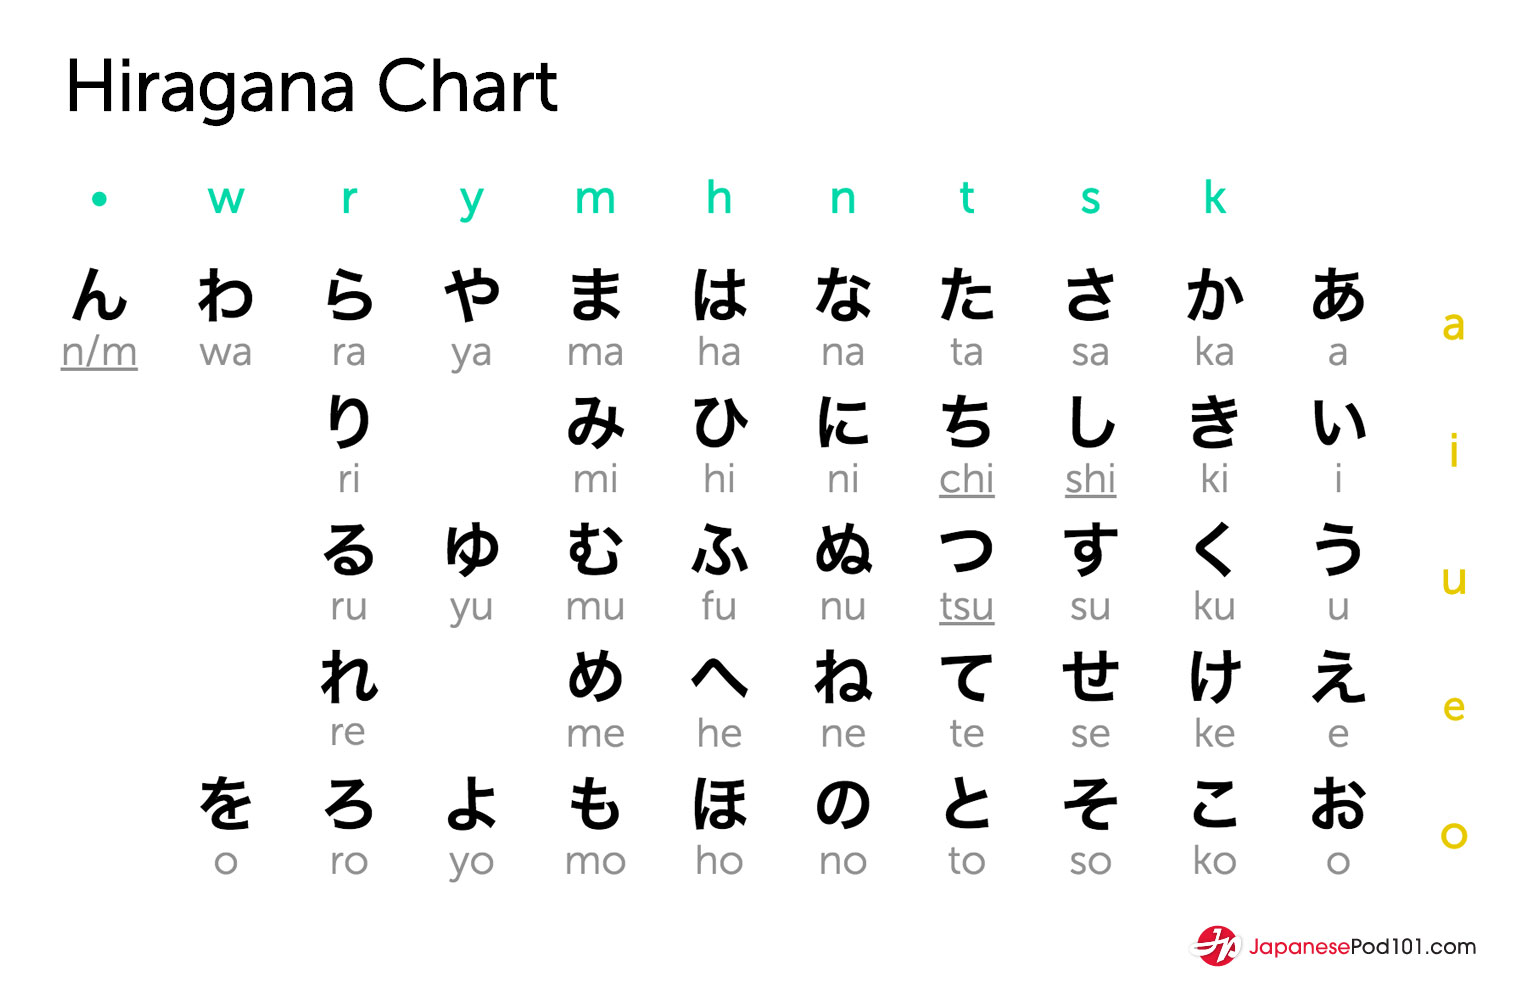
\includegraphics[scale=0.25]{res/hiragana_chart.jpg}
    \caption{Basic hiragana syllables}
\end{figure*}

\par
\textbf{Diacritic marks} - The basic syllables can be expanded upon by adding two short diagonal strokes ('') to convert the letters \{k$\to$g, s$\to$z, t$\to$d, h$\to$b\}. Also, the consonant \textit{h} changes to \textit{p} when you add a small circle.

\begin{figure*}[!ht]
    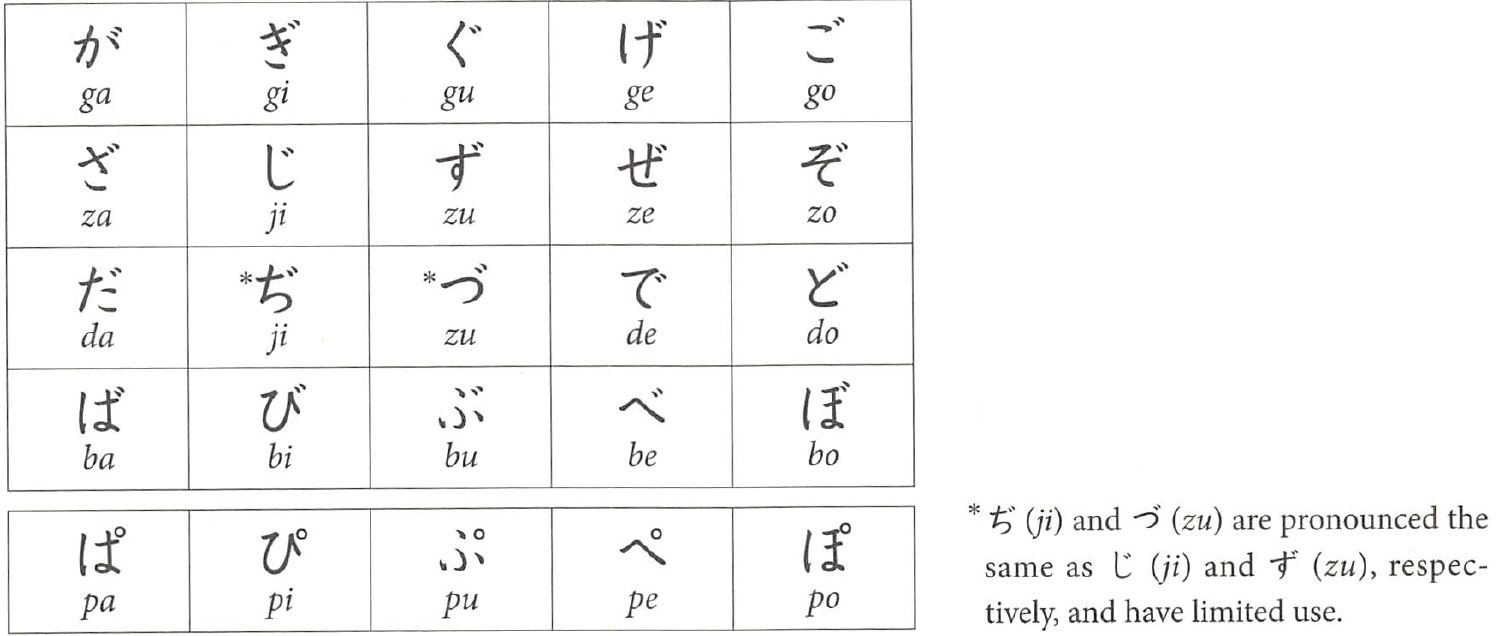
\includegraphics[scale=0.5]{res/hiragana_diacritics.jpg}
    \caption{Hiragana diacritics}
\end{figure*}

\par
\textbf{Diagraphs} - Contractions of sounds into one syllable can be represented by placing a \textit{small} character for either \textit{ya} (や), \textit{yu} (ゆ), or \textit{yo} (よ) after the original character for which you're trying to overwrite the sound. For example, \textit{chan} will be a combination of \textit{chi} and \textit{ya} to result in the \textit{cha} sound: ちゃん.

\begin{figure*}[!ht]
    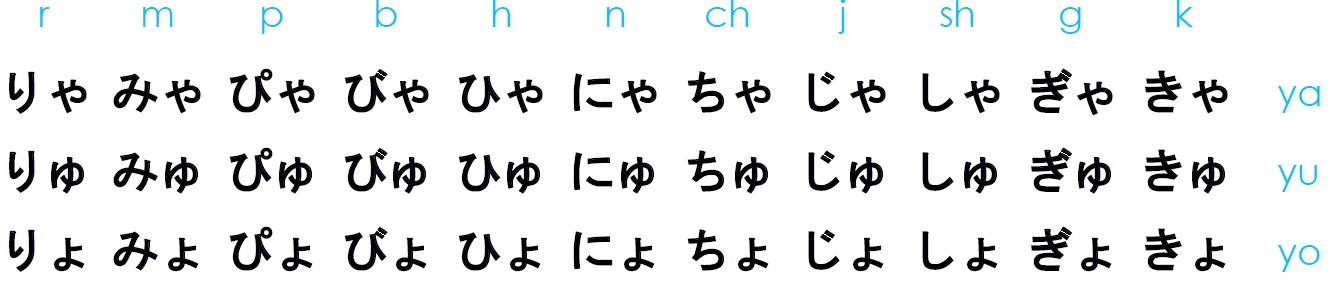
\includegraphics[scale=0.5]{res/hiragana_diagraphs.jpg}
    \caption{Hiragana contractions}
\end{figure*}


\textbf{\underline{Double Consonants}} \par
Finally, there is another small letter that looks like \textit{tsu} called the \textit{sokuon}, っ. This is used to show repeated consonants. I'm pretty sure that, because all hiragana end in a vowel sound, that this only applies to the first consonant of the following hiragana character. This means that, for example, かった, which is \textit{ka}-っ-\textit{ta}, would come out to \textit{ka\underline{t}ta} (won) as opposed to \textit{kata} (shoulder). Note that this isn't the case with double \textit{n}'s, which use ん. Some examples include:
\ul{
    \item か\underline{っ}た - \textit{ka\underline{t}ta} - won
    \item は\underline{っ}ぱ - \textit{ha\underline{p}pa} - leaf
    \item さ\underline{っ}か - \textit{sa\underline{k}ka} - writer
    \item さ\underline{ん}ねん - \textit{sa\underline{n}nen} - three years
}


\newpage
\subsection{Katakana}
Katakana is used for new words that didn't exist in Japan previously, including company names, scientific terms, and technology. Often, if you don't know the Japanese version of a word, you can say an English version of the word (e.g. \textit{ginkou} for bank could be understood with \textit{banku} instead). While hiragana is more curvy, katakana is more angular in nature.
\par
Katakana has diacritics and conjunctions, too. It also uses the sokuon letter, ッ, which is a small version of the letter for \textit{tsu}, ツ.
\par
Katakana also allows other small letter combinations (e.g. \q{halloween} $\to$ \furi{ハロ\underline{ウィ}ーン}{harowiin} where ウ is \textit{u} and イ is \textit{i}) in order to allow for sounds that aren't in the Japanese alphabet.
\par
Long vowels are written with the ー symbol. When writing vertically, the ー symbol is rotated 90 degrees, too.

\begin{figure*}
    \vspace{-3cm}  %the image was extra low for some reason, so this bumps it up a bit
    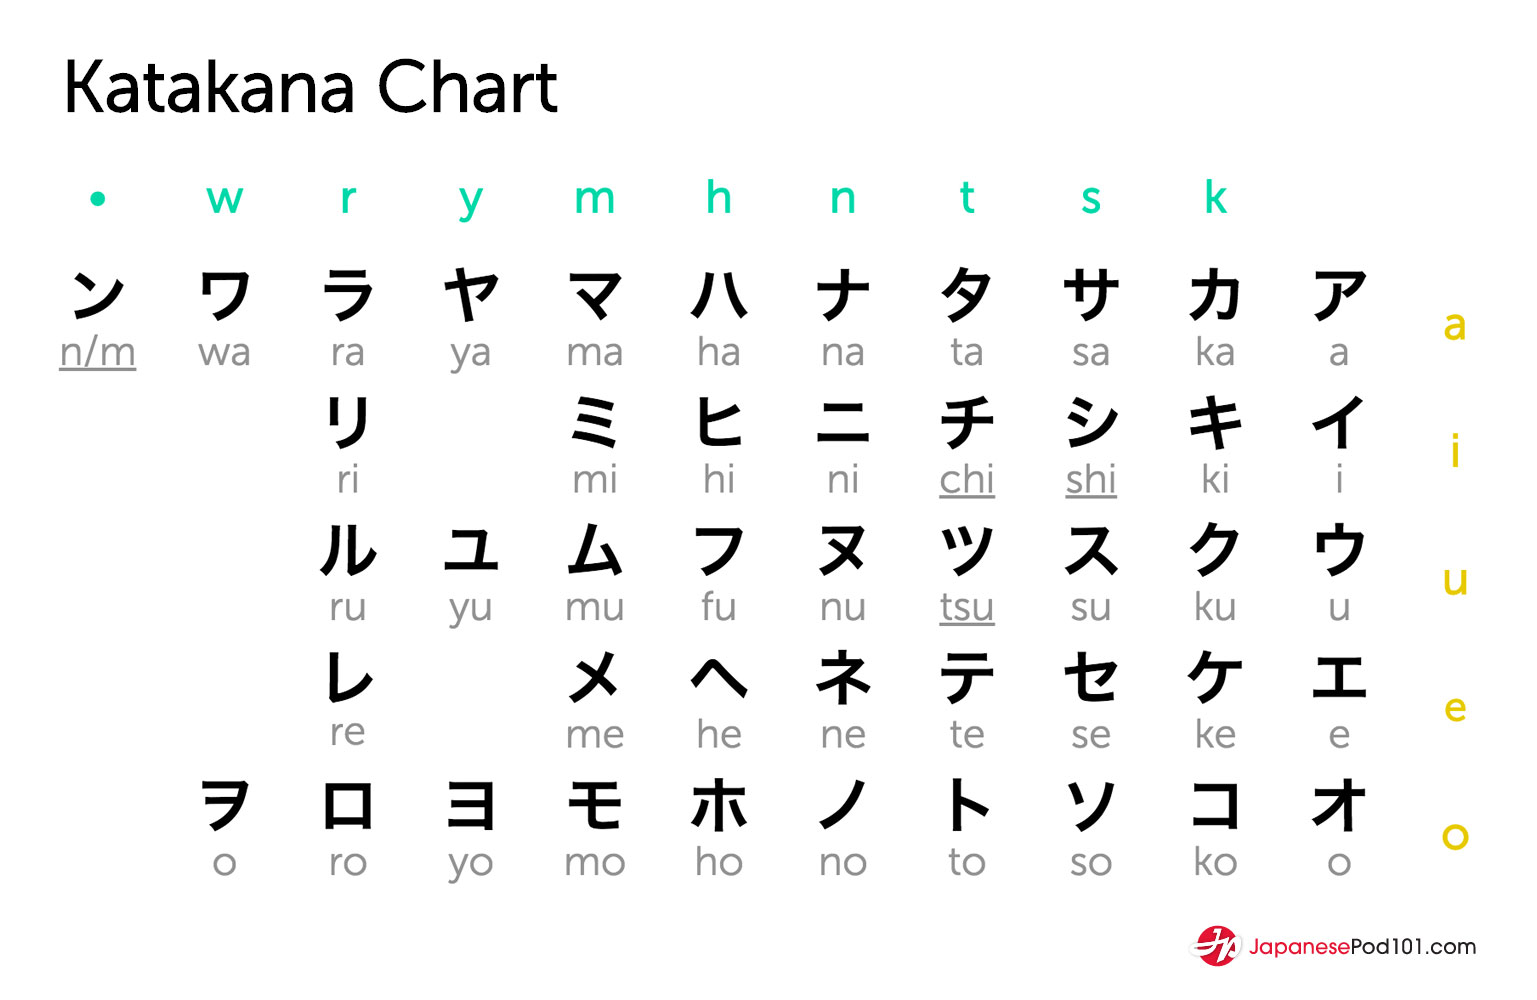
\includegraphics[scale=0.25]{res/katakana_chart.jpg}
    \caption{Basic katakana syllables}
\end{figure*}

\tab[|c|c|c|c|c|c|c|]{Practice}{
てテ & ちチ & こコ & らラ & をヲ & りリ & くク    \\\hline
なナ & ふフ & もモ & せセ & ひヒ & よヨ &     \\\hline
ぬヌ & るル & さサ & ゆユ & すス & みミ & ほホ    \\\hline
れレ & にニ & のノ & むム & とト & たタ & まマ    \\\hline
つツ & へヘ & わワ & めメ & しシ & ねネ & やヤ    \\\hline
はハ & きキ & そソ & けケ & かカ & じジ & ろロ    \\\hline
あア & いイ & うウ & えエ & おオ & んン &     \\\hline
}


\begin{figure*}[!ht]
    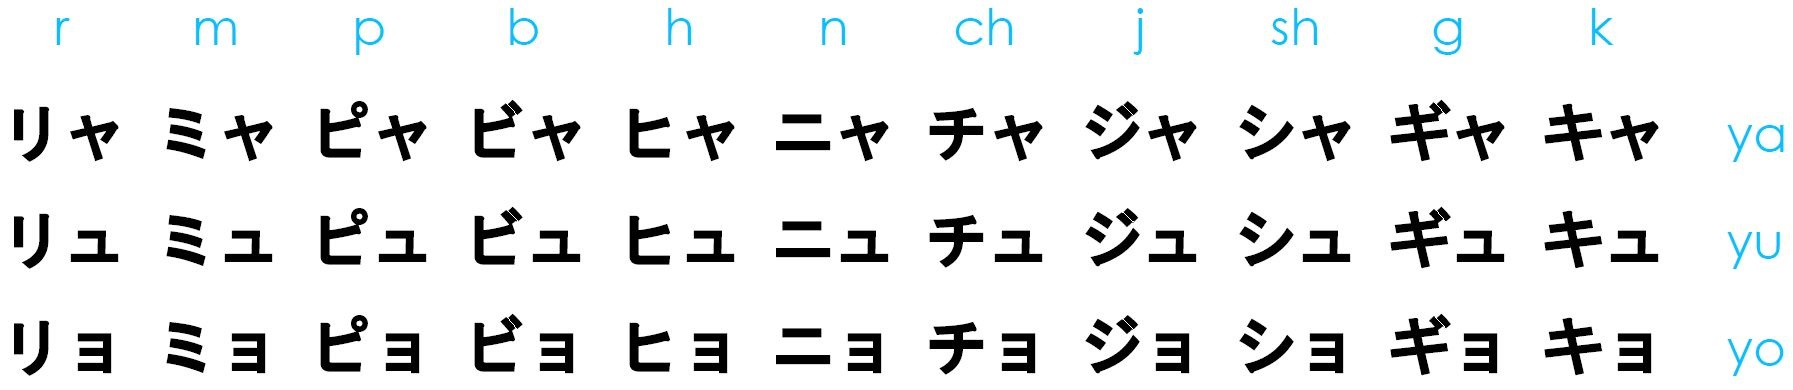
\includegraphics[scale=0.4]{res/katakana_diagraphs.jpg}
    \caption{Katakana contractions}
\end{figure*}

} %end document-wide \kana
\end{document}